% \iffalse      THIS IS A META-COMMENT
%<*dtx>
\ProvidesFile
%========================================================================
                       {NATBIB.DTX}
%========================================================================
%</dtx>
%% Copyright 1993-1999 Patrick W Daly
%% Max-Planck-Institut f\"ur Aeronomie
%% Max-Planck-Str. 2
%% D-37191 Katlenburg-Lindau
%% Germany
%% E-mail: daly@linmpi.mpg.de
% 
% This program can be redistributed and/or modified under the terms
% of the LaTeX Project Public License Distributed from CTAN
% archives in directory macros/latex/base/lppl.txt; either
% version 1 of the License, or any later version.
%
% This is a contributed file to the LaTeX2e system.
% -------------------------------------------------
% This is a LaTeX package to modify \cite and \thebibliography for author-year 
%    systems of bibliographic citation; will also work with 
%    numerical systems, allowing simplified style changes for them too.
% Installation:
%    LaTeX this file: creates docstrip installation file natbib.ins
%                         AND the (LaTeX2e) documentation
%    (La)TeX natbib.ins: creates package file natbib.sty 
%                        and optionally documentation driver natbib.drv
%    (natbib.ins may be edited as needed)
% Docstrip options available:
%        package - to produce a (LaTeX2e) package .sty file 
%        notes   - to produce a reference sheet for natbib usage
%        driver  - to produce a driver file to print the documentation
%        209     - (with package) for style file that runs under LaTeX 2.09 
%        subpack - (with package) for coding included in other packages
%        all     - (with package) to include all author-year systems
%                   else individually with:
%        apalike, newapa, chicago, harvard, authordate, astron
%        agu     - (with package,subpack) for inclusion in aguplus package
%        egs- (with package,subpack) for inclusion in egs package
%        nopreonly - allows \citestyle and \bibpunct to be used anywhere
%--------------------------------------------------------------------------
%<*!subpack>
%<package&209>\def\ProvidesPackage#1#2]
%<package&209>  {\typeout{Style option `#1'#2]}}
%
%  *** Identify the package file:-
%<package&!209>\NeedsTeXFormat{LaTeX2e}[1995/06/01]
% (Need LaTeX2e release 3 for option definition with single #)
%<package>\ProvidesPackage{natbib}
%</!subpack>
%
%  *** Provide command to dislay module version
%<package&subpack>\def\ModuleVersion#1[#2]{}
%<package&subpack>    \ModuleVersion{natbib}
%
%  *** Provide command to identify reference sheet (notes)
%<notes>\NeedsTeXFormat{LaTeX2e}
%<notes>\def\DescribesFile#1 [#2 #3 #4]
%<notes>  {\def\filename{#1}\def\filedate{#2}\def\fileversion{#3}}
%<notes>\DescribesFile{natbib}
%
%  *** Identify the driver file:-
%<driver>\NeedsTeXFormat{LaTeX2e}
%<driver>\ProvidesFile{natbib.drv}
%
%  *** The DATE, VERSION, and other INFO
%\fi
%\ProvidesFile{natbib}
        [1999/05/28 7.0 (PWD)]
% \changes{4.0}{1993 Aug 19}{First documented release}
% \changes{4.1}{1993 Oct 4}{Simplification of \cs{@citeapalk}}
% \changes{4.1a}{1993 Oct 14}{Add \texttt{rev} option for reversed comments 
%                             in \cs{cite}}
% \changes{4.1b}{1993 Oct 18}{Add \cs{bibfont} to list definition =\cs{relax}}
% \changes{4.2}{1993 Oct 22}{Add coding for AGU, NLINPROC}
% \changes{4.2}{1993 Nov 20}{Add more coding for AGU}
% \changes{4.3a}{1994 Feb 24}{First additions for \LaTeXe}
% \changes{5.0}{1994 May 18}{Revised for \LaTeXe{} and 2.09}
% \changes{5.0}{1994 May 18}{Remove obsolete JGR, GRL coding}
% \changes{5.0}{1994 May 18}{Add \cs{citeauthor}, \cs{citeyear}}
% \changes{5.0}{1994 May 18}{Two optional texts for \cs{cite} so \texttt{rev}
%                            option obsolete}
% \changes{5.0}{1994 May 18}{\LaTeXe\ options to select punctuation}
% \changes{5.1}{1994 Jun 22}{Conform to first official release of \LaTeXe}
% \changes{5.1}{1994 Jun 22}{Separate \LaTeX\ and 2.09 files}
% \changes{5.1}{1994 Jun 22}{Put doc driver first}
% \changes{5.2}{1994 Aug 25}{Fix up 2.09 style to run in compatibility mode}
% \changes{5.2}{1994 Aug 25}{\cs{citeauthor}, \cs{citeyear} make BibTeX 
%                             entry in aux file}
% \changes{5.2}{1994 Aug 25}{\cs{@citex} defined as in \LaTeXe}
% \changes{5.2}{1994 Aug 25}{Local config file \texttt{natbib.cfg} read in}
% \changes{5.3}{1994 Sep 13}{Add \cs{citefullauthor}, options \texttt{angle}, 
%                             \texttt{curly}}
% \changes{5.3}{1994 Sep 19}{Add star version of \cs{cite} for full authors}
% \changes{5.3}{1994 Sep 26}{Fix accents in citations with proper definition
%                             of \cs{protect}}
% \changes{5.4}{1994 Nov 24}{Add space in \cs{@citex} for text cites}
% \changes{5.4}{1994 Nov 24}{Replace \cs{if@tempswa} by \cs{ifNAT@swa}}
% \changes{5.4}{1994 Nov 24}{Add superscript citation type to \cs{bibpunct}}
% \changes{5.4}{1994 Nov 24}{Add \cs{@citesuper}, fix up bugs in superscripts}
% \changes{5.4}{1994 Nov 24}{Define \cs{@citexnum} as in \LaTeXe}
% \changes{5.4}{1995 Feb 03}{Add \cs{citestyle} same as \cs{bibstyle}}
% \changes{5.4}{1995 Feb 08}{For repeated years and authors, print just letter}
% \changes{5.5}{1995 Mar 13}{Add \cs{bibhang} and command space in
%      \cs{@cite}}
% \changes{5.5}{1995 Mar 16}{Add \cs{citealt} for citation with no
%      parentheses}
% \changes{5.5}{1995 Mar 24}{Reorganize internal commands, using \cs{NAT@}
%     prefixes}
% \changes{5.5}{1995 Mar 24}{Punctuation selection commands \cs{bibpunct},
%     \cs{citestyle} are now preamble only, whereas previously they had to
%     come after the preamble}
% \changes{5.5}{1995 May 14}{Change names of punctuation commands to
%     \cs{NAT@...}}
% \changes{6.0}{1995 Sep 4}{Allow numerical styles with author-year
%     \texttt{bst} files}
% \changes{6.0}{1995 Sep 21}{Add automatic indexing of citations}
% \changes{6.0}{1995 Sep 29}{Accommodate \texttt{index} package}
% \changes{6.1}{1995 Nov 22}{Fixed for \LaTeXe\ \texttt{1995/12/01}}
% \changes{6.1}{1995 Dec 4}{Make more robust against changes to internals}
% \changes{6.1a}{1995 Dec 19}{Fix test for changed citations}
% \changes{6.2}{1996 Jan 10}{Replace all \cs{uppercase}}
% \changes{6.2}{1996 Jan 11}{Add \cs{citet}}
% \changes{6.2}{1996 Feb 2}{Fix superscript size}
% \changes{6.2}{1996 Mar 05}{Add length \cs{bibsep} for linespacing between
%               references}
% \changes{6.2}{1996 Apr 15}{Fix clash with \texttt{amsart} and
%              \texttt{amsbook}}
% \changes{6.3}{1996 Jun 10}{Allow \texttt{showkeys} to be loaded first}
% \changes{6.3}{1996 Jun 17}{Fix punctuation for \texttt{plainnat}}
% \changes{6.3}{1996 Jun 17}{Suppress extra labels with numericals}
% \changes{6.4}{1996 Jun 18}{Provide \cs{bibname} and \cs{refname}}
% \changes{6.4}{1996 Jun 27}{Change \texttt{nlinproc} option to \texttt{egs}}
% \changes{6.4}{1996 Sep 1}{Make compatible with \texttt{chapterbib.sty}}
% \changes{6.4}{1996 Sep 12}{Fix spacing for superscripts}
% \changes{6.4}{1996 Sep 12}{Extra letter printed with \cs{citeyear}}
% \changes{6.4}{1996 Sep 13}{Add compression and sorting of numerical citations}
% \changes{6.4}{1996 Oct 2}{Make compatible with \texttt{hyperref.sty}}
% \changes{6.5}{1996 Dec 11}{KOMA script compatibility}
% \changes{6.5}{1997 Jan 10}{For EGS, no blank line between references}
% \changes{6.5}{1997 Jan 30}{Recode notes so they work with \cs{citet} and
%     \cs{citep}; change documentation to stress these commands over \cs{cite}}
% \changes{6.5}{1997 Feb 5}{Fix KOMA script properly}
% \changes{6.6}{1997 Apr 6}{Fix \cs{nocite} to work with \texttt{chapterbib}}
% \changes{6.6}{1997 May 26}{Let \cs{citealt} have full \cs{cite} syntax}
% \changes{6.6}{1997 Jun 4}{Add \cs{citeyearpar}}
% \changes{6.6}{1997 Jun 4}{Add sorting of author--year citations}
% \changes{6.6}{1997 Jun 12}{Add \cs{citealp} like \cs{citep} without parentheses}
% \changes{6.6}{1997 Jun 24}{Fix \texttt{showkeys} functionality}
% \changes{6.6}{1997 Jun 25}{Improve \texttt{hyperref} functionality}
% \changes{6.6}{1997 Jun 30}{Fix bug in \cs{NAT@citex}}
% \changes{6.7}{1997 Jul 14}{Add \texttt{longnamesfirst} option}
% \changes{6.7}{1997 Sep 12}{Fix interface with \texttt{showkeys}}
% \changes{6.7}{1997 Nov 10}{Fix interface with \texttt{babel}}
% \changes{6.7}{1997 Nov 11}{Add reference sheet extraction}
% \changes{6.8}{1997 Dec 1}{Permit \cs{@biblabel} to be user modified}
% \changes{6.8}{1998 Feb 19}{Fix hyperref bug in \cs{citep}}
% \changes{6.8a}{1998 Mar 6}{Correct wrong name for \texttt{longnamesfirst}
%    in the documentation}
% \changes{6.8a}{1998 May 14}{\cs{@biblabel} only redefinable for numerical
%    mode}
% \changes{6.8b}{1998 July 6}{Hyperref: to work with \texttt{chapterbib} and 
%     breaks links in textual citations}
% \changes{6.8c}{1998 July 14}{Hyperref: remove opening brace and notes from 
%     link}
% \changes{6.8d}{1998 Nov 23}{Fix bug in \texttt{super} option; suppress brackets}
% \changes{6.9}{1999 Jan 22}{Fix bug with \cs{makeindex}}
% \changes{6.9}{1999 Feb 23}{Update copyright notice}
% \changes{6.9}{1999 Mar 26}{Babel test made more general}
% \changes{7.0}{1999 May 7}{With empty year, act like \cs{citeauthor}}
% \changes{7.0}{1999 May 21}{Correct \cs{bibsection} for \texttt{amsbook}}
%
% \CheckSum{2346}
% \CharacterTable
%  {Upper-case    \A\B\C\D\E\F\G\H\I\J\K\L\M\N\O\P\Q\R\S\T\U\V\W\X\Y\Z
%   Lower-case    \a\b\c\d\e\f\g\h\i\j\k\l\m\n\o\p\q\r\s\t\u\v\w\x\y\z
%   Digits        \0\1\2\3\4\5\6\7\8\9
%   Exclamation   \!     Double quote  \"     Hash (number) \#
%   Dollar        \$     Percent       \%     Ampersand     \&
%   Acute accent  \'     Left paren    \(     Right paren   \)
%   Asterisk      \*     Plus          \+     Comma         \,
%   Minus         \-     Point         \.     Solidus       \/
%   Colon         \:     Semicolon     \;     Less than     \<
%   Equals        \=     Greater than  \>     Question mark \?
%   Commercial at \@     Left bracket  \[     Backslash     \\
%   Right bracket \]     Circumflex    \^     Underscore    \_
%   Grave accent  \`     Left brace    \{     Vertical bar  \|
%   Right brace   \}     Tilde         \~}
%
% \iffalse
%<*install>
%^^A =============================================
%^^A    Here is the docstrip installation file
%^^A    It is written on first LaTeX run if it 
%^^A    does not already exist
%^^A =============================================
\begin{filecontents*}{natbib.ins}
% File: natbib.ins
% Copyright 1999 Patrick W. Daly
%
% This file can be redistributed and/or modified under the terms
% of the LaTeX Project Public License Distributed from CTAN
% archives in directory macros/latex/base/lppl.txt; either
% version 1 of the License, or any later version.
% 
% It is an installation file for extracting package and driver
% files from the original source file. Simply process it under
% TeX or LaTeX. It works with Docstrip versions before and after
% December 1995.

\def\batchfile{natbib.ins}
\input docstrip

\preamble
=============================================
IMPORTANT NOTICE:

This program can be redistributed and/or modified under the terms
of the LaTeX Project Public License Distributed from CTAN
archives in directory macros/latex/base/lppl.txt; either
version 1 of the License, or any later version.

This is a generated file.
It may not be distributed without the original source file \inFileName.

Full documentation can be obtained by LaTeXing that original file.
Only a few abbreviated comments remain here to describe the usage.
=============================================
\endpreamble
\postamble

<<<<< End of generated file <<<<<<
\endpostamble
\keepsilent

% Docstrip before Dec 95 does not have \generate syntax, nor
%   \declarepreamble. Must redefine them. The \generateFile called
%   for each output file individually.
% Docstrip before Dec 96 cannot interprete multiline \if..\fi 
%   Thus for maximum compatibility, have only one-line conditionals

\let\oldDS F\relax
\expandafter\ifx\csname generate\endcsname\relax \let\oldDS T\relax\fi
\if\oldDS T  \def\declarepreamble#1{\preamble}\fi
\if\oldDS T  \def\declarepostamble#1{\postamble}\fi
\if\oldDS T  \generateFile{natbib.sty}{f}{\from{natbib.dtx}{package,all}} \fi

\declarepreamble\refsheet
=============================================
IMPORTANT NOTICE:

This program can be redistributed and/or modified under the terms
of the LaTeX Project Public License Distributed from CTAN
archives in directory macros/latex/base/lppl.txt; either
version 1 of the License, or any later version.

This is a generated file.
It may not be distributed without the original source file \inFileName.

This is a Reference Sheet for natbib. It consists of excerpts from the
original source file.

For more details, LaTeX the source \inFileName.
==============================================
\endpreamble

\declarepostamble\refsheetq

End of Reference Sheet file

\endpostamble

\ifx\oldDS T \generateFile{natnotes}{f}{\from{natbib.dtx}{notes}}\fi

\declarepreamble\driver
============================================
This is the driver file to produce the LaTeX documentation 
from the original source file \inFileName.

Make changes to it as needed. (Never change the file \inFileName!)
============================================
\endpreamble

\declarepostamble\driverq

End of documentation driver file.
\endpostamble

\ifx\oldDS T \generateFile{natbib.drv}{f}{\from{natbib.dtx}{driver}}\fi

\ifx\oldDS T \let\askforoverwritefalse\relax\def\generate#1{}\fi

\askforoverwritefalse
\generate{\file{natbib.sty}{\from{natbib.dtx}{package,all}}
          \file{natnotes}{\usepreamble\refsheet\usepostamble\refsheetq
                                \from{natbib.dtx}{notes}}
          \file{natbib.drv}{\usepreamble\driver\usepostamble\driverq
                           \from{natbib.dtx}{driver}}
         }

\obeyspaces
\Msg{*********************************************}%
\Msg{* For documentation, process natbib.dtx     *}%
\Msg{*    or the driver file      natbib.drv     *}%
\Msg{* For reference sheet, process natnotes.tex *}
\Msg{*********************************************}
\end{filecontents*}
%</install>
%<*driver>
\documentclass{ltxdoc}
%<driver>%\documentclass[twoside]{ltxdoc}
%<driver>%\documentclass[a4paper]{ltxdoc}
%<driver>%\documentclass[twoside,a4paper]{ltxdoc}
\raggedbottom

 %** To include the detailed explanation of the coding, comment out
 %**   the next line
\OnlyDescription

 %** To produce a command index: add the following line for one run,
 %**   then run  makeindex -s gind.ist natbib
 %**   and reprocess, with or without this line (much faster without)
%<driver>% \EnableCrossrefs\CodelineIndex 

 %** To produce a change history: add the following line for one run,
 %**   then run  makeindex -s gglo.ist -o natbib.gls natbib.glo
 %**   and reprocess, with or without this line (faster without)
%<driver>% \RecordChanges 

\DisableCrossrefs %May stay; zapped by \EnableCrossrefs
\CodelineNumbered %May stay

\begin{document}
   \DocInput{natbib.dtx}
\end{document}
%</driver>
%<*notes>
%^^A ***************************
%^^A Preamble to the Reference Sheet
%^^A ***************************
\documentclass{article}

\setlength{\parindent}{0pt}
\setlength{\parskip}{1ex}
\setlength{\textwidth}{\paperwidth}
\addtolength{\textwidth}{-2in}
\setlength{\oddsidemargin}{0pt}
\setlength{\textheight}{\paperheight}

\addtolength{\textheight}{-\headheight}
\addtolength{\textheight}{-\headsep}
\addtolength{\textheight}{-\footskip}
\addtolength{\textheight}{-2in}
\makeatletter
\def\@listI{\leftmargin\leftmargini
  \topsep\z@ \parsep\parskip \itemsep\z@}
\let\@listi\@listI
\@listi
\makeatother
\newcommand{\head}[1]{\subsubsection*{#1}}

\pagestyle{headings}
\markright{Reference sheet: \texttt{natbib}}

\usepackage{shortvrb}
\MakeShortVerb{\|}

\begin{document}
\thispagestyle{plain}

%</notes>
%\fi
%
% \DoNotIndex{\begin,\CodelineIndex,\CodelineNumbered,\def,\DisableCrossrefs}
% \DoNotIndex{\DocInput,\documentclass,\EnableCrossrefs,\end,\GetFileInfo}
% \DoNotIndex{\NeedsTeXFormat,\OnlyDescription,\RecordChanges,\usepackage}
% \DoNotIndex{\ProvidesClass,\ProvidesPackage,\ProvidesFile,\RequirePackage}
% \DoNotIndex{\LoadClass,\PassOptionsToClass,\PassOptionsToPackage}
% \DoNotIndex{\DeclareOption,\CurrentOption,\ProcessOptions,\ExecuteOptions}
% \DoNotIndex{\AtEndOfClass,\AtEndOfPackage,\AtBeginDocument,\AtEndDocument}
% \DoNotIndex{\InputIfFileExists,\IfFileExists,\ClassError,\PackageError}
% \DoNotIndex{\ClassWarning,\PackageWarning,\ClassWarningNoLine}
% \DoNotIndex{\PackageWarningNoLine,\ClassInfo,\PackageInfo,\MessageBreak}
% \DoNotIndex{\space,\protect,\DeclareRobustCommand,\CheckCommand}
% \DoNotIndex{\newcommand,\renewcommand,\providecommand,\newenvironment}
% \DoNotIndex{\renewenvironment,\newif,\newlength,\newcounter,\setlength}
% \DoNotIndex{\setcounter,\if,\ifx,\ifcase,\ifnum,\ifdim,\else,\fi}
% \DoNotIndex{\texttt,\textbf,\textrm,\textsl,\textsc,\reset@font}
% \DoNotIndex{\textup,\textit,\textmd,\textsf,\emph,\futurelet}
% \DoNotIndex{\ttfamily,\rmfamily,\sffamily,\mdseries,\bfseries,\upshape}
% \DoNotIndex{\slshape,\scshape,\itshape,\em,\LaTeX,\LaTeXe}
% \DoNotIndex{\filename,\fileversion,\filedate,\let,\makeindex}
% \DoNotIndex{\@auxout,\@for,\@gobble,\@ifnextchar,\@m,\@mkboth,\@nil}
% \DoNotIndex{\@noitemerr,\@tempa,\@tempswafalse,\@tempswatrue,\@warning}
% \DoNotIndex{\advance,\arabic,\AtBeginDocument,\bf,\bibname,\chapter}
% \DoNotIndex{\citation,\clubpenalty,\CodelineNumbered,\csname}
% \DoNotIndex{\DisableCrossrefs,\do,\edef,\else,\endcsname,\endlist}
% \DoNotIndex{\expandafter,\fi,\gdef,\global,\hbox,\hfill,\hskip,\hspace}
% \DoNotIndex{\if,\if@filesw,\if@tempswa,\ifx,\immediate,\itemindent,\labelsep}
% \DoNotIndex{\labelwidth,\lastskip,\leftmargin,\list,\mbox,\newblock}
% \DoNotIndex{\newpage,\p@enumiv,\parindent,\penalty,\refname}
% \DoNotIndex{\relax,\section,\settowidth,\sfcode,\sloppy,\small,\string}
% \DoNotIndex{\theenumiv,\thepage,\unskip,\uppercase,\usecounter,\vskip}
% \DoNotIndex{\widowpenalty,\write,\xdef,\z@,\catcode,\ifnum,\the}
% \DoNotIndex{\.,\@empty,\@ifundefined,\@latex@warning,\@minus,\@plus,\ }
% \DoNotIndex{\document,\@namedef,\@listi,\markboth,\or,\p@}
% \DoNotIndex{\listparindent,\noexpand,\par,\parsep,\pb,\pbf,\pbfseries}
% \DoNotIndex{\pc,\pd,\pem,\pit,\pitshape,\pmdseries,\prm,\prmfamily,\psc}
% \DoNotIndex{\pscshape,\psf,\psffamily,\psl,\pslshape,\ptt,\pttfamily}
% \DoNotIndex{\pupshape,\@iden,\@firstofone,\@unexpandable@protect}
% \DoNotIndex{\&,\{,\},\bibitem,\bibindent,\if@draft,\typeout}
% \DoNotIndex{\@ifclassloaded,\@ifstar,\@onlypreamble,\@preamblecmds}
% \DoNotIndex{\addtolength,\endinput,\@bsphack,\begingroup,\@wrindex}
% \DoNotIndex{\@listctr,\bibname,\enddocument,\hfil,\ignorespaces,\item}
% \DoNotIndex{\NAT@temp,\refname,\stepcounter,\@ifpackageloaded}
% \DoNotIndex{\@gobbletwo,\index,\itemsep,\markright,\scriptsize}
% \DoNotIndex{\textsuperscript,\@undefined}
% \DoNotIndex{\@celt,\@cite@list,\@citea,\@citeb,\@compress@cite}
% \DoNotIndex{\@bsphack,\@esphack,\@h@ld,\@make@cite@list,\@ne}
% \DoNotIndex{\@sort@celt,\@tempcnta,\@tempcntb,\delimiter,\endgroup}
% \DoNotIndex{\ifcat,\m@ne,\number}
% \DoNotIndex{\@markboth,\@mkboth,\nobreak,\SK@,\SK@@citex}
% \DoNotIndex{\SK@@label,\SK@@ref,SK@def,\SK@lbibitem,\bbl@redefine}
% \DoNotIndex{\@safe@activesfalse,\@save@activestrue,\active@prefix}
%
% \setcounter{IndexColumns}{2}
% \setlength{\IndexMin}{10cm}
% \setcounter{StandardModuleDepth}{1}
%
% \hyphenation{par-en-the-ti-cal}
%
% \GetFileInfo{natbib}
%
% \title{{\bfseries Natural Sciences Citations and References}\\
%         (Author--Year and Numerical Schemes)}
%    
% \author{Patrick W. Daly}
%         
% \date{This paper describes package \texttt{\filename}\\
%       version \fileversion{} from \filedate.
%  }
% 
% \maketitle
%
% \pagestyle{myheadings}
% \markboth{P. W. Daly}{NATURAL SCIENCES CITATIONS AND REFERENCES}
%
% \iffalse % The following lines belong to both the documentation and notes
%<*notes>
% \fi
\newcommand{\btx}{\textsc{Bib}\TeX}
\newcommand{\thestyle}{\texttt{\filename}}
% \iffalse % These lines belong only to the notes
\begin{center}{\bfseries\Large 
    Reference sheet for \thestyle\ usage}\\
    \large(Describing version \fileversion\ from \filedate)
\end{center}

\begin{quote}\slshape
For a more detailed description of the \thestyle\ package, \LaTeX\ the
source file \thestyle\texttt{.dtx}.
\end{quote}
%</notes>
% \fi
%
%^^A In order to keep all marginal notes on the one (left) side:
%^^A (otherwise they switch sides disasterously with twoside option)
% \makeatletter \@mparswitchfalse \makeatother 
%
% \begin{abstract}
% \iffalse % First line is Reference Sheet only, rest for both doc and Ref. Sheet
%<*notes>
\head{Overview}
% \fi
The \thestyle\ package is a reimplementation of the \LaTeX\ |\cite| command, 
to work with both author--year and numerical citations. It is compatible with 
the standard bibliographic style files, such as \texttt{plain.bst}, as well as 
with those for \texttt{harvard}, \texttt{apalike}, \texttt{chicago}, 
\texttt{astron}, \texttt{authordate}, and of course \thestyle. 

% \iffalse
%</notes>
% \fi
% In contrast to the packages listed above, the \thestyle{} package supports not 
% only the various author--year bibliography styles, but also those for standard 
% numerical citations. In fact, it can also produce numerical citations even 
% with an author--year bibliographic style, something that permits easy 
% switching between the two citation modes. To this end, replacements for the 
% standard \LaTeX\ \texttt{.bst} files are also provided. 
% 
% It is possible to define the citation \emph{style} (type of brackets and 
% punctuation between citations) and even to associate it with the name of 
% the bibliographic style so that it is automatically activated. Citation 
% styles can be defined for local \texttt{.bst} files by means of a 
% configuration file \thestyle\texttt{.cfg}. 
% 
% It is compatible with the packages: \texttt{babel}, \texttt{index}, 
% \texttt{showkeys}, \texttt{chapterbib}, \texttt{hyperref}, \texttt{koma} and 
% with the classes \texttt{amsbook} and \texttt{amsart}. It can also emulate the 
% sorting and compressing functions of the \texttt{cite} package (with which it 
% is otherwise incompatible). 
% 
% The \thestyle\ package therefore acts as a single, flexible interface for 
% most of the available bibliographic styles.
%
% \end{abstract}  
% 
% \newpage\tableofcontents\newpage
%
% \section{Introduction}
% The first problem of using author--year literature citations with standard
% \LaTeX{} is that the two forms of citations are not supported. These are:
% \begin{quote}
% textual: \dots\ as shown by Jones et al. (1990) \dots\\
% parenthetical: It has been shown (Jones et al., 1990) that \dots
% \end{quote}
% There is only one |\cite| command to do both jobs.
% 
% A second problem is that the \texttt{thebibliography} environment for
% listing the references insists on including the {\em labels\/} in the
% list. These labels are normally the numbers, needed for referencing. In
% the author--year system, they are superfluous and should be left off.
% Thus, if one were to make up a bibliography with the author--year as
% label, as
% \begin{quote}
% \begin{verbatim}
% \begin{thebibliography}{...}
% \bibitem[Jones et al., 1990]{jon90}
% Jones, P. K., . . .
% \end{thebibliography}
% \end{verbatim}
% \end{quote}
% then |\cite{jon90}| produces the parenthetical citation [Jones et al.,
% 1990], but there is no way to get the textual citation. Furthermore,
% the citation text will also be included in the list of references. 
% 
% The final problem is to find a \btx{} bibliography style that will be
% suitable.
% 
% \section{Previous Solutions}
% \begin{quote}\slshape
% This section may not be of interest to all users. To find out how to use
% \thestyle\ without reading about the historical background, go to
% Section~\ref{sec:usage}.
% \end{quote}
% 
% Although the author--year citation mode is not supported by
% \emph{standard} \LaTeX, there are a number of contributed packages that
% try to solve this problem. The various bibliographic styles
% (\texttt{.bst} files) that exist are usually tailored to be used with a
% particular \LaTeX{} package.
% 
% I have found a large number of \texttt{.bst} files on file servers that may
% act as indicators of the various systems available.
% 
% \subsection{The \texttt{natsci.bst} Style}
% What gave me my first inspiration was Stephen Gildea's \texttt{natsci.bst}
% for use with his \texttt{agujgr.sty} file. This showed me that the problem
% was solvable. However, Gildea's style formats |\bibitem| just as I
% illustrated above: with an optional label consisting of abbreviated
% authors and year. Thus only parenthetical citations can be accommodated.
% The list of references, however, is fixed up in his style files.
% 
% \subsection{The \texttt{apalike.bst} Style}
% Oren Patashnik, the originator of \btx{} and the standard \texttt{.bst}
% files, has also worked on an author--year style, called \texttt{apalike.bst}
% with a corresponding \texttt{apalike.sty} to support it. Again, only the
% parenthetical citation is provided. Except for the fact that his style
% works with version~0.99 of \btx, its functionality is identical to that
% of the \texttt{natsci} files.
% 
% Patashnik does not like author--year citations. He makes this very clear
% in his \btx{} manuals and in the header to \texttt{apalike.bst}.
% Nevertheless, one should respect his work in this area, simply because he
% should be the best expert on matters of \btx. Thus \texttt{apalike.bst}
% could be the basis for other styles.
% 
% The form of the \texttt{thebibliography} entries in this system is
% \begin{quote}
% |\bibitem[Jones et al., 1990]{jon90}...|
% \end{quote}
% the same as I illustrated earlier. This is the most minimal form that can
% be given. I name it the \texttt{apalike} variant, after Patashnik's 
% \texttt{apalike.bst} and \texttt{apalike.sty}. However, there could be many
% independent \texttt{.bst} files that follow this line.
% 
% The bibliography style files belonging to this group include:
% \begin{quote}
% \texttt{apalike}, \texttt{apalike2}, \texttt{cea}, \texttt{cell}, 
% \texttt{jmb}, \texttt{phapalik}, \texttt{phppcf}, \texttt{phrmp}
% \end{quote}
% 
% \subsection{The \texttt{newapa} Style}
% A major improvement has been achieved with \texttt{newapa.bst} and the
% accompanying \texttt{newapa.sty} files by Stephen N. Spencer and Young U.
% Ryu. Under their system, three separate items of information are included
% in the |\bibitem| label, to be used as required. These are: the full
% author list, the abbreviated list, and the year. This is accomplished by
% means of a |\citeauthoryear| command included in the label, as
% \begin{quote}
% |\bibitem[\protect\citeauthoryear{Jones, Barker,|\\
% |  and Williams}{Jones et al.}{1990}]{jon90}...|
% \end{quote}
% Actually, this only illustrates the basic structure of |\citeauthoryear|;
% the \texttt{newapa} files go even further to replace some words and 
% punctuation
% with commands. For example, the word `and' above is really
% |\betweenauthors|, something that must be defined in the \texttt{.sty} file.
% Of course, |\citeauthoryear| is also defined in that file. A
% number of different |\cite| commands are available to print out the
% citation with complete author list, with the short list, with or without
% the date, the textual or parenthetical form. 
% 
% Thus the |\citeauthoryear| entry in |\bibitem| is very flexible,
% permitting the style file to generate every citation form that one might
% want. It is used by a number of other styles, with corresponding
% \texttt{.sty} files. They all appear to have been inspired by 
% \texttt{newapa.bst}, although they lack the extra punctuation commands. 
% 
% Bibliographic style files belonging to the \texttt{newapa} group include
% \begin{quote}
% \texttt{newapa}, \texttt{chicago}, \texttt{chicagoa}, \texttt{jas99}, 
% \texttt{named}
% \end{quote}
% Note: the last of these, \texttt{named.bst}, uses |\citeauthoryear| in a
% slightly different manner, with only two arguments: the short list and
% year.
% 
% \subsection{The Harvard Family}
% The same effect is achieved by a different approach in the Harvard family
% of bibliographic styles. Here a substitute for |\bibitem| is used, as
% \begin{quote}
% |\harvarditem[Jones et al.]{Jones, Baker, and|\\
% |   Williams}{1990}{jon90}...|
% \end{quote}
% The accompanying interface package file is called \texttt{harvard.sty}
% and is written by Peter Williams and Thorsten Schnier. It
% defines |\harvarditem| as well as the citation commands |\cite|, for
% parenthentical, and |\citeasnoun|, for textual citations. The first
% citation uses the long author list, following ones the shorter list, if
% it has been given in the optional argument to |\harvarditem|.
% 
% Bibliography styles belonging to the Harvard family are
% \begin{quote}
% \texttt{agsm}, \texttt{dcu}, \texttt{kluwer}
% \end{quote}
% 
% This package has been updated for \LaTeXe, with many additions to
% add flexibility. The result is a powerful interface that should meet most
% citation needs. (It does not suppress repeated authors, though,
% as \thestyle{} does.)
%
% \subsection{The Astronomy Style}
% Apparently realizing the limitations of his \texttt{apalike} system, Oren
% Patashnik went on to develop a `true' \texttt{apa} bibliographic style,
% making use of the method already employed by an astronomy journal. This
% is actually very similar to the \texttt{newapa} label but with only the
% short list of authors:
% \begin{quote}
% |\bibitem[\protect\astroncite{Jones et al.}{1990}]{jon90}|\\
% |   ...|
% \end{quote}
% It requires the package file \texttt{astron.sty} 
% or any other style that defines |\astroncite| appropriately.
% 
% Bibliographic styles belonging to the astronomy group are
% \begin{quote}
% \texttt{apa}, \texttt{astron}, \texttt{bbs}, \texttt{cbe}, 
% \texttt{humanbio}, \texttt{humannat}, \texttt{jtb}
% \end{quote}
% 
% This is as good as the |\citeauthoryear| command, although not as
% flexible since the full list of authors is missing.
% 
% \subsection{The \texttt{authordate} Style}
% Finally, I have also found some packages making use of a label command
% called |\citename| in the form
% \begin{quote}
% |\bibitem[\protect\citename{Jones et al., }1990]{jon90}|\\
% |    ...|
% \end{quote}
% 
% This is not a good system since the author list and date are not cleanly
% separated as individual arguments, and since the punctuation is included
% in the label text. It is better to keep the punctuation fully removed, as
% part of the definitions in the \texttt{.sty} file, for complete flexibility.
% 
% Bibliographic styles belonging to this group are
% \begin{quote}
% \texttt{authordate1}, \texttt{authordate2}, \texttt{authordate3}, 
% \texttt{authordate4}, \texttt{aaai-named}
% \end{quote}
% with accompanying style file \texttt{authordate1-4.sty}.
% 
% \section{The \thestyle{} System}
% The form of the |\bibitem| entry that I have used for all my
% bibliographic styles is only slightly more complicated than the minimal
% one, but allows a clean separation between authors and date:
% \begin{quote}
% |\bibitem[Jones et al.(1990)]{jon90}...|\\[1ex]
% or alternatively\\[1ex]
% |\bibitem[Jones et al.(1990)Jones, Baker, |\\
% \hspace*{2em}|and Williams]{jon90}...|
% \end{quote}
%
% (One weakness of the \thestyle{} format is that it fails if the author
% list itself contains parentheses! This may be fixed up if the author list
% is grouped in curly braces.)
% 
% I wanted to name the system something like `natural sciences bibliography',
% intending it to be a variant of \texttt{natsci.sty}. Since that name
% was already taken, I resorted to the rather cryptic, and definitely ugly,
% \thestyle.
% 
% The \thestyle\texttt{.sty} package\footnote{Formerly called a \emph{style 
% file} in the older \LaTeX~2.09 terminology.} supports not only my own 
% |\bibitem| format, but also all the others described here, plus numerical 
% citation modes. The additional questions of citation style (type of brackets, 
% commas or semi-colons between citations) can be defined once and for all for 
% each \texttt{.bst} file and need never be specified explicitly in the source 
% text. The |\cite| commands and syntax are always those of \thestyle, even 
% when used with a \texttt{.bst} file such as \texttt{chicago.bst} that would 
% normally have a different set of commands (defined in \texttt{chicago.sty}).
% The result is a single \LaTeX{} package to handle {\em all\/} the 
% bibliographic styles in a uniform manner. 
% 
% All the author--year bibliographic style files can also be used for
% \emph{numerical} citations, by simply selecting the mode in one of the
% ways described in Sections~\ref{sec:bibpunct} and \ref{sec:opts}. It is
% not possible to employ author-year citations with pure numerical
% \texttt{.bst} files, and never will be.  
% See Section~\ref{sec:6.0} for more information.
% 
% \section{Using this Package}\label{sec:usage}
% 
% \iffalse
%<*notes>
\head{Loading}
Load with |\usepackage[|\emph{options}|]{|\thestyle|}|. See list of
\emph{options} at the end.

%</notes>
% \fi
% In this paper, I distinguish between the citation \emph{mode} (author--year
% or numerical) and citation \emph{style} (the type of punctuation used for
% citations). The citation style is something that is independent of the
% bibliography style and is not programmed in the \texttt{.bst} files.
% 
% \subsection{New Bibliography Styles}\label{sec:plainnat}
% 
% \iffalse
%<*notes>
\head{Replacement bibliography styles}
% \fi
I provide three new \texttt{.bst} files to replace the standard \LaTeX\
numerical ones:
\begin{quote}\ttfamily
 plainnat.bst \qquad abbrvnat.bst \qquad unsrtnat.bst
\end{quote}
% \iffalse
%</notes>
% \fi
% These produce reference lists in the same style as the corresponding
% standard \texttt{.bst} file, but work with \thestyle{}. The
% advantage is that they can be used in both numerical and author--year
% mode.
% 
% These \texttt{.bst} files are not meant to be exhaustive by any means. Other 
% style files conforming to the \thestyle{} format exist, or may be generated 
% with my \texttt{custom-bib} (also known as \texttt{makebst}) program.
% 
% \subsection{Basic Citation Commands}
% 
% \DescribeMacro{\citet}
% \DescribeMacro{\citep}
% \iffalse
%<*notes>
\head{Basic commands}
% \fi
The \thestyle\ package has two basic citation commands, |\citet| and
|\citep| for \emph{textual} and \emph{parenthetical} citations, respectively.
There also exist the starred versions |\citet*| and |\citep*| that print
the full author list, and not just the abbreviated one.
All of these may take one or two optional arguments to add some text before
and after the citation.
\begin{quote}
\begin{tabular}{l@{\quad$\Rightarrow$\quad}l}
  |\citet{jon90}| & Jones et al. (1990)\\
  |\citet[chap.~2]{jon90}| & Jones et al. (1990, chap.~2)\\[0.5ex]
  |\citep{jon90}| & (Jones et al., 1990)\\
  |\citep[chap.~2]{jon90}| & (Jones et al., 1990, chap.~2)\\
  |\citep[see][]{jon90}| & (see Jones et al., 1990)\\
  |\citep[see][chap.~2]{jon90}| & (see Jones et al., 1990, chap.~2)\\[0.5ex]
  |\citet*{jon90}| & Jones, Baker, and Williams (1990)\\
  |\citep*{jon90}| & (Jones, Baker, and Williams, 1990)
\end{tabular}
\end{quote}
% \iffalse
%</notes>
% \fi
% The starred versions can only list the full authors if the \texttt{.bst}
% file supports this feature; otherwise, the abbreviated list is printed.
%
% In standard \LaTeX, the |\cite| command can only take a single optional
% text for a note after the citation; here, a single optional text is a
% post-note, while two are the pre- and post-notes. To have only a pre-note, it
% is necessary to provide an empty post-note text, as shown above.
%
% More complex mixtures of text and citations can be generated with the
% all-purpose |\citetext| command in Section~\ref{sec:excite}.
% 
% \iffalse
%<*notes>
\head{Multiple citations}
% \fi
Multiple citations may be made by including more than one
citation key in the |\cite| command argument. 
% \textsl{If adjacent citations
% have the same author designation but different years, then the author
% names are not reprinted.}
\begin{quote}
\begin{tabular}{l@{\quad$\Rightarrow$\quad}l}
  |\citet{jon90,jam91}| & Jones et al. (1990); James et al. (1991)\\
  |\citep{jon90,jam91}| & (Jones et al., 1990; James et al. 1991)\\
  |\citep{jon90,jon91}| & (Jones et al., 1990, 1991)\\
  |\citep{jon90a,jon90b}| & (Jones et al., 1990a,b)
\end{tabular}
\end{quote}

% \iffalse
\head{Numerical mode}
% \fi
These examples are for author--year citation mode. In numerical mode, the 
results are different.
\begin{quote}
\begin{tabular}{l@{\quad$\Rightarrow$\quad}l}
  |\citet{jon90}| & Jones et al. [21]\\
  |\citet[chap.~2]{jon90}| & Jones et al. [21, chap.~2]\\[0.5ex]
  |\citep{jon90}| & [21]\\
  |\citep[chap.~2]{jon90}| & [21, chap.~2]\\
  |\citep[see][]{jon90}| & [see 21]\\
  |\citep[see][chap.~2]{jon90}| & [see 21, chap.~2]\\[0.5ex]
  |\citep{jon90a,jon90b}| & [21, 32]
\end{tabular}
\end{quote}
% \iffalse
%</notes>
% \fi
% The authors can only be listed if the \texttt{.bst} file supports
% author--year citations. The standard \texttt{.bst} files, such as
% \texttt{plain.bst} are numerical only and transfer no author--year
% information to \LaTeX. In this case, |\citet| prints ``\textbf{(author?)} 
% [21].''
% 
% \DescribeMacro{\cite}
% In the original versions of \thestyle, the traditional |\cite| command was
% used for both textual and parenthetical citations. The presence of an empty
% optional text in square brackets signalled parenthetical. This syntax has been
% retained for compatibility, but is no longer encouraged.
% 
% This means that |\cite| (without notes) is the same as |\citet| in
% author--year mode, whereas in numerical mode, it is the same as |\citep|.
% The starred version, as well as the one or two optional notes, may also be
% used.
%
% It is possible to have multiple citations sorted into the same sequence as 
% they appear in the list of references, regardless of their order as 
% arguments to the |\cite| commands. The option \texttt{sort} is required for 
% this feature. See Section~\ref{sec:sort}.
% 
% Some publishers require that the first citation of any given reference be 
% given with the full author list, but that all subsequent ones with the 
% abbreviated list. Include the option \texttt{longnamesfirst} to enable this for 
% \thestyle. See Section~\ref{sec:long}.
% 
% \subsection{Extended Citation Commands}
% \label{sec:excite}
% 
% \DescribeMacro{\citealt}
% \DescribeMacro{\citealp}
% \DescribeMacro{\citetext}
% \iffalse
%<*notes>
\head{Suppressed parentheses}
% \fi
As an alternative form of citation, |\citealt| is the same as |\citet| but 
\emph{without parentheses}. Similarly, |\citealp| is |\citep| without  
parentheses. Multiple references, notes, and the starred variants 
also exist. 
\begin{quote}
\begin{tabular}{l@{\quad$\Rightarrow$\quad}l}
  |\citealt{jon90}| & Jones et al.\ 1990\\
  |\citealt*{jon90}| & Jones, Baker, and Williams 1990\\
  |\citealp{jon90}| & Jones et al., 1990\\
  |\citealp*{jon90}| & Jones, Baker, and Williams, 1990\\
  |\citealp{jon90,jam91}| & Jones et al., 1990; James et al., 1991\\
  |\citealp[pg.~32]{jon90}| & Jones et al., 1990, pg.~32\\
  |\citetext{priv.\ comm.}| & (priv.\ comm.)
\end{tabular}
\end{quote}
The |\citetext| command 
allows arbitrary text to be placed in the current citation parentheses. 
This may be used in combination with |\citealp|.
% For example, 
% \begin{verbatim}
% \citetext{see \citealp{jon90}, 
%   or even better \citealp{jam91}}
% \end{verbatim}
% to produce (see Jones et al., 1990, or even better James et al., 1991).
%
% \iffalse
%</notes>
% \fi
%
% \DescribeMacro{\citeauthor}
% \DescribeMacro{\citeyear}
% \DescribeMacro{\citeyearpar}
% \DescribeMacro{\citefullauthor}
% \iffalse
%<*notes>
\head{Partial citations}
% \fi
In author--year schemes, it is sometimes desirable to be able to refer to
the authors without the year, or vice versa. This is provided with the
extra commands
\begin{quote}
\begin{tabular}{l@{\quad$\Rightarrow$\quad}l}
  |\citeauthor{jon90}| & Jones et al.\\
  |\citeauthor*{jon90}| & Jones, Baker, and Williams\\
  |\citeyear{jon90}|   & 1990\\
  |\citeyearpar{jon90}| & (1990)
\end{tabular}
\end{quote}
% \iffalse
%</notes>
% \fi
% There also exists a command |\citefullauthor| which is equivalent to 
% |\citeauthor*|.
% 
% If the full author information is missing, then |\citeauthor*| is
% the same as |\citeauthor|, printing only the abbreviated list.
% This also applies to the starred versions of |\citet| and |\citep|.
% 
% If the author or year information is missing (as is the case with the
% standard \LaTeX{} \texttt{.bst} files), these commands issue a warning.
% 
% \medskip\noindent
% \textbf{Note:}
% these commands may also be used with numerical
% citations, provided an author--year \texttt{.bst} file is being employed.
% 
% \medskip\noindent
% \textbf{Note:} all |\cite..| commands have the same 
% syntax, allowing multiple citations and up to two notes (there is, however, 
% no starred |\citeyear| variant). It does not really make much sense to add 
% notes to |\citeyear| and |\citeauthor|, especially with multiple citations; 
% however, this can be done, there will be no error message, but the results 
% are sometimes strange. For example, in numerical mode, the notes are fully 
% ignored, while in author--year mode, only the post-note is accepted. 
% Multiple citations in |\citet| are also not recommended (nor are they in my 
% opinion meaningful), but if they are used with notes, the pre-note will 
% appear before each year, and the post-note only after the last year. These 
% are admittedly bugs, but the effort to remove them is not justified by the 
% questionable usefulness of these features. 
%
% In summary, notes are only intended for |\citep| but they may also be used 
% with |\citet| in author--year mode, with single citations. In any other 
% situation, the results are unpredictable. 
% 
% \DescribeMacro{\Citet}
% \DescribeMacro{\Citep}
% \DescribeMacro{\Citealt}
% \DescribeMacro{\Citealp}
% \DescribeMacro{\Citeauthor}
% \subsection{Forcing Upper Cased Name}
% \iffalse
%<*notes>
\head{Forcing upper cased names}
% \fi
If the first author's name contains a \textsl{von} part, such as ``della 
Robbia'', then |\citet{dRob98}| produces ``della Robbia (1998)'', even at the 
beginning of a sentence. One can force the first letter to be in upper case 
with the command |\Citet| instead. Other upper case commands also exist.
\begin{quote}
\begin{tabular}{rl@{\quad$\Rightarrow$\quad}l}
  when & |\citet{dRob98}| & della Robbia (1998) \\
  then & |\Citet{dRob98}| & Della Robbia (1998) \\
     &   |\Citep{dRob98}| & (Della Robbia, 1998) \\
     &   |\Citealt{dRob98}| & Della Robbia 1998 \\
     &   |\Citealp{dRob98}| & Della Robbia, 1998 \\
     &   |\Citeauthor{dRob98}| & Della Robbia 
\end{tabular}
\end{quote}
These commands also exist in starred versions for full author names.

% \textbf{Note:} the coding for the upper casing commands is tricky and likely 
% buggy. It operates on the names that are stored in the |\bibitem| entry, and 
% works even if old style font commands are used; however, NFSS commands will 
% cause it to crash. Thus
% \begin{tabular}{ll}
%   |\bibitem[{\it della Robbia}(1998)]{dRob98}| & is okay, but \\
%   |\bibitem[\textit{della Robbia}(1998)]{dRob98}| & crashes.
% \end{tabular}
% I hope to improve this situation in future.
% 
% \iffalse
%</notes>
% \fi
%
% \subsection{Citation Aliasing}
% \DescribeMacro{\defcitealias}
% \DescribeMacro{\citetalias}
% \DescribeMacro{\citepalias}
% \iffalse
%<*notes>
\head{Citation aliasing}
% \fi
Sometimes one wants to refer to a reference with a special designation, 
rather than by the authors, i.e. as Paper~I, Paper~II. Such aliases can be 
defined and used, textual and/or parenthetical with:
\begin{quote}
\begin{tabular}{lcl}
  |\defcitealias{jon90}{Paper~I}|\\
  |\citetalias{jon90}| & $\Rightarrow$ & Paper~I\\
  |\citepalias{jon90}| & $\Rightarrow$ & (Paper~I)
\end{tabular}
\end{quote}
These citation commands function much like |\citet| and |\citep|: they may 
take multiple keys in the argument, may contain notes, and are marked as
hyperlinks.
% \iffalse
%</notes>
% \fi
% 
% A warning is issued if the alias is used before it is defined, or if an alias 
% is redefined for a given citation. No warning is issued if an alias is 
% defined for a citation key that does not exist; the warning comes when it is 
% used!
% 
% See Section~\ref{sec:yearless} for an alternative means of citing with
% a code name.
%
% \subsection{Authorless and Yearless References}\label{sec:yearless}
% What does one do about references that do not have authors? This has long 
% bothered me but I do have a suggestion. Standard \btx\ styles make use of a 
% \texttt{KEY} field in the entries to be used for alphabetizing when the 
% authors or editors are missing. The author--year styles go even further and 
% insert the \texttt{KEY} field in place of the authors. One can imagine giving 
% a code designation for the work at this point. For example,
% \begin{quote}
% \begin{verbatim}
% @MANUAL{handbk98,
%   title = {Assembling Computers},
%   year = 1998,
%   organization = {MacroHard Inc.},
%   key = "MH-MAN"
% }
% \end{verbatim}
% \end{quote}
% With \texttt{plain}, the key text \texttt{MH-MAN} is used only to order the 
% reference, but with \texttt{plainnat} and other author--year styles, it is 
% used in place of the authors. One can then refer to it as 
% |\citeauthor{handbk98}| to get MH-MAN or as |\citetext{\citeauthor{handbk98}}| 
% for (MH-MAN), a parenthetical citation.
% 
% This can be greatly simplified if
% the bibliography style leaves the date blank in the |\bibitem| 
% entry, as 
% \begin{quote}
% |\bibitem[MH-MAN()]{handbk98}|
% \end{quote}
% for then \thestyle\ suppresses the date, preceding punctuation, and the 
% braces for |\citet|. This means that |\citet| and |\citep| behave 
% automatically like the two examples above. 
% The date still may appear in the text of the reference.
% 
% The \thestyle\ bibliography styles have been modified accordingly to omit
% the date from the |\bibitem| entry when missing authors and/or editors 
% are replaced by key text.
% 
% Similarly, if the year is missing, it will be left blank in the |\bibitem| 
% entry; thus citing such a work will only produce the authors' names.
% 
% \textbf{Note:} there are many other possibilities with this feature. One can 
% even produce citations like those of the \texttt{alpha} bibliography style, 
% by placing the citation code in place of the authors in the |\bibitem| entry 
% and leaving the year blank. A second code (or maybe even the authors 
% themselves) could be placed where the full author list normally appears, to 
% be printed with the starred version of the |\cite| commands. For example,
% \begin{quote}
% |\bibitem[MH-MAN()MacroHard Inc.]{handbk98}|
% \end{quote}
% 
% \subsection{Extra Features in the \texttt{plainnat} Family}\label{sec:url}
%
% The special \texttt{.bst} files for \thestyle\ mentioned in 
% Section~\ref{sec:plainnat} have a number of extra fields compared to the 
% original files: \\
% \begin{tabular}{ll}
% \texttt{ISBN} & for the ISBN number in books,\\
% \texttt{ISSN} & for the ISSN number in periodicals,\\
% \texttt{URL} & for the Internet address of on-line documents.
% \end{tabular}
% The URL address is set in a typewriter font and often leads to line-breaking 
% problems. It is advisable to load the \texttt{url} package of Donald 
% Arseneau, which allows typewriter text to be broken at punctuation marks. The 
% URL addresses are set with the |\url| command in this package, but if it is 
% not loaded, then |\url| is defined to be |\texttt|, with no line breaks. 
% 
% As pointed out in Section~\ref{sec:yearless}, the \texttt{KEY} field is 
% treated differently by \texttt{plainnat} than in \texttt{plain}. Whereas the 
% latter uses this field only to alphabetize entries without authors, 
% \texttt{plainnat} actually inserts it in place of the author, both in the 
% reference text and in the citation label (|\bibitem| entries). Furthermore, 
% the year is left empty in |\bibitem| so that |\citep| prints only the 
% ``author'' text, which is now the \texttt{KEY}. This should be some code 
% designation for the work.
% 
% \subsection{Selecting Citation Punctuation}\label{sec:bibpunct}
%
% \DescribeMacro{\bibpunct}
% The above examples have been printed with the default citation style.
% It is possible to change this, as well as to select numerical or
% author--year mode, by means of the |\bibpunct| command, which takes 
% one optional and 6 mandatory arguments. The mandatory ones are:
% \iffalse
%<*notes>
\head{Selecting citation style and punctuation}
Use the command |\bibpunct| with one optional and 6 mandatory arguments:
% \fi
\begin{enumerate}
\item the opening bracket symbol, default = (
\item the closing bracket symbol, default = )
\item the punctuation between multiple citations, default = ;
\item the letter `n' for numerical style, or `s' for numerical superscript
      style, any other letter for
      author--year, default = author--year; 
%       note, it is not necessary to
%       specify which author--year interface is being used, for all will be
%       recognized;
\item the punctuation that comes between the author names and the year
%       (parenthetical case only), default = ,
\item the punctuation that comes between years or numbers when common author 
      lists are suppressed (default = ,); 
%       if both authors and years are 
%       common, the citation is printed as `1994a,b', but if a space 
%       is wanted between the extra letters, then include the space 
%       in the argument, as |{,~}|. 
% 
%       For numerical mode, |\citet{jon90,jon91}| produces 
%       `Jones et al.\ [21, 22]' with this punctuation between the numbers. 
%       A space is automatically included for numbers, but not for 
%       superscripts. 
% 
\end{enumerate}

The optional argument is the character preceding a post-note, default is a
comma plus space. In redefining this character, one must include a space if 
one is wanted.

% The |\bibpunct| command must be issued in the preamble, that is,
% before |\begin{document}|. 
% 
Example~1, |\bibpunct{[}{]}{,}{a}{}{;}| changes the output of
\begin{quote}
  |\citep{jon90,jon91,jam92}| 
\end{quote}
into [Jones et al. 1990; 1991, James et al. 1992].

Example~2, |\bibpunct[; ]{(}{)}{,}{a}{}{;}| changes the output of
\begin{quote}
  |\citep[and references therein]{jon90}| 
\end{quote}
into (Jones et al. 1990; and references therein).

% \iffalse
%</notes>
% \fi
% 
% \DescribeMacro{\bibstyle@xxx}
% Usually the citation style is determined by the journal
% for which one is writing, and is as much a part of the bibliography style
% as everything else. The \thestyle{} package allows
% punctuation definitions to be directly coupled to the
% |\bibliographystyle| command that must always be present when \btx{} is
% used. It is this command that selects the \texttt{.bst} file; by adding such
% a coupling to \thestyle{} for every \texttt{.bst} file that one might
% want to use, it is not necessary to add |\bibpunct| explicitly in the
% document itself, unless of course one wishes to override the preset
% values.
% 
% Such a coupling is achieved by defining a command |\bibstyle@|{\em bst},
% where {\em bst\/} stands for the name of the \texttt{.bst} file. For example,
% the American Geophysical Union (AGU) demands in its publications that
% citations be made with square brackets and separated by semi-colons. I
% have an \texttt{agu.bst} file to accomplish most of the formatting, but such
% punctuations are not included in it. Instead, \thestyle{} has the
% definition
% \begin{quote}
% |\newcommand{\bibstyle@agu}{\bibpunct{[}{]}{;}{a}{,}{,~}}|
% \end{quote}
% 
% These style defining commands may contain more than just |\bibpunct|.
% Some numerical citation scheme require even more changes. For example,
% the journal \textsl{Nature} not only uses superscripted numbers for 
% citations, it also prints the numbers in the list of references without
% the normal square brackets. To
% accommodate this, \thestyle{} contains the style definition
% \begin{quote}\begin{verbatim}
% \newcommand{\bibstyle@nature}%
%     {\bibpunct{}{}{,}{s}{}{\textsuperscript{,}}%
%      \gdef\NAT@biblabelnum##1{##1.}}
% \end{verbatim}
% \end{quote}
% The redefined |\NAT@biblabelnum| command specifies how the reference numbers
% are to be formatted in the list of references itself.
% The redefinition must be made with |\gdef|, not |\def| or
% |\renewcommand|.
% 
% The selected punctuation style and other redefinitions will not be in
% effect on the first \LaTeX{} run, for they are stored to the auxiliary
% file for the subsequent run.
% 
% The user may add more such definitions of his own, to accommodate those
% journals and \texttt{.bst} files that he has. He may either add them to
% his local copy of \thestyle\texttt{.sty}, or better put them into a file
% named \thestyle\texttt{.cfg}. This file will be read in if it exists,
% adding any local configurations. Thus such configurations can survive
% future updates of the package. (This is for \LaTeXe{} only.)
% 
% \medskip
% \noindent\textbf{Note:} 
% any explicit call to |\bibpunct| has priority over the 
% predefined citation styles.
% 
% \DescribeMacro{\citestyle}
% A preprogrammed citation style is normally invoked by the command 
% |\bibliographystyle|, as described above. However, it may be that one wants 
% to apply a certain citation style to another bibliography style. This may be 
% done with |\citestyle|, given \emph{before} |\begin{document}|. For example, 
% to use the \texttt{plainnat} bibliography style (for the list of references) 
% with the \textsl{Nature} style of citations (superscripts), 
% \begin{quote}
% |\documentclass{article}|\\
% |\usepackage{|\thestyle|}|\\
% |. . . . .|\\
% |\citestyle{nature}|\\
% |\begin{document}|\\
% |\bibliographystyle{plainnat}|\\
% |. . . . .|
% \end{quote}
% 
% \noindent
% \textbf{Note:} all changes to the citation
% style, including punctuation, must be made before |\begin{document}|,
% which freezes the citation style.
%
% \subsection{Priority of Style Commands}\label{sec:priority}
% The citation style (punctuation and mode) can be selected by means of the
% |\bibpunct|, |\citestyle|, and predefined |\bibstyle@|\textit{bst}
% commands. They can also be selected by \LaTeXe{} options
% (Section~\ref{sec:opts}). What happens if there are several conflicting
% selections?
% 
% The lowest priority is assigned to the predefined |\bibstyle@|\textit{bst}
% commands, since they are implicit and not obvious to the user. The
% \LaTeXe{} options have the next priority. Finally, any selection by
% |\bibpunct| and/or |\citestyle| overrides those of the other methods.
% 
% \subsection{Other Formatting Options}
% 
% \iffalse
%<*notes>
\head{Other formatting options}
% \fi
%
% \DescribeMacro{\bibsection}
% The list of references normally appears as a |\section*| or |\chapter*|,
% depending on the main class. If one wants to redesign one's own heading,
% say as a numbered section with |\section|, then |\bibsection| may be
% redefined by the user accordingly.
%
% \iffalse
Redefine |\bibsection| to the desired sectioning command for introducing
the list of references. This is normally |\section*| or |\chapter*|.

% \fi
% 
% \DescribeMacro{\bibpreamble}
% A preamble appearing after the |\bibsection| heading may be inserted before 
% the actual list of references by defining |\bibpreamble|. This will appear in 
% the normal text font unless it contains font declarations. The 
% |\bibfont| applies to the list of references, not to this preamble.
% 
% \iffalse
Define |\bibpreamble| to be any text that is to be printed after the heading but 
before the actual list of references.

% \fi
%
% \DescribeMacro{\bibfont}
% The list of references is normally printed in the same font size and
% style as the main body. However, it is possible to define |\bibfont|
% to be font commands that are in effect within the \texttt{thebibliography}
% environment after any preamble. For example, 
% \begin{quote}
% |\newcommand{\bibfont}{\small}|
% \end{quote}
% \iffalse
Define |\bibfont| to be a font declaration, e.g.\ |\small| to apply to 
the list of references.

% \fi
%
% \DescribeMacro{\citenumfont}
% Numerical citations may be printed in a different font. Define |\citenumfont|
% to be a font declaration like |\itshape| or even a command taking arguments 
% like |\textit|. 
% \begin{quote}
% |\newcommand{\citenumfont}[1]{\textit{#1}}|
% \end{quote}
% The above is better than |\itshape| since it automatically adds italic 
% correction.
% \iffalse
Define |\citenumfont| to be a font declaration or command like |\itshape| 
or |\textit|.

% \fi
%
% \DescribeMacro{\bibnumfmt}
% The format of the numerical listing in the reference list may also be changed 
% from the default [32] by redefining |\bibnumfmt|, for example
% \begin{quote}
% |\renewcommand{\bibnumfmt}[1]{\textbf{#1}:}|
% \end{quote}
% to achieve \textbf{32}: instead.
% \iffalse
Redefine |\bibnumfmt| as a command with an argument to format the numbers in 
the list of references. The default definition is |[#1]|.

% \fi
%
% \DescribeMacro{\bibhang}
% The list of references for author--year styles uses a hanging indentation
% format: the first line of each reference is flush left, the following lines
% are set with an indentation from the left margin. This indentation is 1~em
% by default but may be changed by redefining (with |\setlength|) the 
% length parameter |\bibhang|.
%
% \iffalse
The indentation after the first line of each reference is given by 
|\bibhang|; change this with the |\setlength| command.

% \fi
% \DescribeMacro{\bibsep}
% The vertical spacing between references in the list, whether author--year
% or numerical, is controlled by the length |\bibsep|. If this is set to
% 0~pt, there is no extra line spacing between references. The default
% spacing depends on the font size selected in |\documentclass|, and is
% almost a full blank line. Change this by redefining |\bibsep| with
% |\setlength| command.
% 
% \iffalse
The vertical spacing between references is set by |\bibsep|; change this with 
the |\setlength| command.

%</notes>
% \fi
%
% \subsection{Automatic Indexing of Citations}
% 
% \DescribeMacro{\citeindextrue}
% \DescribeMacro{\citeindexfalse}
% \iffalse
%<*notes>
\head{Automatic indexing of citations}
% \fi
If one wishes to have the citations entered in the \texttt{.idx} indexing
file, it is only necessary to issue |\citeindextrue| at any point in the
document. All following |\cite| commands, of all variations, then insert
the corresponding entry to that file. With |\citeindexfalse|, these
entries will no longer be made.

% \iffalse
%</notes>
% \fi
% The |\bibitem| commands in the \texttt{thebibliography} environment will
% also make index entries. If this is not desired, then issue
% |\citeindexfalse| before |\bibliography| or |\begin{thebibliography}|.
% 
% Of course, |\makeindex| must also be issued in the preamble to activate
% indexing, as usual. Otherwise, no indexing is done at all.
% 
% Make sure that the document has been processed at least twice after the
% last \btx\ run before running the \texttt{makeindex} program.
% 
% \DescribeMacro{\NAT@idxtxt}
% The form of the index entries is set by the internal |\NAT@idxtxt|, which
% can be redefined by hackers if wanted (in the \thestyle\texttt{.cfg} file
% please). By default, it prints the short author list plus date in the
% current parenthesis style.
% 
% The \thestyle\ package can also be used with the \texttt{index} package of
% David~M. Jones. The order in which the packages are loaded is not
% important. 
% 
% \DescribeMacro{\citeindextype}
% In that package, multiple index lists may be made by means of a |\newindex|
% command. For example, it may be desirable to put all the citation indexing
% into a separate list. First that list must be initiated with, e.g.,
% \begin{quote}
%    |\newindex{cite}{ctx}{cnd}{List of Citations}|
% \end{quote}
% and then the automatic citation indexing associated with this list with the
% \thestyle\ command
% \begin{quote}
%    |\renewcommand{\citeindextype}{cite}|
% \end{quote}
% See the documentation for \texttt{index.sty} for details.
% 
% \subsection{Hyper\TeX\ Compatibility}
% The \thestyle\ package is compatible with the \texttt{hyperref} 
% package of Sebastian Rahtz
% , for use with
% \LaTeX\ $\rightarrow$ HTML conversions, pdf\TeX, \texttt{pdfmark}.
% The compatibility is of a mutual nature: both packages contain
% coding that interact with that of the other. 
%
% There is a special option \texttt{nonamebreak} that can be used with the 
% \texttt{hyperref} package; it keeps all the author names in a citation on one 
% line, something that avoids certain problems with pdf\TeX. This is otherwise 
% not recommended, since many overfull lines result. 
%
% \subsection{Multiple Bibliographies in One Document}\label{sec:chapbib}
% 
% \iffalse
%<*notes>
\head{Use with \texttt{chapterbib} package}
% \fi

The \thestyle\ package is compatible with the \texttt{chapterbib} package 
% of Donald Arseneau and Niel Kempson,\relax
% \footnote{I have used version 1.5 from 1995/10/09; cannot guarantee 
% earlier versions.}
which makes it possible to have several bibliographies in one document. 
% The usual application is to have bibliographies in each chapter of a book, 
% especially if they have been written by different authors. 
% 
% The \texttt{chapterbib} package works in a very natural way for the
% author; only the editor who puts all the chapters together into one book
% has to do some extra work. 

The package makes use of the |\include| command, and each |\include|d file 
has its own bibliography. 
% For large books, it makes very good sense to take advantage of this feature 
% in any case. 
% 
% To review the use of |\include|, recall that the main file
% \begin{verbatim}
%   \documentclass{...}
%   \includeonly{ch2}
%   \begin{document}
%     \chapter{What's All This, Then?}

\section{Introduction}

This is the project for the \texttt{uafthesis} \LaTeX document class, the
official unofficial volunteer-driven document class for theses written for the
University of Alaska Fairbanks, in \LaTeX.

\section{Prerequisites}

Before you decide to write your thesis in \LaTeX, you should already know a
little \LaTeX and feel comfortable writing and compiling a simple document,
especially one with figures and tables.

Additionally, you will have to use \texttt{bibtex} (or some alternative) to keep
track of references. It's not particularly difficult, but chances are you will
have to either learn it or give yourself a refresher.

One thing you will see in this example that you may not have encountered before
is the use of \textbackslash input and \textbackslash include to split the project into multiple, smaller
files. The most important difference is that \textbackslash include will wrap the included
file in page-breaks, while \textbackslash input may as well be a copy-paste job.

Another issue that may come up is having to run \texttt{pdflatex} and
\texttt{bibtex} multiple times. In order to do a full compile without anything
wrong, you will have to run something like the following commands:

\begin{verbatim}
pdflatex example
pdflatex example
pdflatex example
bibtex example
pdflatex example
pdflatex example
\end{verbatim}

That's right, \texttt{pdflatex} gets ran five times. A similar situation arises
from the use of vanilla \texttt{latex}. This is because of how \LaTeX generates
files while compiling that it uses to fill in data during subsequent 
run-throughs.

This can be mitigated somewhat by using some sort of build system. For example,
Ryan Woodard advocated using a makefile to ease the pain. Another option may
be Rubber, or even the full set of commands in a shell script. There are many
techniques, some more appropriate than others. \cite{buildsystems}

It is also worth your time to read other theses, to get an idea of how they
should be written. This may seem obvious, but I will admit that I did not, and
I ended up going through many a rewrite. Also obvious: This document is
\emph{not} written like a thesis. Duh.

Finally, \textbf{at least skim the UAF Thesis Handbook}. \cite{handbook} It's
not hard, and it will give you an idea of what to expect in terms of formatting.
In particular, as \texttt{uafthesis} is a volunteer effort, \emph{there is no
guarantee that the graduate school's formatting guidelines are met by this
document class.} Moreover, some things (such as proper initial capitals in title
headings) are on you, and not something \texttt{uafthesis} does for you.


\section{Installation}

Like any \LaTeX files, there are basically two ways:

\begin{itemize}
\item Copy \texttt{uafthesis.cls} into the same folder as your project. This is
probably the easiest way.
\item Set yourself up with a properly indexed \texttt{~/texmf/latex} folder,
create a new folder called ``uafthesis,'' and put \texttt{uafthesis.cls} into
that folder. This involves some initial effort, but if you use \LaTeX regularly
it's worthwhile for holding all sorts of packages. In fact, if you are a
regular \LaTeX user, you may have already done this.
\end{itemize}

Which method you choose is up to you.

%     \chapter{Basic Use}

\section{Introduction}

In this section, I take the main file, show some snippets, and explain what
they all mean, or why you would want to use these things.

\section{example.tex}

\begin{verbatim}
\documentclass{uafthesis}
\end{verbatim}

This is where the secret sauce is.

\begin{verbatim}
\usepackage{fixltx2e} % Allows \(\) in captions, amongst other things.
\usepackage{ppl} % The Paladino font
\usepackage{amsmath, amssymb, amsfonts} % Thanks, AMS!
\usepackage{graphicx, float} % Graphics stuff
\usepackage{verbatim} % For very basic listings and multi-line comments.
%\usepackage{chapterbib} % This is an option for those bundling papers.
\usepackage[square]{natbib}
%\usepackage{tocbibind} % This fixes the "bibliography in ToC" problem.
                        % Use with chapterbib.
\usepackage{url} % I quote some URLs in the bibliography"
\end{verbatim}

\texttt{fixltx2e} fixes an annoying bug where using inline mathematics
delimiters in captions for graphics and tables would cause errors in the
compiler. Alternately, one may simply use the dollar signs instead.

\texttt{ppl} is the ``Paladino'' font, which has been extremely popular for
UAF theses in the past. There is, however, no rule against using ``Computer
Modern'' or some other font, and in fact ``Paladino'' was originally intended
for headings only when it was designed (fun fact).

Some writers of theses end up bundling multiple published papers into a thesis,
especially in the case of PhD candidates. \texttt{chapterbib} allows for
separate bibliographies for each chapter, which is the most appropriate format
given this bundled-paper style of thesis. Many theses---mine included---only
have a single bibliography.

Finally, \texttt{natbib} allows one to change how citations appear.

\small
\begin{verbatim}
\renewcommand{\cite}[1]{\citep{#1}}

\end{verbatim}
\normalsize

Many authors write their own \LaTeX macros in order to make writing their thesis
easier. This document does not have any custom macros.

\small
\begin{verbatim}
\begin{document}

\title{An Example Thesis Document}
\author{Joshua Holbrook}

\degreeyear{2011}
\degreemonth{May}
\degree{Master of Arts}
\department{Dept. of Fresh Beats}
\numberofmembers{3} % Make sure this is right! The grad school hates empty
                    % signature lines.
\prevdegrees{B.A.M.F.}
\college{College of Pwning Noobs}

\makesig
\maketitle
\end{verbatim}
\normalsize

In this section, the important information about the thesis is filled in, and
then the signature page and title page are generated.

\small
\begin{verbatim}
% Wondering when to use `input' and when to use `include?'
% read http://en.wikibooks.org/wiki/LaTeX/Basics#Big_Projects .
\begin{abstract}
  \input abstract.tex
\end{abstract}

%Table of Contents and such
\tableofcontents
\listoffigures
\listoftables
%\listofothermaterials
\listofappendices
\end{verbatim}
\normalsize

Here, the abstract is inserted, then the table of contents and other tables.
Note that the appendices are in a separate table. \textbf{This is not typical}
in \LaTeX and requires special handling, as detailed in the next chapter.
Similarly with the List of Other Materials, if your thesis has one (think
CDs and such).

\small
\begin{verbatim}
\begin{acknowledgements}
  \input acknowledgements.tex
\end{acknowledgements}

\begin{quotepage}
  \input quotepage.tex
\end{quotepage}

\chapter{What's All This, Then?}

\section{Introduction}

This is the project for the \texttt{uafthesis} \LaTeX document class, the
official unofficial volunteer-driven document class for theses written for the
University of Alaska Fairbanks, in \LaTeX.

\section{Prerequisites}

Before you decide to write your thesis in \LaTeX, you should already know a
little \LaTeX and feel comfortable writing and compiling a simple document,
especially one with figures and tables.

Additionally, you will have to use \texttt{bibtex} (or some alternative) to keep
track of references. It's not particularly difficult, but chances are you will
have to either learn it or give yourself a refresher.

One thing you will see in this example that you may not have encountered before
is the use of \textbackslash input and \textbackslash include to split the project into multiple, smaller
files. The most important difference is that \textbackslash include will wrap the included
file in page-breaks, while \textbackslash input may as well be a copy-paste job.

Another issue that may come up is having to run \texttt{pdflatex} and
\texttt{bibtex} multiple times. In order to do a full compile without anything
wrong, you will have to run something like the following commands:

\begin{verbatim}
pdflatex example
pdflatex example
pdflatex example
bibtex example
pdflatex example
pdflatex example
\end{verbatim}

That's right, \texttt{pdflatex} gets ran five times. A similar situation arises
from the use of vanilla \texttt{latex}. This is because of how \LaTeX generates
files while compiling that it uses to fill in data during subsequent 
run-throughs.

This can be mitigated somewhat by using some sort of build system. For example,
Ryan Woodard advocated using a makefile to ease the pain. Another option may
be Rubber, or even the full set of commands in a shell script. There are many
techniques, some more appropriate than others. \cite{buildsystems}

It is also worth your time to read other theses, to get an idea of how they
should be written. This may seem obvious, but I will admit that I did not, and
I ended up going through many a rewrite. Also obvious: This document is
\emph{not} written like a thesis. Duh.

Finally, \textbf{at least skim the UAF Thesis Handbook}. \cite{handbook} It's
not hard, and it will give you an idea of what to expect in terms of formatting.
In particular, as \texttt{uafthesis} is a volunteer effort, \emph{there is no
guarantee that the graduate school's formatting guidelines are met by this
document class.} Moreover, some things (such as proper initial capitals in title
headings) are on you, and not something \texttt{uafthesis} does for you.


\section{Installation}

Like any \LaTeX files, there are basically two ways:

\begin{itemize}
\item Copy \texttt{uafthesis.cls} into the same folder as your project. This is
probably the easiest way.
\item Set yourself up with a properly indexed \texttt{~/texmf/latex} folder,
create a new folder called ``uafthesis,'' and put \texttt{uafthesis.cls} into
that folder. This involves some initial effort, but if you use \LaTeX regularly
it's worthwhile for holding all sorts of packages. In fact, if you are a
regular \LaTeX user, you may have already done this.
\end{itemize}

Which method you choose is up to you.

\chapter{Basic Use}

\section{Introduction}

In this section, I take the main file, show some snippets, and explain what
they all mean, or why you would want to use these things.

\section{example.tex}

\begin{verbatim}
\documentclass{uafthesis}
\end{verbatim}

This is where the secret sauce is.

\begin{verbatim}
\usepackage{fixltx2e} % Allows \(\) in captions, amongst other things.
\usepackage{ppl} % The Paladino font
\usepackage{amsmath, amssymb, amsfonts} % Thanks, AMS!
\usepackage{graphicx, float} % Graphics stuff
\usepackage{verbatim} % For very basic listings and multi-line comments.
%\usepackage{chapterbib} % This is an option for those bundling papers.
\usepackage[square]{natbib}
%\usepackage{tocbibind} % This fixes the "bibliography in ToC" problem.
                        % Use with chapterbib.
\usepackage{url} % I quote some URLs in the bibliography"
\end{verbatim}

\texttt{fixltx2e} fixes an annoying bug where using inline mathematics
delimiters in captions for graphics and tables would cause errors in the
compiler. Alternately, one may simply use the dollar signs instead.

\texttt{ppl} is the ``Paladino'' font, which has been extremely popular for
UAF theses in the past. There is, however, no rule against using ``Computer
Modern'' or some other font, and in fact ``Paladino'' was originally intended
for headings only when it was designed (fun fact).

Some writers of theses end up bundling multiple published papers into a thesis,
especially in the case of PhD candidates. \texttt{chapterbib} allows for
separate bibliographies for each chapter, which is the most appropriate format
given this bundled-paper style of thesis. Many theses---mine included---only
have a single bibliography.

Finally, \texttt{natbib} allows one to change how citations appear.

\small
\begin{verbatim}
\renewcommand{\cite}[1]{\citep{#1}}

\end{verbatim}
\normalsize

Many authors write their own \LaTeX macros in order to make writing their thesis
easier. This document does not have any custom macros.

\small
\begin{verbatim}
\begin{document}

\title{An Example Thesis Document}
\author{Joshua Holbrook}

\degreeyear{2011}
\degreemonth{May}
\degree{Master of Arts}
\department{Dept. of Fresh Beats}
\numberofmembers{3} % Make sure this is right! The grad school hates empty
                    % signature lines.
\prevdegrees{B.A.M.F.}
\college{College of Pwning Noobs}

\makesig
\maketitle
\end{verbatim}
\normalsize

In this section, the important information about the thesis is filled in, and
then the signature page and title page are generated.

\small
\begin{verbatim}
% Wondering when to use `input' and when to use `include?'
% read http://en.wikibooks.org/wiki/LaTeX/Basics#Big_Projects .
\begin{abstract}
  \input abstract.tex
\end{abstract}

%Table of Contents and such
\tableofcontents
\listoffigures
\listoftables
%\listofothermaterials
\listofappendices
\end{verbatim}
\normalsize

Here, the abstract is inserted, then the table of contents and other tables.
Note that the appendices are in a separate table. \textbf{This is not typical}
in \LaTeX and requires special handling, as detailed in the next chapter.
Similarly with the List of Other Materials, if your thesis has one (think
CDs and such).

\small
\begin{verbatim}
\begin{acknowledgements}
  \input acknowledgements.tex
\end{acknowledgements}

\begin{quotepage}
  \input quotepage.tex
\end{quotepage}

\chapter{What's All This, Then?}

\section{Introduction}

This is the project for the \texttt{uafthesis} \LaTeX document class, the
official unofficial volunteer-driven document class for theses written for the
University of Alaska Fairbanks, in \LaTeX.

\section{Prerequisites}

Before you decide to write your thesis in \LaTeX, you should already know a
little \LaTeX and feel comfortable writing and compiling a simple document,
especially one with figures and tables.

Additionally, you will have to use \texttt{bibtex} (or some alternative) to keep
track of references. It's not particularly difficult, but chances are you will
have to either learn it or give yourself a refresher.

One thing you will see in this example that you may not have encountered before
is the use of \textbackslash input and \textbackslash include to split the project into multiple, smaller
files. The most important difference is that \textbackslash include will wrap the included
file in page-breaks, while \textbackslash input may as well be a copy-paste job.

Another issue that may come up is having to run \texttt{pdflatex} and
\texttt{bibtex} multiple times. In order to do a full compile without anything
wrong, you will have to run something like the following commands:

\begin{verbatim}
pdflatex example
pdflatex example
pdflatex example
bibtex example
pdflatex example
pdflatex example
\end{verbatim}

That's right, \texttt{pdflatex} gets ran five times. A similar situation arises
from the use of vanilla \texttt{latex}. This is because of how \LaTeX generates
files while compiling that it uses to fill in data during subsequent 
run-throughs.

This can be mitigated somewhat by using some sort of build system. For example,
Ryan Woodard advocated using a makefile to ease the pain. Another option may
be Rubber, or even the full set of commands in a shell script. There are many
techniques, some more appropriate than others. \cite{buildsystems}

It is also worth your time to read other theses, to get an idea of how they
should be written. This may seem obvious, but I will admit that I did not, and
I ended up going through many a rewrite. Also obvious: This document is
\emph{not} written like a thesis. Duh.

Finally, \textbf{at least skim the UAF Thesis Handbook}. \cite{handbook} It's
not hard, and it will give you an idea of what to expect in terms of formatting.
In particular, as \texttt{uafthesis} is a volunteer effort, \emph{there is no
guarantee that the graduate school's formatting guidelines are met by this
document class.} Moreover, some things (such as proper initial capitals in title
headings) are on you, and not something \texttt{uafthesis} does for you.


\section{Installation}

Like any \LaTeX files, there are basically two ways:

\begin{itemize}
\item Copy \texttt{uafthesis.cls} into the same folder as your project. This is
probably the easiest way.
\item Set yourself up with a properly indexed \texttt{~/texmf/latex} folder,
create a new folder called ``uafthesis,'' and put \texttt{uafthesis.cls} into
that folder. This involves some initial effort, but if you use \LaTeX regularly
it's worthwhile for holding all sorts of packages. In fact, if you are a
regular \LaTeX user, you may have already done this.
\end{itemize}

Which method you choose is up to you.

\chapter{Basic Use}

\section{Introduction}

In this section, I take the main file, show some snippets, and explain what
they all mean, or why you would want to use these things.

\section{example.tex}

\begin{verbatim}
\documentclass{uafthesis}
\end{verbatim}

This is where the secret sauce is.

\begin{verbatim}
\usepackage{fixltx2e} % Allows \(\) in captions, amongst other things.
\usepackage{ppl} % The Paladino font
\usepackage{amsmath, amssymb, amsfonts} % Thanks, AMS!
\usepackage{graphicx, float} % Graphics stuff
\usepackage{verbatim} % For very basic listings and multi-line comments.
%\usepackage{chapterbib} % This is an option for those bundling papers.
\usepackage[square]{natbib}
%\usepackage{tocbibind} % This fixes the "bibliography in ToC" problem.
                        % Use with chapterbib.
\usepackage{url} % I quote some URLs in the bibliography"
\end{verbatim}

\texttt{fixltx2e} fixes an annoying bug where using inline mathematics
delimiters in captions for graphics and tables would cause errors in the
compiler. Alternately, one may simply use the dollar signs instead.

\texttt{ppl} is the ``Paladino'' font, which has been extremely popular for
UAF theses in the past. There is, however, no rule against using ``Computer
Modern'' or some other font, and in fact ``Paladino'' was originally intended
for headings only when it was designed (fun fact).

Some writers of theses end up bundling multiple published papers into a thesis,
especially in the case of PhD candidates. \texttt{chapterbib} allows for
separate bibliographies for each chapter, which is the most appropriate format
given this bundled-paper style of thesis. Many theses---mine included---only
have a single bibliography.

Finally, \texttt{natbib} allows one to change how citations appear.

\small
\begin{verbatim}
\input{custom-macros.tex}
\end{verbatim}
\normalsize

Many authors write their own \LaTeX macros in order to make writing their thesis
easier. This document does not have any custom macros.

\small
\begin{verbatim}
\begin{document}

\title{An Example Thesis Document}
\author{Joshua Holbrook}

\degreeyear{2011}
\degreemonth{May}
\degree{Master of Arts}
\department{Dept. of Fresh Beats}
\numberofmembers{3} % Make sure this is right! The grad school hates empty
                    % signature lines.
\prevdegrees{B.A.M.F.}
\college{College of Pwning Noobs}

\makesig
\maketitle
\end{verbatim}
\normalsize

In this section, the important information about the thesis is filled in, and
then the signature page and title page are generated.

\small
\begin{verbatim}
% Wondering when to use `input' and when to use `include?'
% read http://en.wikibooks.org/wiki/LaTeX/Basics#Big_Projects .
\begin{abstract}
  \input abstract.tex
\end{abstract}

%Table of Contents and such
\tableofcontents
\listoffigures
\listoftables
%\listofothermaterials
\listofappendices
\end{verbatim}
\normalsize

Here, the abstract is inserted, then the table of contents and other tables.
Note that the appendices are in a separate table. \textbf{This is not typical}
in \LaTeX and requires special handling, as detailed in the next chapter.
Similarly with the List of Other Materials, if your thesis has one (think
CDs and such).

\small
\begin{verbatim}
\begin{acknowledgements}
  \input acknowledgements.tex
\end{acknowledgements}

\begin{quotepage}
  \input quotepage.tex
\end{quotepage}

\include{ch1}
\include{ch2}
\include{ch3}
\end{verbatim}
\normalsize

After inputting a few more pages, the chapters (separate documents) are all
included.

\small
\begin{verbatim}
\nocite{wikibook}
\bibliographystyle{agufull08}
\bibliography{thesis}
\end{verbatim}
\normalsize

This generates the bibliography. Note that the bibliography style is set to
\texttt{agufull08}. Generally, the graduate school isn't picky about 
bibliography style, as long as it's consistent. For geophysics papers (very
common at UAF), the AGU style is a great choice. It is included here, but may
also be found at AGU's web site.

\small
\begin{verbatim}
\appendix
\include{apx1}

\end{document}
\end{verbatim}
\normalsize

This is how appendices are included. In fact, they are written just like
regular chapters, and the \textbackslash appendix flag signals that following
chapters should be given letters (A, B, C...) instead of numbers (1, 2, 3...).

\chapter{Gotchas and Caveats}

\section{Introduction}

\texttt{uafthesis} is not perfect. It still has issues that you need to keep
in mind.

\section{List of Appendices Chicanery}

In an ideal world, \texttt{uafthesis} would write your appendices to the
list of appendices instead of the table of contents. This is currently a bug,
and will be fixed in the future.

The workaround is this:

\begin{enumerate}
\item After generating a pretty-much-done thesis, open up the .toc file. In
this case, the file is called ``example.toc.'' Also open up a corresponding
.loa file (``example.loa'').
\item Cut the lines that refer to appendices out of the .toc file and paste
them into the .loa file. Save both. Make sure the first line in the .loa
that adds "Page" above the pages column stays put.
\item \emph{Make backups of both files.} This is because \LaTeX will overwrite
the .toc file in the next step.
\item Compile (\texttt{pdflatex example}) \emph{exactly once.}
\end{enumerate}

\section{List of Other Materials}

A similar process applies to the List of Other Materials as well:

\begin{quotation}
{ \it ``If you add a pocket or anything else to your thesis (like a CD-ROM)
then you have to have one more List in the Table of Contents.  Follow
the exact same procedure as in step 14, but now you must add the
command:

\textbackslash listofothermaterials

Notice that this goes before the \textbackslash listofappendices.  The file that you
must edit is the thesis12.lom file.  You have to create this by hand.
It is simple.  Here is the example:

\textbackslash renewcommand\textbackslash @pnumwidth\{3.55em\}
\textbackslash contentsline \{section\}{\textbackslash numberline \{A\}CD-ROM of Thesis, Defense and Sandpile Code\}\{Pocket\}
\textbackslash renewcommand\textbackslash @pnumwidth\{1.55em\}

Again, once you save this and run latex once, it will be erased.  A
good habit is to make thesis12.lom.bak and thesis12.loa.bak so they
will always be there.  Then copy them to thesis12.lom and thesis12.loa
and run latex your final time.

I did the \textbackslash @pnumwidth stuff above because the word `Pocket' is wider
than is allowed for a page number.  So I changed it just for this one
line and then changed it back to what it was (as found in the
uafthesis2004.cls file).''\\
\hspace*{1in}---Ryan Woodard
\end{quotation}

I suspect that there's a better way to do this, but I haven't gotten that far
yet.

\section{Bibliography Listings}

If you use \texttt{chapterbib}, also use \texttt{tocbibind} to make sure that
your bibliographies show up in the Table of Contents.

\end{verbatim}
\normalsize

After inputting a few more pages, the chapters (separate documents) are all
included.

\small
\begin{verbatim}
\nocite{wikibook}
\bibliographystyle{agufull08}
\bibliography{thesis}
\end{verbatim}
\normalsize

This generates the bibliography. Note that the bibliography style is set to
\texttt{agufull08}. Generally, the graduate school isn't picky about 
bibliography style, as long as it's consistent. For geophysics papers (very
common at UAF), the AGU style is a great choice. It is included here, but may
also be found at AGU's web site.

\small
\begin{verbatim}
\appendix
\chapter{Extraneous Images and Tables}

\begin{figure}[h]
\label{fig:onebattery}
\centering
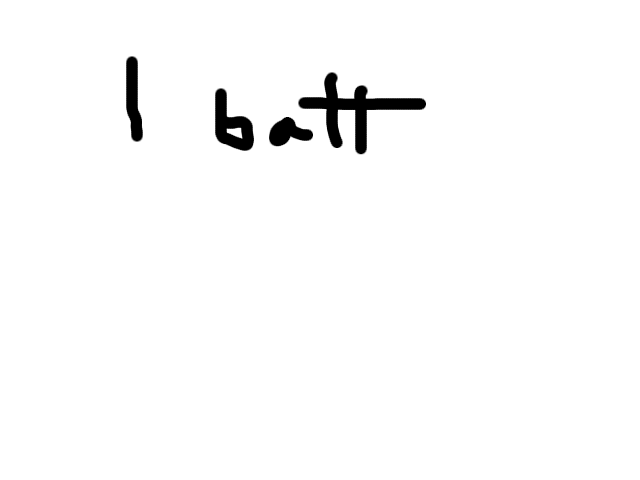
\includegraphics[width=0.4\textwidth]{fig/onebattery}
\caption{Eating \(1\) battery}
\end{figure}

\begin{figure}[h]
\label{fig:fivebatteries}
\centering
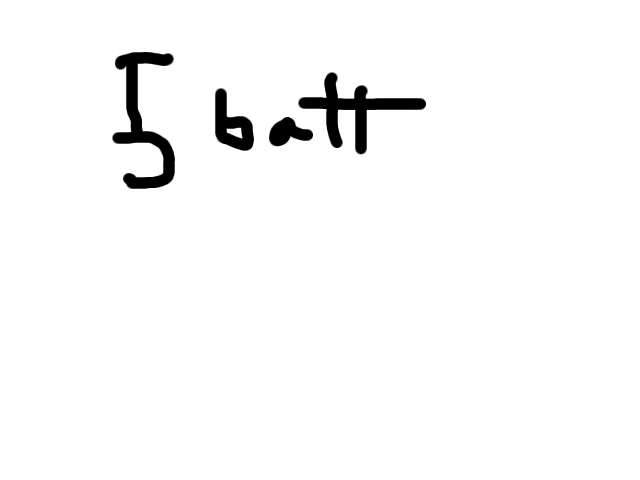
\includegraphics[width=0.4\textwidth]{fig/fivebatteries}
\caption{Eating \(5\) batteries}
\end{figure}

\begin{table}[h]
\label{tab:ssb}
\caption{Captain Falcon}
\centering
\begin{tabular}{r | l}
Falcons & Not Falcons\\
\hline
FALCON & KICK\\
FALCON & KICK\\
FALCON & PUNCH!!
\end{tabular}
\end{table}


\end{document}
\end{verbatim}
\normalsize

This is how appendices are included. In fact, they are written just like
regular chapters, and the \textbackslash appendix flag signals that following
chapters should be given letters (A, B, C...) instead of numbers (1, 2, 3...).

\chapter{Gotchas and Caveats}

\section{Introduction}

\texttt{uafthesis} is not perfect. It still has issues that you need to keep
in mind.

\section{List of Appendices Chicanery}

In an ideal world, \texttt{uafthesis} would write your appendices to the
list of appendices instead of the table of contents. This is currently a bug,
and will be fixed in the future.

The workaround is this:

\begin{enumerate}
\item After generating a pretty-much-done thesis, open up the .toc file. In
this case, the file is called ``example.toc.'' Also open up a corresponding
.loa file (``example.loa'').
\item Cut the lines that refer to appendices out of the .toc file and paste
them into the .loa file. Save both. Make sure the first line in the .loa
that adds "Page" above the pages column stays put.
\item \emph{Make backups of both files.} This is because \LaTeX will overwrite
the .toc file in the next step.
\item Compile (\texttt{pdflatex example}) \emph{exactly once.}
\end{enumerate}

\section{List of Other Materials}

A similar process applies to the List of Other Materials as well:

\begin{quotation}
{ \it ``If you add a pocket or anything else to your thesis (like a CD-ROM)
then you have to have one more List in the Table of Contents.  Follow
the exact same procedure as in step 14, but now you must add the
command:

\textbackslash listofothermaterials

Notice that this goes before the \textbackslash listofappendices.  The file that you
must edit is the thesis12.lom file.  You have to create this by hand.
It is simple.  Here is the example:

\textbackslash renewcommand\textbackslash @pnumwidth\{3.55em\}
\textbackslash contentsline \{section\}{\textbackslash numberline \{A\}CD-ROM of Thesis, Defense and Sandpile Code\}\{Pocket\}
\textbackslash renewcommand\textbackslash @pnumwidth\{1.55em\}

Again, once you save this and run latex once, it will be erased.  A
good habit is to make thesis12.lom.bak and thesis12.loa.bak so they
will always be there.  Then copy them to thesis12.lom and thesis12.loa
and run latex your final time.

I did the \textbackslash @pnumwidth stuff above because the word `Pocket' is wider
than is allowed for a page number.  So I changed it just for this one
line and then changed it back to what it was (as found in the
uafthesis2004.cls file).''\\
\hspace*{1in}---Ryan Woodard
\end{quotation}

I suspect that there's a better way to do this, but I haven't gotten that far
yet.

\section{Bibliography Listings}

If you use \texttt{chapterbib}, also use \texttt{tocbibind} to make sure that
your bibliographies show up in the Table of Contents.

\end{verbatim}
\normalsize

After inputting a few more pages, the chapters (separate documents) are all
included.

\small
\begin{verbatim}
\nocite{wikibook}
\bibliographystyle{agufull08}
\bibliography{thesis}
\end{verbatim}
\normalsize

This generates the bibliography. Note that the bibliography style is set to
\texttt{agufull08}. Generally, the graduate school isn't picky about 
bibliography style, as long as it's consistent. For geophysics papers (very
common at UAF), the AGU style is a great choice. It is included here, but may
also be found at AGU's web site.

\small
\begin{verbatim}
\appendix
\chapter{Extraneous Images and Tables}

\begin{figure}[h]
\label{fig:onebattery}
\centering
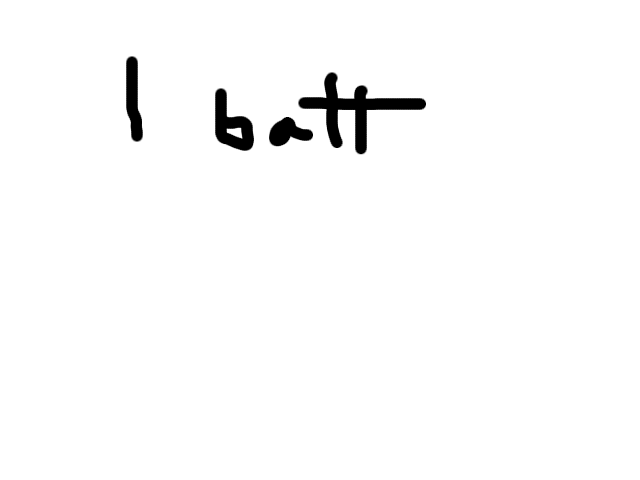
\includegraphics[width=0.4\textwidth]{fig/onebattery}
\caption{Eating \(1\) battery}
\end{figure}

\begin{figure}[h]
\label{fig:fivebatteries}
\centering
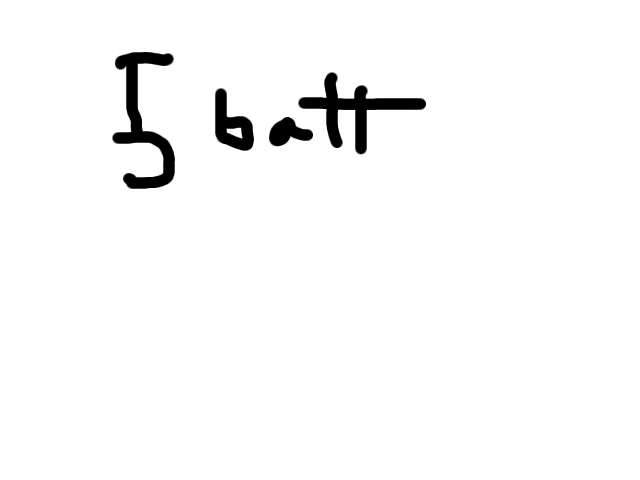
\includegraphics[width=0.4\textwidth]{fig/fivebatteries}
\caption{Eating \(5\) batteries}
\end{figure}

\begin{table}[h]
\label{tab:ssb}
\caption{Captain Falcon}
\centering
\begin{tabular}{r | l}
Falcons & Not Falcons\\
\hline
FALCON & KICK\\
FALCON & KICK\\
FALCON & PUNCH!!
\end{tabular}
\end{table}


\end{document}
\end{verbatim}
\normalsize

This is how appendices are included. In fact, they are written just like
regular chapters, and the \textbackslash appendix flag signals that following
chapters should be given letters (A, B, C...) instead of numbers (1, 2, 3...).

%     \chapter{Gotchas and Caveats}

\section{Introduction}

\texttt{uafthesis} is not perfect. It still has issues that you need to keep
in mind.

\section{List of Appendices Chicanery}

In an ideal world, \texttt{uafthesis} would write your appendices to the
list of appendices instead of the table of contents. This is currently a bug,
and will be fixed in the future.

The workaround is this:

\begin{enumerate}
\item After generating a pretty-much-done thesis, open up the .toc file. In
this case, the file is called ``example.toc.'' Also open up a corresponding
.loa file (``example.loa'').
\item Cut the lines that refer to appendices out of the .toc file and paste
them into the .loa file. Save both. Make sure the first line in the .loa
that adds "Page" above the pages column stays put.
\item \emph{Make backups of both files.} This is because \LaTeX will overwrite
the .toc file in the next step.
\item Compile (\texttt{pdflatex example}) \emph{exactly once.}
\end{enumerate}

\section{List of Other Materials}

A similar process applies to the List of Other Materials as well:

\begin{quotation}
{ \it ``If you add a pocket or anything else to your thesis (like a CD-ROM)
then you have to have one more List in the Table of Contents.  Follow
the exact same procedure as in step 14, but now you must add the
command:

\textbackslash listofothermaterials

Notice that this goes before the \textbackslash listofappendices.  The file that you
must edit is the thesis12.lom file.  You have to create this by hand.
It is simple.  Here is the example:

\textbackslash renewcommand\textbackslash @pnumwidth\{3.55em\}
\textbackslash contentsline \{section\}{\textbackslash numberline \{A\}CD-ROM of Thesis, Defense and Sandpile Code\}\{Pocket\}
\textbackslash renewcommand\textbackslash @pnumwidth\{1.55em\}

Again, once you save this and run latex once, it will be erased.  A
good habit is to make thesis12.lom.bak and thesis12.loa.bak so they
will always be there.  Then copy them to thesis12.lom and thesis12.loa
and run latex your final time.

I did the \textbackslash @pnumwidth stuff above because the word `Pocket' is wider
than is allowed for a page number.  So I changed it just for this one
line and then changed it back to what it was (as found in the
uafthesis2004.cls file).''\\
\hspace*{1in}---Ryan Woodard
\end{quotation}

I suspect that there's a better way to do this, but I haven't gotten that far
yet.

\section{Bibliography Listings}

If you use \texttt{chapterbib}, also use \texttt{tocbibind} to make sure that
your bibliographies show up in the Table of Contents.

%   \end{document}
% \end{verbatim}
% will process only the file \texttt{ch2.tex} as though the files
% \texttt{ch1.tex} and \texttt{ch3.tex} were also present. That is, all
% counters, especially the page and section numbers, as well as
% cross-referencing definitions, will function as if the whole document
% were processed. The trick is that each |\include|d file has it own
% \texttt{.aux} file containing these definitions, and they are all read
% in every time, even if the corresponding \texttt{.tex} file is not. The
% \texttt{.aux} files also contain the citation information for \btx,
% something that the \texttt{chapterbib} package exploits.
% 
% If |\usepackage{chapterbib}| has been given, the keys in each |\cite|
% and |\bibitem| command are associated with the current |\include|d file
% and are distinguished from the identical key in a different file. Each of
% these files must contain its own |\bibliography| and |\bibliographystyle|
% commands. One processes \btx\ on each file separately before processing
% it under \LaTeX\ (at least twice).
% 
% \subsubsection{Special Considerations for \thestyle\ and
%           \texttt{chapterbib}}
 
The order in which the \texttt{chapterbib} and \thestyle\ packages are loaded
is unimportant.

The \texttt{chapterbib} package provides an option \texttt{sectionbib}
that puts the bibliography in a |\section*| instead of |\chapter*|,
something that makes sense if there is a bibliography in each chapter.
This option will not work when \thestyle\ is also loaded; instead, add
the option to \thestyle. 
% (The \texttt{sectionbib} option can always be
% given, but it only has meaning for the \texttt{book} and \texttt{report}
% classes, or for classes derived from them.)

Every |\include|d file must contain its own
|\bibliography| command where the bibliography is to appear. The database
files listed as arguments to this command can be different in each file,
of course. However, what is not so obvious, is that each file must also
contain a |\bibliographystyle| command, \emph{preferably with the same
style  argument}. 
% If different bibliography styles are specified for
% different files, then the preprogrammed citation style (punctuation and
% citation mode) will be that of the first bibliography style given. The
% preprogrammed citation styles can only be changed in the preamble (see
% Section~\ref{sec:priority}), something that guarantees a uniform style
% for the entire document.\relax
%   \footnote{It would be relatively easy to allow changes in style anywhere
%   in the document, but this strikes me as bad policy. However, it is
%   provided for with the \texttt{docstrip} option \texttt{nopreonly}.}
% 
% \iffalse
%</notes>
% \fi
%
% \subsection{Sorting and Compressing Numerical Citations}
% \label{sec:sort}
% 
% Another package by Donald Arseneau, \texttt{cite.sty}, reimplements the
% entire (numerical) citation system such that one can control the
% punctuation and citation format, all of which is done by \thestyle\ as
% well. However, it also can sort and compress numerical citations,
% something that is required by some journals. 
% 
% What this means is that when multiple citations are given with a single
% |\cite| command, the normal order of the numbers is in the sequence
% given. This is usually a wild list of numbers, such as [4,2,8,3]. With
% the \texttt{cite} package, this list becomes [2--4,8].
% 
% It is impossible to make the \texttt{cite} and \thestyle\ packages
% compatible, since both reimplement |\cite| from scratch. Instead, I have
% taken over some of the coding from \texttt{cite.sty}, modifying it for 
% \thestyle{}. This coding is activated by including one of the options 
% \texttt{sort} or \texttt{sort\&compress} in the |\usepackage| command. 
% 
% For author--year citations, the option \texttt{sort} orders the citations in 
% a single |\citep| or |\citet| command into the sequence in which they appear 
% in the list of references. This is normally alphabetical first, year second. 
% This should avoid citations of the type: ``James et~al.\ (1994b,a)''. For 
% author--year mode, the \texttt{sort\&compress} option is identical to 
% \texttt{sort}. 
% 
% \iffalse
%<*notes>
\head{Sorting and compressing citations}
Do not use the \texttt{cite} package with \thestyle; rather use one of the 
options \texttt{sort} or \texttt{sort\&compress}.

These also work with author--year citations, making multiple citations appear 
in their order in the reference list. 

%</notes>
% \fi
% 
% \subsection{Long Author List on First Citation}\label{sec:long}
% 
% A feature that has often been requested by otherwise happy users of 
% \thestyle\ is one that is found in the \texttt{harvard} package as 
% standard: with the first citation of any reference, the full author list is 
% printed, and afterwards only the abbreviated list. One can control this 
% with |\citet*| for the first citation, and |\citet| or |\citep| thereafter. 
% However, the automatic feature is very desired. 
% 
% This can be activated with the option 
% \texttt{longnamesfirst}.
% 
% \iffalse
%<*notes>
\head{Long author list on first citation}
Use option \texttt{longnamesfirst} to have first citation automatically give 
the full list of authors.

Suppress this for certain citations with |\shortcites{|\emph{key-list}|}|,
given before the first citation.

%</notes>
% \fi
%
% \DescribeMacro{\shortcites}
% Some references have so many authors that you want to suppress the 
% automatic long list only for them. In this case, issue
% \begin{quote}
%   |\shortcites|\marg{key-list}
% \end{quote}
% before the first citations, and those included in \emph{key-list} will have 
% a short list on their first citation. 
%
% Full author lists can still be forced at any time with the starred 
% variants.
% 
% \section{Numerical Citations with Author--Year Styles}\label{sec:6.0}
% 
% It is possible to produce numerical citations with any author-year 
% \texttt{.bst} file, with minimal change to the text. The commands |\citet| 
% and |\citep| will produce sensible results in both modes, without any special 
% editing. Obviously, the opposite is not possible; a \texttt{.bst} file 
% intended for numerical citation can never produce author--year citations, 
% simply because the information is not transferred to the auxiliary file.
% 
% \subsection{Selecting Numerical Mode}
% By default, \thestyle{} is in author--year mode. This can be changed by
% \begin{enumerate}
%   \item selecting a numerical bibliography style with predefined
%         citation style, defined either in the package or in the local
%         configuration file;
%         
%   \item giving options \texttt{numbers} or \texttt{super} to the
%         |\usepackage| command;
% 
%   \item issuing |\bibpunct| with the 4th mandatory argument set to \texttt{n}
%         or \texttt{s};
% 
%   \item issuing |\citestyle| with the name of a predefined numerical
%         bibliography style.
% \end{enumerate}
% The methods are listed in order of increasing priority. 
% 
% The \thestyle{} package will automatically switch to numerical mode if
% any one of the |\bibitem| entries fails to conform to the possible
% author--year formats. There is no way to override this, since such an
% entry would cause trouble in the author--year mode.
% 
% There are certain special `numerical' styles, like that of the standard
% \texttt{alpha.bst}, which include a non-numerical label in place of the
% number, in the form
% \begin{quote} |\bibitem[ABC95]{able95}| \end{quote}
% As far as \thestyle\ is concerned, this label does not conform to the
% author--year possibilities and is therefore considered to be numerical.
% The citation mode switches to numerical, and |\cite{able95}| prints
% [ABC95].
% 
% See however, the end of Section~\ref{sec:yearless} for another possibility.
% The above result can be achieved with
% \begin{quote} |\bibitem[ABC95()]{able95}| \end{quote}
%
% \section{Local Configuration}
% For \LaTeXe, it is possible to add a local configuration file
% \thestyle\texttt{.cfg}, which is read in, if it exists, at
% the end of the package. It may thus contain coding to supecede that in
% the package, although its main purpose is to allow the user to add his
% own |\bibstyle@|\textit{bst} definitions to couple citation punctuation
% with local bibliography styles.
%
% \iffalse
%<*notes>
\head{Local configuration}
Any local recoding or definitions can be put in \thestyle\texttt{.cfg} which 
is read in after the main package file.

%</notes>
% \fi
% 
% \section{Options with \LaTeXe}\label{sec:opts}
% One of the new features of \LaTeXe{} is \emph{options} for the packages,
% in the same way as main styles (now called \emph{classes}) can take
% options. This package is now installed with
% \begin{quote}
% |\documentclass[..]{...}|\\
% |\usepackage[|\emph{options}|]{|\thestyle|}|
% \end{quote}
% \iffalse
%<*notes>
\head{Options that can be added to \texttt{\char`\\ usepackage}}
% \fi
% The options available provide another means of specifying the
% punctuation for citations:
\begin{description}
\item[\ttfamily round] (default) for round parentheses;
\item[\ttfamily square] for square brackets;
\item[\ttfamily curly] for curly braces;
\item[\ttfamily angle] for angle brackets;
\item[\ttfamily colon] (default) to separate multiple citations with
     colons;
\item[\ttfamily comma] to use commas as separaters;
\item[\ttfamily authoryear] (default) for author--year citations;
\item[\ttfamily numbers] for numerical citations;
\item[\ttfamily super] for superscripted numerical citations, as in
     \textsl{Nature};
\item[\ttfamily sort] orders multiple citations into the sequence in 
     which they appear in the list of references;
\item[\ttfamily sort\&compress] as \texttt{sort} but in addition multiple
     numerical citations are compressed if possible (as 3--6, 15);
\item[\ttfamily longnamesfirst] makes the first citation of any reference 
     the equivalent of the starred variant (full author list) and subsequent 
     citations normal (abbreviated list);
\item[\ttfamily sectionbib] redefines |\thebibliography| to issue
     |\section*| instead of |\chapter*|; valid only for classes with a
     |\chapter| command; to be used with the \texttt{chapterbib} package;
\item[\ttfamily nonamebreak] keeps all the authors' names in a citation on 
     one line; causes overfull hboxes but helps with some \texttt{hyperref} 
     problems.
\end{description}
% \iffalse
%</notes>
% \fi
% 
% If any of the formatting options are selected, the predefined citation 
% styles in the commands |\bibstyle@|\textit{bst} will be no longer be 
% effective. If either |\bibpunct| or |\citestyle| is given in the preamble, 
% the above punctuation options will no longer hold. 
% 
% \section{As Module to Journal-Specific Styles}
% Although \thestyle{} is meant to be an all-purpose bibliographic style
% \emph{package}, it may also be incorporated as a module to other 
% packages for specific journals. In this case, many of the general features may
% be left off. This is allowed for with \texttt{docstrip} options that not
% only leave off certain codelines, but also include extra ones. So far,
% options exist for 
% \begin{description}
% \item[\ttfamily subpack] produces a basic version with author--year only,
% fixed citation punctuation, no |\bibpunct| nor |\citestyle| nor 
% predefined styles;
% \item[\ttfamily subpack,egs] for journals of the \textsl{European Geophysical
% Society}, in particular \textsl{Nonlinear Processes in Geophysics};
% \item[\ttfamily subpack,agu] for \textsl{American Geophysical Union} journals.
% \end{description}
% The \texttt{subpack} option must always be used with \texttt{package}.
% 
% Previous options \texttt{jgr} and \texttt{grl} have become obsolete due
% to revisions in these journals; they have been replaced by the more
% general \texttt{agu} option.
% 
% \section{Reference Sheet}
% 
% A summarization of the main points on using \thestyle\ can be obtained by 
% \LaTeX{}ing the file \texttt{natnotes.tex}, which is extracted from the main 
% source file \thestyle\texttt{.dtx} with the \texttt{docstrip} option 
% \texttt{notes}. This is intended to act as a handy reference sheet.
% 
% This file should be extracted automatically by the supplied installation file,
% \thestyle\texttt{.ins}.
% 
%^^A The following is a summary that goes into the .sty file
%^^A It is not printed in the documentation, since the Reference Sheet exists
% \iffalse  
%<*package&!subpack>
 % This package reimplements the LaTeX \cite command to be used for various
 % citation styles, both author-year and numerical. It accepts BibTeX
 % output intended for many other packages, and therefore acts as a 
 % general, all-purpose citation-style interface.
 %
 % With standard numerical .bst files, only numerical citations are
 % possible. With an author-year .bst file, both numerical and
 % author-year citations are possible.
 %
 % If author-year citations are selected, \bibitem must have one of the
 %   following forms:
 %   \bibitem[Jones et al.(1990)]{key}...
 %   \bibitem[Jones et al.(1990)Jones, Baker, and Williams]{key}...
%<*apalike|all>
 %   \bibitem[Jones et al., 1990]{key}...
%</apalike|all>
%<*newapa|chicago|all>
 %   \bibitem[\protect\citeauthoryear{Jones, Baker, and Williams}{Jones
 %       et al.}{1990}]{key}...
 %   \bibitem[\protect\citeauthoryear{Jones et al.}{1990}]{key}...
%</newapa|chicago|all>
%<*astron|all>
 %   \bibitem[\protect\astroncite{Jones et al.}{1990}]{key}...
%</astron|all>
%<*authordate|all>
 %   \bibitem[\protect\citename{Jones et al., }1990]{key}...
%</authordate|all>
%<*harvard|all>
 %   \harvarditem[Jones et al.]{Jones, Baker, and Williams}{1990}{key}...
%</harvard|all>
 %   
 % This is either to be made up manually, or to be generated by an 
 % appropriate .bst file with BibTeX.
 %                            Author-year mode     ||   Numerical mode
 % Then, \citet{key}  ==>>  Jones et al. (1990)    ||   Jones et al. [21]
 %       \citep{key}  ==>> (Jones et al., 1990)    ||   [21]
 % Multiple citations as normal:
 % \citep{key1,key2}  ==>> (Jones et al., 1990; Smith, 1989) || [21,24]
 %                           or  (Jones et al., 1990, 1991)  || [21,24]
 %                           or  (Jones et al., 1990a,b)     || [21,24]
 % \cite{key} is the equivalent of \citet{key} in author-year mode
 %                         and  of \citep{key} in numerical mode
 % Full author lists may be forced with \citet* or \citep*, e.g.
 %       \citep*{key}      ==>> (Jones, Baker, and Williams, 1990)
 % Optional notes as:
 %   \citep[chap. 2]{key}    ==>> (Jones et al., 1990, chap. 2)
 %   \citep[e.g.,][]{key}    ==>> (e.g., Jones et al., 1990)
 %   \citep[see][pg. 34]{key}==>> (see Jones et al., 1990, pg. 34)
 %  (Note: in standard LaTeX, only one note is allowed, after the ref.
 %   Here, one note is like the standard, two make pre- and post-notes.)
 %   \citealt{key}          ==>> Jones et al. 1990
 %   \citealt*{key}         ==>> Jones, Baker, and Williams 1990
 %   \citealp{key}          ==>> Jones et al., 1990
 %   \citealp*{key}         ==>> Jones, Baker, and Williams, 1990
 % Additional citation possibilities (both author-year and numerical modes)
 %   \citeauthor{key}       ==>> Jones et al.
 %   \citeauthor*{key}      ==>> Jones, Baker, and Williams
 %   \citeyear{key}         ==>> 1990
 %   \citeyearpar{key}      ==>> (1990)
 %   \citetext{priv. comm.} ==>> (priv. comm.)
 % Note: full author lists depends on whether the bib style supports them;
 %       if not, the abbreviated list is printed even when full requested.
 %
 % For names like della Robbia at the start of a sentence, use
 %   \Citet{dRob98}         ==>> Della Robbia (1998)
 %   \Citep{dRob98}         ==>> (Della Robbia, 1998)
 %   \Citeauthor{dRob98}    ==>> Della Robbia
 %
%<*!209>
 % 
 % Citation aliasing is achieved with
 %   \defcitealias{key}{text}
 %   \citetalias{key}  ==>> text
 %   \citepalias{key}  ==>> (text)
%</!209>
 %
 % Defining the citation style of a given bib style:
%<!nopreonly> % Use \bibpunct (in the preamble only) with 6 mandatory arguments:
%<nopreonly> % Use \bibpunct (anywhere in the text) with 6 mandatory arguments:
 %    1. opening bracket for citation
 %    2. closing bracket
 %    3. citation separator (for multiple citations in one \cite)
 %    4. the letter n for numerical styles, s for superscripts
 %        else anything for author-year
 %    5. punctuation between authors and date
 %    6. punctuation between years (or numbers) when common authors missing
 % One optional argument is the character coming before post-notes. It
 %   appears in square braces before all other arguments. May be left off.
 % Example (and default) \bibpunct[, ]{(}{)}{;}{a}{,}{,}
 % 
 % To make this automatic for a given bib style, named newbib, say, make
 % a local configuration file, natbib.cfg, with the definition
 %   \newcommand{\bibstyle@newbib}{\bibpunct...}
 % Then the \bibliographystyle{newbib} will cause \bibstyle@newbib to 
 % be called on THE NEXT LATEX RUN (via the aux file).
 %
%<!nopreonly> % Such preprogrammed definitions may be invoked in the text (preamble only)
%<nopreonly> % Such preprogrammed definitions may be invoked anywhere in the text
 %  by calling \citestyle{newbib}. This is only useful if the style specified
 %  differs from that in \bibliographystyle.
 %
%<*!209>
 % With \citeindextrue and \citeindexfalse, one can control whether the
 % \cite commands make an automatic entry of the citation in the .idx
 % indexing file. For this, \makeindex must also be given in the preamble.
 %
 % LaTeX2e Options: (for selecting punctuation)
 %   round  -  round parentheses are used (default)
 %   square -  square brackets are used   [option]
 %   curly  -  curly braces are used      {option}
 %   angle  -  angle brackets are used    <option>
 %   colon  -  multiple citations separated by colon (default)
 %   comma  -  separated by comma
 %   authoryear - selects author-year citations (default)
 %   numbers-  selects numerical citations
 %   super  -  numerical citations as superscripts
 %   sort   -  sorts multiple citations according to order in ref. list
 %   sort&compress   -  like sort, but also compresses numerical citations
 %   longnamesfirst  -  makes first citation full author list
 %   sectionbib - puts bibliography in a \section* instead of \chapter*
 % Punctuation so selected dominates over any predefined ones.
 % LaTeX2e options are called as, e.g.
 %        \usepackage[square,comma]{natbib}
%</!209>
 % LaTeX the source file natbib.dtx to obtain more details
%<!209> % or the file natnotes.tex for a brief reference sheet.
 %-----------------------------------------------------------
%</package&!subpack>
% \fi
% 
% \section{Options with \texttt{docstrip}}
% The source \texttt{.dtx} file is meant to be processed with
% \texttt{docstrip}, for which a number of options are available:
% \begin{description}
% \item[\ttfamily all] includes all of the other interfaces;
%
% \item[\ttfamily apalike] allows interpretation of minimal \texttt{apalike} 
%    form of |\bibitem|;
%
% \item[\ttfamily newapa] allows |\citeauthoryear| to be in the optional 
%    argument of |\bibitem| along with the punctuation commands of 
%    \texttt{newapa.sty};
%
% \item[\ttfamily chicago] is the same as \texttt{newapa};
%
% \item[\ttfamily harvard] includes interpretation of |\harvarditem|;
%
% \item[\ttfamily astron] allows |\astroncite| to appear in the optional 
%    argument of |\bibitem|;
%
% \item[\ttfamily authordate] adds the syntax of the |\citename| command.
%
% \end{description}
%
% This package file is intended to act as a module for other class files
% written for specific journals, in which case the flexible
% |\bibstyle@|{\em bst\/} commands are not wanted. Punctuation and
% other style features are to be rigidly fixed. These journal options are
% \begin{description}
% \item[\ttfamily agu] for journals of the \textsl{American Geophysical
%   Union};
%
% \item[\ttfamily egs] for journals of the \textsl{European Geophysical 
%   Society}, in particular \textsl{Nonlinear Processes in Geophysics}.
%
% \end{description}
%
% The remaining options are:
% \begin{description}
% \item[\ttfamily package] to produce a \texttt{.sty} package file with most
%     comments removed;
% 
% \item[\ttfamily 209] (together with \texttt{package}) for a style option 
%     file that will run under the older \LaTeX~2.09;
% 
% \item[\ttfamily subpack] (together with \texttt{package}) for coding that 
%     is to be included inside a larger package; even more comments are 
%     removed, as well as \LaTeXe{} option handling and identification;
%     produces a basic \thestyle\ package for author--year only, fixed
%     citation style (punctuation);
%
% \item[\ttfamily notes] extracts a summary of usage to be used as a
%     reference sheet; the resulting file is to be \LaTeX{}ed;
%
% \item[\ttfamily nopreonly] allows |\citestyle| and |\bibpunct| to be
%     called anywhere in the text; this is considered possibly useful
%     with the \texttt{chapterbib} package where different chapters might 
%     have different bibliography and citation styles; is only provided 
%     in case I change my mind about this feature, but for now I 
%     refuse to implement it;
%
% \item[\ttfamily driver] to produce a driver \texttt{.drv} file that will
%     print out the documentation under \LaTeXe. The documentation cannot
%     be printed under \LaTeX~2.09.
% 
% \end{description}
% The source file \texttt{\filename.dtx} is itself a driver file and can
% be processed directly by \LaTeXe.
%
% \iffalse
%<notes>\end{document}
% \fi
%
% \StopEventually{\PrintIndex\PrintChanges}
% 
% \section{The Coding}
% This section presents and explains the actual coding of the macros.
% It is nested between |%<*package>| and |%</package>|, which
% are indicators to \texttt{docstrip} that this coding belongs to the package 
% file.
%
% The \texttt{docstrip} option |<subpack>| should only be called if the
% coding is to be included as part of another package, in which case the 
% announcement text and \LaTeXe{} options are suppressed.
%
% An alternative version of this coding is provided for running as a 
% style file under \LaTeX~2.09. Code lines belonging to this are
% indicated with guard |<209>|; those for LaTeXe{} only with |<!209>|.
%
% With \LaTeX\ release from \texttt{1995/12/01}, |\cite| is made robust, 
% something that I have adopted as well.
% 
% Another change in the above release is that 
% |\G@refundefinedtrue|\footnote{In fact, it was only proposed to be 
%    removed, but because several packages, including this one, were 
%    adversely affected, the name was retained for the new coding.}
% and the |\if@openbib| flag have been removed.
% New, more effective, and compact, coding has replaced them. Rather than
% relying on the kernel coding, I make \thestyle\ more
% self-reliant. 
% 
% \subsection{Test for Specific Journals}
% This package should not be loaded with the specific journal packages that
% already include it; it is superfluous and can lead to contradictions.
%    \begin{macrocode}
%<*package>
%<*!209&!subpack>
\@ifclassloaded{aguplus}{\PackageError{natbib}
  {The aguplus class already includes natbib coding,\MessageBreak
   so you should not add it explicitly}
  {Type <Return> for now, but then later remove\MessageBreak
   the command \protect\usepackage{natbib} from the document}
  \endinput}{}
\@ifclassloaded{nlinproc}{\PackageError{natbib}
  {The nlinproc class already includes natbib coding,\MessageBreak
   so you should not add it explicitly}
  {Type <Return> for now, but then later remove\MessageBreak
   the command \protect\usepackage{natbib} from the document}
  \endinput}{}
\@ifclassloaded{egs}{\PackageError{natbib}
  {The egs class already includes natbib coding,\MessageBreak
   so you should not add it explicitly}
  {Type <Return> for now, but then later remove\MessageBreak
   the command \protect\usepackage{natbib} from the document}
  \endinput}{}
%</!209&!subpack>
%    \end{macrocode}
%
% \subsection{Selecting Citation Punctuation and Other Modifications}
% \begin{macro}{\bibstyle@xxx}
% \changes{5.3}{1994 Sep 13}{Add \texttt{agsm} and \texttt{dcu} punctuation 
%    styles from \texttt{harvard} series}
% We begin by defining a number of punctuation styles for specific
% author--year \texttt{.bst} files that I use. 
% They are placed here, near the beginning, so that another
% user can easily find them to add his own. Some comments remain in the
% stripped version too.
%    \begin{macrocode}
%<*!subpack>
 % Define citation punctuation for some author-year styles
 % One may add and delete at this point
%<!209> % Or put additions into local configuration file natbib.cfg
\newcommand\bibstyle@chicago{\bibpunct{(}{)}{;}{a}{,}{,}}
\newcommand\bibstyle@named{\bibpunct{[}{]}{;}{a}{,}{,}}
\newcommand\bibstyle@agu{\bibpunct{[}{]}{;}{a}{,}{,~}}%Amer. Geophys. Union
\newcommand\bibstyle@egs{\bibpunct{(}{)}{;}{a}{,}{,}}%Eur. Geophys. Soc.
%<*all|harvard>
\newcommand\bibstyle@agsm{\bibpunct{(}{)}{,}{a}{}{,}\gdef\harvardand{\&}}
\newcommand\bibstyle@kluwer{\bibpunct{(}{)}{,}{a}{}{,}\gdef\harvardand{\&}}
\newcommand\bibstyle@dcu{\bibpunct{(}{)}{;}{a}{;}{,}\gdef\harvardand{and}}
%</all|harvard>
%    \end{macrocode}
% 
% Here give the explicit punctuation for the specific journals; their
% coding need not contain the punctuation macros |\bibpunct| and
% |\bibstyle@xxx| since the punctuation is fixed for them.
%
% Activate citation sorting for the journals.
% \changes{6.8b}{1998 July 2}{Turn off sorting for AGU and EGS}
%    \begin{macrocode}
\newcommand\bibstyle@aa{\bibpunct{(}{)}{;}{a}{}{,}} %Astronomy & Astrophysics
\newcommand\bibstyle@pass{\bibpunct{(}{)}{;}{a}{,}{,}}%Planet. & Space Sci
\newcommand\bibstyle@anngeo{\bibpunct{(}{)}{;}{a}{,}{,}}%Annales Geophysicae
\newcommand\bibstyle@nlinproc{\bibpunct{(}{)}{;}{a}{,}{,}}%Nonlin.Proc.Geophys.
%</!subpack>
%<agu>\newcommand\NAT@open{[} \newcommand\NAT@close{]} 
%<agu>\newcommand\NAT@sep{;} \newcommand\NAT@cmt{, }
%<agu>\newcommand\NAT@aysep{,} \newcommand\NAT@yrsep{,~}
%<agu|egs>\def\NAT@sort{0}
%<egs>\newcommand\NAT@open{(} \newcommand\NAT@close{)} 
%<egs>\newcommand\NAT@sep{;} \newcommand\NAT@cmt{, }
%<egs>\newcommand\NAT@aysep{,} \newcommand\NAT@yrsep{,}
%    \end{macrocode}
% 
% \changes{6.5}{1997 Jan 30}{Fix \texttt{esa} style for new note system}
% \changes{7.0}{1999 May 7}{Fix \texttt{esa} style again}
% Next, the same thing is done for some numerical styles. A major
% difference here is that the |\@biblabel| and |\@cite| commands must also
% be redefined in many cases. These redefinitions must be made with the
% |\gdef| (global definition) command.
%    \begin{macrocode}
%<*!subpack>
 % Define citation punctuation for some numerical styles
\newcommand\bibstyle@cospar{\bibpunct{/}{/}{,}{n}{}{}%
     \gdef\NAT@biblabelnum##1{##1.}}
\newcommand\bibstyle@esa{\bibpunct{(Ref.~}{)}{,}{n}{}{}%
     \gdef\NAT@biblabelnum##1{##1.\hspace{1em}}}
\newcommand\bibstyle@nature{\bibpunct{}{}{,}{s}{}{\textsuperscript{,}}%
     \gdef\NAT@biblabelnum##1{##1.}}
%    \end{macrocode}
% 
% Finally, the standard \LaTeX{} (numerical) citation styles are included
%  along with their \thestyle\ modifications (author--year).
%    \begin{macrocode}
 % The standard LaTeX styles
\newcommand\bibstyle@plain{\bibpunct{[}{]}{,}{n}{}{,}}
\let\bibstyle@alpha=\bibstyle@plain
\let\bibstyle@abbrv=\bibstyle@plain
\let\bibstyle@unsrt=\bibstyle@plain
 % The author-year modifications of the standard styles
\newcommand\bibstyle@plainnat{\bibpunct{[}{]}{,}{a}{,}{,}}
\let\bibstyle@abbrvnat=\bibstyle@plainnat
\let\bibstyle@unsrtnat=\bibstyle@plainnat
%    \end{macrocode}
% \end{macro}
% 
% \subsection{\LaTeXe{} Options}
% \begin{macro}{\ifNAT@numbers}
% \changes{5.5}{1995 Mar 21}{Add flag for switching between cite styles}
% \begin{macro}{\ifNAT@super}
% \changes{5.5}{1995 Mar 21}{Add flag for switching between cite styles}
% Two flags are used to keep track of the citation style. The flag
% |\ifNAT@numbers| is \meta{false} by default (author--year) and switches
% to \meta{true} for numerical citations. The flag |\ifNAT@super| indicates
% if the numerical citation is to be done with superscripts.
%    \begin{macrocode}
\newif\ifNAT@numbers \NAT@numbersfalse
\newif\ifNAT@super \NAT@superfalse
%</!subpack>
%    \end{macrocode}
% \end{macro}\end{macro}
%
% \begin{macro}{\DeclareOption}
% \changes{5.0}{1994 May 18}{Add \LaTeXe{} options.}
% \changes{5.3}{1994 Sep 13}{Add options \texttt{angle} and \texttt{curly}}
% \changes{6.0}{1995 Sep 6}{Add option \texttt{bibstyle}}
% \changes{6.0}{1995 Sep 6}{Execute \texttt{nobibstyle} with all options}
% \changes{6.1}{1995 Nov 27}{Add option \texttt{openbib}}
% \changes{6.4}{1996 Sep 1}{Add option \texttt{sectionbib}}
% \changes{6.4}{1996 Sep 13}{Add option \texttt{sort}}
% \changes{6.7}{1997 Jul 14}{Add option \texttt{longnamesfirst}}
% \changes{6.8c}{1998 Jul 14}{Add option \texttt{nonamebreak}}
% For \LaTeXe, we can define some options to be used with the |\usepackage|
% command that loads the \thestyle{} package. These are an additional means
% of specifying the citation punctuation and scheme.
% 
% The standard option \texttt{openbib} is also defined here so that its
% behaviour is entirely under my control. Relying on the standard classes
% can lead to trouble.
%    \begin{macrocode}
%<*!subpack&!209>
\DeclareOption{numbers}{\NAT@numberstrue
   \ExecuteOptions{square,comma,nobibstyle}}
\DeclareOption{super}{\NAT@supertrue\NAT@numberstrue
   \renewcommand\NAT@open{}\renewcommand\NAT@close{}
   \ExecuteOptions{nobibstyle}}
\DeclareOption{authoryear}{\NAT@numbersfalse
   \ExecuteOptions{round,colon,bibstyle}}
\DeclareOption{round}{%
      \renewcommand\NAT@open{(} \renewcommand\NAT@close{)}
   \ExecuteOptions{nobibstyle}}
\DeclareOption{square}{%
      \renewcommand\NAT@open{[} \renewcommand\NAT@close{]}
   \ExecuteOptions{nobibstyle}}
\DeclareOption{angle}{%
      \renewcommand\NAT@open{$<$} \renewcommand\NAT@close{$>$}
   \ExecuteOptions{nobibstyle}}
\DeclareOption{curly}{%
      \renewcommand\NAT@open{\{} \renewcommand\NAT@close{\}}
   \ExecuteOptions{nobibstyle}}
\DeclareOption{comma}{\renewcommand\NAT@sep{,}
   \ExecuteOptions{nobibstyle}}
\DeclareOption{colon}{\renewcommand\NAT@sep{;}
   \ExecuteOptions{nobibstyle}}
\DeclareOption{nobibstyle}{\let\bibstyle=\@gobble}
\DeclareOption{bibstyle}{\let\bibstyle=\@citestyle}
\newif\ifNAT@openbib \NAT@openbibfalse
\DeclareOption{openbib}{\NAT@openbibtrue}
\DeclareOption{sectionbib}{\def\NAT@sectionbib{on}}
\def\NAT@sort{0}
\DeclareOption{sort}{\def\NAT@sort{1}}
\DeclareOption{sort&compress}{\def\NAT@sort{2}}
\@ifpackageloaded{cite}{\PackageWarningNoLine{natbib}
  {The `cite' package should not be used\MessageBreak
   with natbib. Use option `sort' instead}\ExecuteOptions{sort}}{}
\newif\ifNAT@longnames\NAT@longnamesfalse
\DeclareOption{longnamesfirst}{\NAT@longnamestrue}
\DeclareOption{nonamebreak}{\def\NAT@nmfmt#1{\mbox{\NAT@up#1}}}
%</!subpack&!209>
\def\NAT@nmfmt#1{{\NAT@up#1}}
%    \end{macrocode}
% Before version~6.0, the punctuation options had the lowest priority,
% being overridden by any |\bibstyle@|\textit{bst} command. It was necessary
% to add the option \texttt{nobibstyle} to make them effective. Now this
% option is automatically executed whenever a punctuation option is chosen.
% The reason is that \texttt{nobibstyle} is either superfluous (no
% predefined citation style is present) or always necessary to make the
% other options meaningful. 
% 
% It seems to be better practice to make any explicit choices to have
% higher priority over implicit ones.
% 
% The option \texttt{bibstyle} reactivates the predefined commands, just in
% case this is needed, as it is for the option \texttt{authoryear}. This
% leaves the predefined styles functioning, since it does not really
% determine the citation style, but rather establishes a default which may
% be overwritten by a prestored one.  For this reason, this option must be
% defined very early so that any explicit punctuation options overwrite the
% defaults. (Options are executed in the order defined.)
% 
% \end{macro}
%
% \subsection{Selecting Citation Punctuation and Other Modifications}
% \begin{macro}{\bibstyle}
% \changes{5.4}{1994 Nov 24}{Move \cs{ProcessOptions} to after definition
%    of \cs{bibstyle}}
% The pre-defined punctuation styles are associated with particular
% \texttt{.bst} files. This is implemented by means of the standard
% |\bibliographystyle| command that specifies the name of the \texttt{.bst}
% file that is to be used by \btx. Some \LaTeX{} manuals erroneously state
% that this command must be issued prior to any |\cite| commands. If that
% were the case, the task of invoking the style definitions would be much
% easier, for they certainly must be issued before the first |\cite|.
% However, I have always called |\bibliographystyle| together with
% |\bibliography|, well after all |\cite| commands. 
% 
% In fact, all that |\bibliographystyle|\marg{bst} does is to write
% |\bibstyle|\marg{bst} to the auxiliary file. This file, and all its
% contents, will be read in at the beginning of the next \LaTeX{} run; to
% be precise, it is read in by |\begin{document}|. The command |\bibstyle| is
% then executed at that point on the next run. However, it is 
% defined to do nothing more than to swallow up its argument! In other
% words, the combination |\bibliographystyle| and |\bibstyle| do absolutely
% nothing to the \LaTeX{} runs. In fact, |\bibstyle| is a command for
% \btx{} alone.
% 
% I have taken advantage of this to redefine |\bibstyle| to execute the
% \texttt{bst}-specific definitions. This definition is made here before
% |\ExecuteOptions| so that options may make use of it; the option
% \texttt{nobibstyle} turns it off, for example.
%    \begin{macrocode}
%<*!subpack>
\renewcommand\bibstyle[1]{\@ifundefined{bibstyle@#1}{\relax}
     {\csname bibstyle@#1\endcsname}}
%    \end{macrocode}
% This is executed only when the auxiliary file is read in, and that is
% when |\begin{document}| is issued. Thus this is well before any |\cite|
% commands. It is for this reason that any definitions in the
% |\bibstyle@xxx| commands must be global.
% 
% A minor problem arises in that the auxiliary file is read in a second
% time, at the end of the run, to check whether any labels have changed. 
% Sometimes, re-executing the |\bibstyle@xxx| command at this point
% produces error messages. To avoid this, |\bibstyle| is reset to its
% normal, do-nothing, definition after |\begin{document}|.
% 
% \LaTeXe{} provides a better way of adding commands to |\document|,
% which is then exploited here. Paradoxically, the problem with re-reading
% the auxiliary file does not seem to arise for this version.
% 
% (|\NAT@set@cites| must also be executed at the start of the document; for
% \LaTeXe, this is added later when the macro is defined.)
%    \begin{macrocode}
%<*209>
\let\ori@document=\document
\renewcommand\document{\ori@document\global\let\bibstyle=\@gobble 
  \NAT@set@cites}
%</209>
%<!209>\AtBeginDocument{\global\let\bibstyle=\@gobble}
%    \end{macrocode}
% \end{macro}
% 
% \begin{macro}{\citestyle}
% \changes{5.4}{1995 Feb 03}{Add macro}
% \changes{5.5}{1995 Mar 24}{Make preamble only}
% To allow one to invoke preprogrammed punctuation styles that are
% different from the name of the bibliography style specified by
% |\bibliographystyle|, call |\citestyle| in the preamble. This then
% deactivates |\bibstyle| so that any preprogrammed punctuations become
% ineffective.
% 
% This, and all other punctuation (citation style) declarations, may only
% be used in the preamble, as of version 5.5. (Previously they could only
% be used after the preamble, but the preamble is more logical.)
%    \begin{macrocode}
\let\@citestyle\bibstyle
\newcommand\citestyle[1]{\@citestyle{#1}\let\bibstyle\@gobble}
%<!209&!nopreonly>\@onlypreamble{\citestyle}\@onlypreamble{\@citestyle}
%    \end{macrocode}
% \end{macro}
%
% \begin{macro}{\bibpunct}
% \changes{5.4}{1994 Nov 24}{Add superscript style of citations}
% \changes{5.5}{1995 Mar 21}{Use flags to select citation style}
% \changes{5.5}{1995 Mar 24}{Make preamble only}
% \changes{6.0}{1995 Sep 6}{Sets \cs{bibstyle} to \cs{@gobble}}
% \changes{6.0}{1995 Sep 6}{Declare \cs{NAT@numbersfalse} before testing 4th
%      argument}
% \changes{6.0}{1995 Sep 19}{Add optional argument for \cs{NAT@cmt}}
% \changes{7.0}{1999 May 7}{Add blank to default of first argument}
% Now |\bibpunct| is defined. It sets various punctuation commands equal to
% its arguments. It also switches to numerical style if that is specified
% by the fourth argument. This is done by setting the citation style
% flag |NAT@numbers| accordingly. The internal cite macros are later
% set to the style-dependent definitions by calling |\NAT@set@cites|.
% 
% The fourth argument can also be \texttt{s} for superscript, which
% sets both the numerical and the |\NAT@super| flags.
% 
% An optional argument has been added to determine the punctuation that
% precedes a trailing note. This makes the counting of mandatory arguments
% somewhat confused, since the fourth argument is now |#5|.
% 
%    \begin{macrocode}
%<!209>\newcommand\bibpunct[7][, ]%
%<209>\newcommand\bibpunct{\@ifnextchar[{\@bibpunct}{\@bibpunct[, ]}}
%<209>\def\@bibpunct[#1]#2#3#4#5#6#7%
  {\gdef\NAT@open{#2}\gdef\NAT@close{#3}\gdef
   \NAT@sep{#4}\global\NAT@numbersfalse\ifx #5n\global\NAT@numberstrue
   \else
   \ifx #5s\global\NAT@numberstrue\global\NAT@supertrue
   \fi\fi
   \gdef\NAT@aysep{#6}\gdef\NAT@yrsep{#7}%
   \gdef\NAT@cmt{#1}%
   \global\let\bibstyle\@gobble
%<nopreonly>   \NAT@set@cites
  }
%<*!nopreonly>
%<!209>\@onlypreamble{\bibpunct}
%<209>\def\do{\noexpand\do\noexpand}
%<209>\edef\@preamblecmds{\@preamblecmds \do\bibpunct \do\citestyle}
%</!nopreonly>
%</!subpack>
%    \end{macrocode}
% The command turns off |\bibstyle| so that the predefined
% |\bibstyle@|\textit{bst} commands no longer work. Thus |\bibpunct| has
% priority over the predefined styles.
% \end{macro}
% 
% \subsection{Setting the Defaults}
% For \LaTeXe, the defaults (punctuation and scheme type) are set with the
% |\ExecuteOptions| command. For \LaTeX~2.09, the default scheme is
% author--year, and punctuation can only be set with |\bibpunct|.
%
% \begin{macro}{\NAT@open}
% \changes{5.5}{1995 May 14}{Renamed from \cs{@citebegin}}
% \begin{macro}{\NAT@close}
% \changes{5.5}{1995 May 14}{Renamed from \cs{@citeend}}
% \begin{macro}{\NAT@sep}
% \changes{5.5}{1995 May 14}{Renamed from \cs{@citesep}}
% \begin{macro}{\NAT@aysep}
% \changes{5.5}{1995 May 14}{Renamed from \cs{@auyrsep}}
% \begin{macro}{\NAT@yrsep}
% \changes{5.5}{1995 May 14}{Renamed from \cs{@yrsep}}
% \begin{macro}{\NAT@cmt}
% \changes{6.0}{1995 Sep 19}{Add macro}
% \changes{6.9}{1999 Feb 25}{Remove hardwired spaces after \cs{NAT@cmt}, 
%      adding them to default definition instead}
% The five punctuation characters for citations are the start and stop
% brackets, the character between multiple citations, the character between
% the authors and year (parenthetical only), and the character between
% adjacent years when the common author list is omitted. 
% A sixth one has been added: the character preceding post-notes,
% including any possible space.
% Define their default values. 
%    \begin{macrocode}
%<!agu&!egs>\newcommand\NAT@open{(} \newcommand\NAT@close{)} 
%<!agu&!egs>\newcommand\NAT@sep{;} 
%    \end{macrocode}
% \end{macro}\end{macro}\end{macro}\end{macro}\end{macro}\end{macro}
% \changes{6.0}{1995 Sep 19}{Remove \cs{ExecuteOptions} since default
%        style determined by definitions}
% The option \texttt{authoryear} was originally provided to serve as the
% default; hence its definition includes \texttt{bibstyle}. However, this
% is not necessary since all the appropriate parameters are set to these
% values anyway. (One could consider removing \texttt{bibstyle}.)
%    \begin{macrocode}
%<*!subpack&!209>
%\ExecuteOptions{authoryear}
\ProcessOptions
%</!subpack&!209>
%<!agu&!egs>\newcommand\NAT@aysep{,} \newcommand\NAT@yrsep{,}
%<!agu&!egs>\newcommand\NAT@cmt{, }
%    \end{macrocode}
%
% \subsection{Internal Citing Macros}
% A number of internal macros (|\@citex|, |\@cite|, |\@biblabel|, and
% |\@bibsetup|) need to have different definitions for author--year and
% numerical schemes. They are defined here for the two different styles,
% with different names, and which ones become active depend on the citation
% style flags |\ifNAT@numbers| and |\ifNAT@super|.
% 
% The coding for the journals always defines the internal macros directly
% as the author--year version, since they can never do any switching.
% 
% \begin{macro}{\@cite}
% \changes{5.5}{1995 Mar 21}{Is \cs{let} equal to the numerical or
%      author--year definition}
% \begin{macro}{\NAT@cite}
% \changes{4.2}{1993 Dec 2}{Reversed optional text no longer needs to include
%       a trailing blank}
% \changes{5.0}{1994 May 18}{Add optional notes after as well as before
%      citation.}
% \changes{5.5}{1995 Mar 13}{Add command space in place of space}
% \changes{5.5}{1995 Mar 13}{Use \cs{if}\cs{relax}\texttt{\#2}\cs{relax}
%    in place of \cs{if}\texttt{\#2}\cs{@empty}}
% \changes{5.5}{1995 Mar 21}{Renamed from \cs{@cite}}
% \changes{6.6}{1997 May 26}{Use flag \cs{ifNAT@par} to suppress braces 
%     optionally}
% \changes{6.8}{1998 Feb 19}{Add \cs{endgroup} to terminate group}
% \changes{6.9a}{1999 Apr 20}{Change test for empty notes to asterix, not \cs{relax}}
% \begin{macro}{\NAT@citenum}
% \changes{5.0}{1994 May 18}{Add optional notes after as well as before
%      citation.}
% \changes{5.5}{1995 Mar 13}{Add command space in place of space}
% \changes{5.5}{1995 Mar 13}{Use \cs{if}\cs{relax}\texttt{\#2}\cs{relax}
%    in place of \cs{if}\texttt{\#2}\cs{@empty}}
% \changes{5.5}{1995 Mar 21}{Renamed from \cs{@citenum}}
% \changes{6.5}{1997 Jan 30}{Numericals always print notes if present, do not
%    test for any flag first}
% \changes{6.6}{1997 May 27}{Can be textual or parenthetical}
% \changes{6.8}{1998 Feb 19}{Add \cs{endgroup} to terminate group}
% \changes{6.8}{1998 Feb 19}{Use \cs{NAT@@open} and \cs{NAT@@close} instead
%    of \cs{NAT@open} and \cs{NAT@close}}
% \begin{macro}{\NAT@citesuper}
% \changes{5.4}{1994 Nov 24}{Add macro for superscripts}
% \changes{5.5}{1995 Mar 21}{Renamed from \cs{@citesuper}}
% \changes{5.5}{1995 Mar 27}{Prints post-note only if present}
% \changes{6.2}{1995 Feb 2}{Get superscript font size right; use
%       \cs{textsuperscript}}
% \changes{6.6}{1997 Jun 4}{Modify for new \cs{NAT@citexnum}}
% \changes{6.8}{1998 Feb 19}{Add \cs{endgroup} to terminate group}
% \changes{7.0}{1999 May 7}{Add \cs{citenumfont} for numbers}
% Define the internal |\@cite| commands that prints the assembled string of 
% citation label texts, plus possible optional notes, before and after. The 
% numerical version (now) the same, where previously (before 6.8) it used 
% |\NAT@open| and |\NAT@close| so that braces were always present. (Keep the 
% separate definitions anyway in case a difference should arise later.) In both 
% cases, the notes are included (if present) only for parenthetical citations 
% (|\ifNAT@swa| is \meta{true}) while for textual citations, they are printed 
% by |\@citex|. The flag |\ifNAT@par| suppresses parentheses if \meta{false}, 
% which is used with |\citealt|, |\citealp|, |\citeyear|, and |\citeauthor| 
% (both numerical and author--year modes). 
% 
% The superscript citation prints only the following, not the preceding,
% note, and then only if it is present.
% 
% Use the construction |\if*#2*| to test for empty note argument. Previously 
% used |\relax| in place of |*| but then it turned out that if the text began 
% with a robust command (like |\S|) the |\protect| command implicit here is 
% equal to |\relax| so the condition is \meta{true}. Now any notes beginning 
% with an asterix will give trouble.
% 
%    \begin{macrocode}
%<subpack>\renewcommand\@cite%
%<!subpack>\newcommand\NAT@cite%
    [3]{\ifNAT@swa\NAT@@open\if*#2*\else#2\ \fi
        #1\if*#3*\else\NAT@cmt#3\fi\NAT@@close\else#1\fi\endgroup}
%<*!subpack>
\newcommand\NAT@citenum%
    [3]{\ifNAT@swa\NAT@@open\if*#2*\else#2\ \fi
        #1\if*#3*\else\NAT@cmt#3\fi\NAT@@close\else#1\fi\endgroup}
\newcommand\NAT@citesuper[3]{\ifNAT@swa
\unskip\hspace{1\p@}\textsuperscript{#1}%
   \if*#3*\else\ (#3)\fi\else #1\fi\endgroup}
%<!209>\providecommand
%<209>\@ifundefined{textsuperscript}{\newcommand
  \textsuperscript[1]{\mbox{$^{\mbox{\scriptsize#1}}$}}
%<209>}{}
%</!subpack>
%    \end{macrocode}
% \end{macro}\end{macro}\end{macro}\end{macro}
% 
% \begin{macro}{\@citex}
% \changes{5.5}{1995 Mar 21}{Is \cs{let} equal to the numerical or
%      author--year definition}
% \changes{6.1}{1995 Nov 22}{Use \cs{NAT@citeundefined}}
% \changes{6.6}{1997 May 17}{Add \cs{NAT@ctype} for author, year, or both}
% \begin{macro}{\NAT@citexnum}
% \changes{5.4}{1994 Nov 24}{Make like \LaTeXe{} definition instead of 2.09}
% \changes{5.5}{1995 Mar 21}{Renamed from \cs{@citexnum}}
% \changes{6.0}{1995 Sep 4}{Prints \cs{NAT@num} instead of \cs{b@citeb}}
% \changes{6.4}{1996 Sep 12}{Add \cs{NAT@space} for variable spacing between
%        numericals and superscripts}
% \changes{6.4}{1996 Oct 2}{Add dummy macros for \texttt{hyperref.sty}}
% \changes{6.6}{1997 May 17}{Add \cs{NAT@ctype} for author, year, or number;
%     can be textual or parethetical}
% \changes{6.6}{1997 Jun 3}{Re-write for sorting and compression}
% \changes{6.6}{1997 Jun 25}{Improve \texttt{hyperref} support}
% \changes{6.7}{1997 Jul 14}{Suppress repeated authors with numerical 
%     \cs{citet}}
% \changes{6.7}{1997 Jul 16}{Add \cs{ifNAT@longnames} test}
% The original definition of |\@citex| is used as basis for |\NAT@citexnum|,
% the version for numerical citations. What it does is to write a
% |\citation| command to the auxiliary file (for \btx), and then parses the
% second argument, the list of citation keys. These keys have to be decoded
% into the actual label text contained in |\b@|\emph{key} (a number or
% author--year), and put together as the argument of |\@cite|.
% For a textual citation (|\ifNAT@swa| \meta{false}), the authors are printed 
% and then the number in parentheses. For multiple citations (silly thing) each 
% number is in separate parentheses preceded by authors.
% 
% The temporary command |\@citeb| takes on the value of each of the keys in
% turn; |\@citea| is the separator between multiple citations, initially
% set to nothing, becoming |\NAT@sep| plus line-break suppression
% afterwards. The |\@firstofone| macro removes any leading blanks in
% |\@citeb|, making |\cite{key1, key2}| possible. If |\b@|\emph{key} is
% not defined (as on the first run, for example), a warning is printed, and
% a question mark inserted. Finally, the decoded label text is placed into
% an |\hbox| to prevent it from being split.
%  
% As of version 6.0, the numerical label text is to be found in |\NAT@num|,
% whereas previously it was the entire label, |\b@|\emph{key}.
% 
% Note that here, and in later coding, internal names beginning with
% |\@cite..| are employed; these names are used in the original \LaTeX{}
% coding for the same functions. Therefore, if there are other packages
% that have name conflicts with \thestyle, they will also have conflicts with
% standard \LaTeX\ too.
% 
% The number |\NAT@ctype| controls whether author (1), year (2), or number (0) 
% is output by this macro. A value of 4 produces the cite alias.
% 
% For compatibility with the \texttt{chapterbib} package of Donald Arseneau,
% add |\@extra@b@citeb| to the cite key; this contains the number of the 
% included file in order to distinguish the same citation in separate files
% which then belong to different bibliography listings.
% 
% The list of citation keys is in |#3|; this is sorted by |\NAT@sort@cites| 
% and returned in |\NAT@cite@list|. If sorting is turned off, this list is 
% the same as the input. If compression of numerical lists is active 
% (|NAT@sort|=2) only the parenthetical output is affected.
% \begin{macrocode} 
%<209>\let\@firstofone\@iden
%<!209>\providecommand\@firstofone[1]{#1}
%<*!subpack>
\newcommand\NAT@citexnum{}
\def\NAT@citexnum[#1][#2]#3{%
%<!209> \NAT@sort@cites{#3}%
 \let\@citea\@empty
  \@cite{\def\NAT@num{-1}\let\NAT@last@yr\relax\let\NAT@nm\@empty
%<!209>    \@for\@citeb:=\NAT@cite@list\do
%<209>    \@for\@citeb:=#3\do
    {\edef\@citeb{\expandafter\@firstofone\@citeb}%
     \if@filesw\immediate\write\@auxout{\string\citation{\@citeb}}\fi
     \@ifundefined{b@\@citeb\@extra@b@citeb}{%
%<209>       {\reset@font\bf ?}\@warning
%<!209>       {\reset@font\bfseries?}
%<!209>        \NAT@citeundefined\PackageWarning{natbib}%
       {Citation `\@citeb' on page \thepage \space undefined}}%
     {\let\NAT@last@num\NAT@num\let\NAT@last@nm\NAT@nm
      \NAT@parse{\@citeb}%
%<*!subpack&!209>
      \ifNAT@longnames\@ifundefined{bv@\@citeb\@extra@b@citeb}{%
        \let\NAT@name=\NAT@all@names
        \global\@namedef{bv@\@citeb\@extra@b@citeb}{}}{}%
      \fi
%</!subpack&!209>
      \ifNAT@full\let\NAT@nm\NAT@all@names\else
        \let\NAT@nm\NAT@name\fi
%    \end{macrocode}
% For compression of numerical citations, we need to save the last number; 
% use |\NAT@last@num| for this purpose. Use |\NAT@last@nm| to save last 
% names to check for repetitions.
% 
% For parenthetical (\LaTeX\ standard) produce only the number (exception: 
% year is allowed for |\citeyearpar|, but without sorting); any notes are 
% added in the |\@cite| macro. For textual, print the authors and then the 
% number in parentheses. This is done for each citation of a multiple set, 
% unlike the parenthetical version where all citations appear in a single pair 
% of parentheses. 
% 
% The hyperlink start and end are to bracket only the number; however, if 
% only the authors or only the year are printed, then these are bracketed.
% Numbers are not compressed if \texttt{hyperref} is loaded, since every
% reference must be present.
%    \begin{macrocode}
      \ifNAT@swa
       \ifnum\NAT@ctype>1\relax\@citea
        \hyper@natlinkstart{\@citeb\@extra@b@citeb}%
            \ifnum\NAT@ctype=2\relax\NAT@test{\NAT@ctype}%
%<!209>            \else\NAT@alias
            \fi\hyper@natlinkend\else
%<*!209>
       \ifnum\NAT@sort>1 
         \begingroup\catcode`\_=8
            \ifcat _\ifnum\z@<0\NAT@num _\else A\fi
              \global\let\NAT@nm=\NAT@num \else \gdef\NAT@nm{-2}\fi
            \ifcat _\ifnum\z@<0\NAT@last@num _\else A\fi
              \global\@tempcnta=\NAT@last@num \global\advance\@tempcnta by\@ne 
              \else \global\@tempcnta\m@ne\fi
         \endgroup
         \ifnum\NAT@nm=\@tempcnta
           \ifx\NAT@last@yr\relax 
             \edef\NAT@last@yr{\@citea \mbox{\noexpand\citenumfont\NAT@num}}%
           \else
             \edef\NAT@last@yr{--\penalty\@m\mbox{\noexpand\citenumfont\NAT@num}}%
           \fi
         \else
           \NAT@last@yr \@citea \mbox{\citenumfont\NAT@num}%
           \let\NAT@last@yr\relax
         \fi
       \else 
%</!209>
         \@citea \mbox{\hyper@natlinkstart{\@citeb\@extra@b@citeb}%
           {\citenumfont\NAT@num}\hyper@natlinkend}%
%<!209>       \fi 
       \fi 
       \def\@citea{\NAT@sep\penalty\@m\NAT@space}%
%    \end{macrocode}
% For textual citations, test what the output is to be (number, year, 
% author) and also test for comments.
%    \begin{macrocode}
      \else 
        \ifcase\NAT@ctype\relax
          \ifx\NAT@last@nm\NAT@nm \NAT@yrsep\penalty\@m\NAT@space\else
          \@citea \NAT@test{1}\ \NAT@@open
          \if*#1*\else#1\ \fi\fi \NAT@mbox{%
          \hyper@natlinkstart{\@citeb\@extra@b@citeb}%
          {\citenumfont\NAT@num}\hyper@natlinkend}%
          \def\@citea{\NAT@@close\NAT@sep\penalty\@m\ }%
        \or\@citea
          \hyper@natlinkstart{\@citeb\@extra@b@citeb}%
           \NAT@test{\NAT@ctype}\hyper@natlinkend
          \def\@citea{\NAT@sep\penalty\@m\ }%
        \or\@citea
          \hyper@natlinkstart{\@citeb\@extra@b@citeb}%
           \NAT@test{\NAT@ctype}\hyper@natlinkend
          \def\@citea{\NAT@sep\penalty\@m\ }%
%<*!209>
        \or\@citea
          \hyper@natlinkstart{\@citeb\@extra@b@citeb}%
           \NAT@alias\hyper@natlinkend
          \def\@citea{\NAT@sep\penalty\@m\ }%
%</!209>
        \fi
      \fi 
      }}%
%<!209>      \ifnum\NAT@sort>1\relax\NAT@last@yr\fi
      \ifNAT@swa\else\ifnum\NAT@ctype=0\if*#2*\else
      \NAT@cmt#2\fi \NAT@@close\fi\fi}{#1}{#2}}
%    \end{macrocode}
% \end{macro}
%
% \begin{macro}{\NAT@test}
% \changes{6.6}{1997 May 29}{Add macro}
% For numerical mode, need to test if there really is a name or date; if a 
% numerical \texttt{.bst} file is being used, there will not be any names or
% dates. This macro tests and writes |\NAT@nm| or |\NAT@date| according to 
% its argument being 1 or 2.
%    \begin{macrocode}
\newcommand\NAT@test[1]{\ifnum#1=1 \ifx\NAT@nm\NAT@noname
%<209>  {\reset@font\bf(author?)}\@warning
%<!209>  {\reset@font\bfseries(author?)}\PackageWarning{natbib}
  {Author undefined for citation`\@citeb'
%<209>   ^^J
%<!209>   \MessageBreak
   on page \thepage}\else \NAT@nm \fi
  \else \if\relax\NAT@date\relax
%<209>  {\reset@font\bf(author?)}\@warning
%<!209>  {\reset@font\bfseries(year?)}\PackageWarning{natbib}
  {Year undefined for citation`\@citeb'
%<209>   ^^J
%<!209>   \MessageBreak
   on page \thepage}\else \NAT@date \fi \fi}
%</!subpack>
%    \end{macrocode}
% \end{macro}
%
% \begin{macro}{\citenumfont}
% \changes{7.0}{1999 May 7}{Add macro to format numerical citations}
% To set the numerical citations in a different font, define |\citenumfont|.
%    \begin{macrocode}
\let\citenumfont=\relax
%    \end{macrocode}
% \end{macro}
% 
% \begin{macro}{\NAT@citex}
% \changes{5.2}{1994 Aug 25}{Make like \LaTeXe{} definition instead of 2.09}
% \changes{5.4}{1994 Nov 24}{Change space to command space for text cites}
% \changes{5.4}{1995 Feb 6}{Add test for adjacent citations having equal
%   authors and years}
% \changes{5.5}{1995 Mar 21}{Renamed from \cs{@citex}}
% \changes{6.0}{1995 Sep 21}{Move \cs{ifNAT@full} test from
%          \cs{NAT@parse} to here}
% \changes{6.4}{1996 Oct 2}{Add dummy macros for \texttt{hyperref.sty}}
% \changes{6.6}{1997 Jun 3}{Add sorting of citations}
% \changes{6.7}{1997 Jul 16}{Add \cs{ifNAT@longnames} test}
% \changes{7.0}{1999 May 7}{Suppress years when empty}
% The author--year version of |\@citex| is now defined. It wants the authors 
% and year for each decoded label text to be separated into |\NAT@nm| and 
% |\NAT@date|. This is done by the routine |\NAT@parse|. The names of the 
% authors in the previous key are stored in |\NAT@last@nm|, and if that is the 
% same as the current names, it is not printed again. The output citation text 
% is not put into an |\hbox| since line division may occur within the 
% author--year citation. The output is formatted differently for parenthetical 
% (|\NAT@swa| \meta{true}) and textual (|\NAT@swa| \meta{false}) cases. 
% 
% The citation keys are in |#3|; these are sorted by |\NAT@sort@cites| and 
% stored in |\NAT@cite@list|. If sorting is turned off, this list is the same 
% as the original one.
% 
% |\NAT@nm| will contain either |\NAT@name| or |\NAT@all@names| depending
% on the state of |\ifNAT@full|.
% 
% With the option \texttt{longnamesfirst}, the flag |\ifNAT@longnames| is 
% set; this makes the first citation of any reference use the long list of 
% names. The flag |\bv@|\meta{key} is defined after the first citation so 
% that short lists are used afterwards.
%
% When the year (|\NAT@date|) is empty, no year is printed, nor is the 
% preceding punctuation there; for textual citations, the brackets are also 
% suppressed. This is to allow to citations with a code designation without a 
% year.
% 
%    \begin{macrocode}
%<subpack>\def\@citex%
%<!subpack>\newcommand\NAT@citex{}
%<!subpack>\def\NAT@citex%
  [#1][#2]#3{%
%<!209>  \NAT@sort@cites{#3}%
  \let\@citea\@empty
  \@cite{\let\NAT@nm\@empty\let\NAT@year\@empty
%<!209>    \@for\@citeb:=\NAT@cite@list\do
%<209>    \@for\@citeb:=#3\do
    {\edef\@citeb{\expandafter\@firstofone\@citeb}%
     \if@filesw\immediate\write\@auxout{\string\citation{\@citeb}}\fi
     \@ifundefined{b@\@citeb\@extra@b@citeb}{\@citea%
%<209>       {\reset@font\bf ?}\@warning
%<!209>       {\reset@font\bfseries ?}\NAT@citeundefined
%<!209>                 \PackageWarning{natbib}%
       {Citation `\@citeb' on page \thepage \space undefined}\def\NAT@date{}}%
     {\let\NAT@last@nm=\NAT@nm\let\NAT@last@yr=\NAT@year
     \NAT@parse{\@citeb}%
%<*!subpack&!209>
      \ifNAT@longnames\@ifundefined{bv@\@citeb\@extra@b@citeb}{%
        \let\NAT@name=\NAT@all@names
        \global\@namedef{bv@\@citeb\@extra@b@citeb}{}}{}%
      \fi
%</!subpack&!209>
     \ifNAT@full\let\NAT@nm\NAT@all@names\else
       \let\NAT@nm\NAT@name\fi
%    \end{macrocode}
% Begin parenthetical citation. Check if author names the same as in the
% previous citation, and if so, also check if the years are the same.
% \changes{5.4}{1995 Feb 8}{Add \cs{unskip} to avoid double spacing
%     between years}
% \changes{6.5}{1997 Jan 30}{Add optional notes for textual citations}
% If so, citations are printed `1994a,b'; if a space is wanted between
%  the letters, as `1994a,~b', then give |\NAT@yrsep| as |{,~}|. For this
%  reason, the |\unskip| is needed when the space between years is printed
%  to avoid two spaces.
%
% \changes{6.6}{1997 May 17}{Add \cs{NAT@ctype} for author, year, or both}
% This macro is to be used to define |\citep|, |\citet|, |\citeyear|, and 
% |\citeauthor|, controlled by various flags. The |\NAT@ctype| is a number 
% equal to 0 for author and year, 1 for author only, 2 for year only.
% \changes{6.9}{1999 Jan 22}{Add citation alias feature}
% A value of 3 is for the citation alias defined by |\defcitealias|.
%
% \changes{6.6}{1997 Jun 25}{Improve \texttt{hyperref} support}
% \changes{6.6}{1997 Jun 30}{Add missing \cs{NAT@close} to \cs{@citea}}
% \changes{6.7}{1997 Jul 14}{Put hyperlink brackets snuggly around 
%       \cs{NAT@exlab} and \cs{NAT@date}}
% \changes{6.8}{1998 Feb 19}{Remove superfluous \cs{hyper@natlinkstart}}
% \changes{6.8b}{1998 July 2}{Add \cs{hyper@natlinkbreak}}
% \changes{6.8c}{1998 July 14}{Remove opening brace and notes from link}
% \changes{6.8c}{1998 July 14}{Add \cs{NAT@nmfmt}}
% The hyperlinks are to bracket each reference completely, or at least that 
% part that is present. The author names and year are made into separate links 
% with the help of |\hyper@natlinkbreak|. Excluded from the link are 
% punctuation and space between names and year, as well as notes and braces. 
% Everything to be excluded is put into the first argument of |\hyper@natlinkbreak|.
% (This needs \texttt{hyperref.sty} version~6.32.)
%
% Another aid to keeping links on one page is the |\NAT@nmfmt| function for 
% formatting names: normally this is nothing, but with the \texttt{nonamebreak} 
% option, it becomes |\mbox|. This was a special request.
%    \begin{macrocode}
     \ifNAT@swa\ifcase\NAT@ctype
       \if\relax\NAT@date\relax
         \@citea\hyper@natlinkstart{\@citeb\@extra@b@citeb}%
         \NAT@nmfmt{\NAT@nm}\NAT@date\hyper@natlinkend
       \else
         \ifx\NAT@last@nm\NAT@nm\NAT@yrsep
            \ifx\NAT@last@yr\NAT@year 
              \hyper@natlinkstart{\@citeb\@extra@b@citeb}\NAT@exlab
              \hyper@natlinkend
            \else\unskip\ 
              \hyper@natlinkstart{\@citeb\@extra@b@citeb}\NAT@date
              \hyper@natlinkend
            \fi
         \else\@citea\hyper@natlinkstart{\@citeb\@extra@b@citeb}%
           \NAT@nmfmt{\NAT@nm}%
           \hyper@natlinkbreak{\NAT@aysep\ }{\@citeb\@extra@b@citeb}%
           \NAT@date\hyper@natlinkend 
         \fi 
       \fi
     \or\@citea\hyper@natlinkstart{\@citeb\@extra@b@citeb}%
         \NAT@nmfmt{\NAT@nm}\hyper@natlinkend
     \or\@citea\hyper@natlinkstart{\@citeb\@extra@b@citeb}%
         \NAT@date\hyper@natlinkend
%<*!209>
     \or\@citea\hyper@natlinkstart{\@citeb\@extra@b@citeb}%
         \NAT@alias\hyper@natlinkend
%</!209>
     \fi \def\@citea{\NAT@sep\ }%
%    \end{macrocode}
% Begin textual citation. Do same checks for repeated names and years.
% Optional notes are added here, not in |\NAT@cite|, which means for 
% multiple citations, each one will receive the notes in the year part.
% (Pre-notes are questionable for this, but include them anyway.)
% \changes{6.6}{1997 July 5}{Fix closing brace bug}
%    \begin{macrocode}
     \else\ifcase\NAT@ctype
        \if\relax\NAT@date\relax
          \@citea\hyper@natlinkstart{\@citeb\@extra@b@citeb}%
          \NAT@nmfmt{\NAT@nm}\hyper@natlinkend
        \else
         \ifx\NAT@last@nm\NAT@nm\NAT@yrsep
            \ifx\NAT@last@yr\NAT@year 
              \hyper@natlinkstart{\@citeb\@extra@b@citeb}\NAT@exlab
              \hyper@natlinkend
            \else\unskip\ 
              \hyper@natlinkstart{\@citeb\@extra@b@citeb}\NAT@date
              \hyper@natlinkend
            \fi
         \else\@citea\hyper@natlinkstart{\@citeb\@extra@b@citeb}%
           \NAT@nmfmt{\NAT@nm}%
           \hyper@natlinkbreak{\ \NAT@@open\if*#1*\else#1\ \fi}%
              {\@citeb\@extra@b@citeb}%
           \NAT@date\hyper@natlinkend\fi
        \fi
       \or\@citea\hyper@natlinkstart{\@citeb\@extra@b@citeb}%
         \NAT@nmfmt{\NAT@nm}\hyper@natlinkend
       \or\@citea\hyper@natlinkstart{\@citeb\@extra@b@citeb}%
         \NAT@date\hyper@natlinkend
%<*!209>
       \or\@citea\hyper@natlinkstart{\@citeb\@extra@b@citeb}%
         \NAT@alias\hyper@natlinkend
%</!209>
       \fi \if\relax\NAT@date\relax\def\@citea{\NAT@sep\ }%
           \else\def\@citea{\NAT@@close\NAT@sep\ }\fi
     \fi 
     }}\ifNAT@swa\else\if*#2*\else\NAT@cmt#2\fi
     \if\relax\NAT@date\relax\else\NAT@@close\fi\fi}{#1}{#2}}
%    \end{macrocode}
%
% \end{macro}\end{macro}
%
% \begin{macro}{\NAT@@open}
% \changes{6.6}{1997 May 26}{Add macro}
% \begin{macro}{\NAT@@close}
% \changes{6.6}{1997 May 26}{Add macro}
% To allow the opening and closing braces to be suppressed for |\citealt|, use 
% the flag |\ifNAT@par| in these macros. This only applies for author--year 
% mode.
%    \begin{macrocode}
\newif\ifNAT@par \NAT@partrue
\newcommand\NAT@@open{\ifNAT@par\NAT@open\fi}
\newcommand\NAT@@close{\ifNAT@par\NAT@close\fi}
%    \end{macrocode}
% \end{macro}\end{macro}
%
% \begin{macro}{\NAT@alias}
% \changes{6.9}{1999 Jan 22}{Add macro}
% When |\NAT@ctype| is 3, the citation alias previously defined with 
% |\defcitealias| is printed as the citation. This is a \LaTeXe\ feature only.
%    \begin{macrocode}
%<*!209>
\newcommand\NAT@alias{\@ifundefined{al@\@citeb\@extra@b@citeb}{%
  {\reset@font\bfseries(alias?)}\PackageWarning{natbib}
  {Alias undefined for citation `\@citeb'
  \MessageBreak on page \thepage}}{\@nameuse{al@\@citeb\@extra@b@citeb}}}
%</!209>
%    \end{macrocode}
% \end{macro}
% 
% \begin{macro}{\NAT@up}
% \changes{7.0}{1999 May 10}{Add macro}
% \begin{macro}{\NAT@Up}
% \changes{7.0}{1999 May 10}{Add macro}
% If a textual citation comes at the beginning of a sentence, and the first 
% author's name is with a von part, we want to be able to capitalize it. The 
% function |\NAT@up| precedes all names and is normally |\relax|, but can be 
% set to |\NAT@Up|, which capitalizes the first letter encountered. This even 
% works with old style font commands like |{\it van Burg}| but not with NFSS 
% commands like |\textit{van Burg}|. This is for use with the |\Citet| 
% command.
%    \begin{macrocode}
\let\NAT@up\relax
\newcommand\NAT@Up[1]{{\let\protect\@unexpandable@protect\let~\relax
  \expandafter\NAT@deftemp#1}\expandafter\NAT@UP\NAT@temp}
\newcommand\NAT@deftemp[1]{\xdef\NAT@temp{#1}}
\newcommand\NAT@UP[1]{\let\@tempa\NAT@UP\ifcat a#1\MakeUppercase{#1}%
  \let\@tempa\relax\else#1\fi\@tempa}
%    \end{macrocode}
% \end{macro}\end{macro}
% 
% \begin{macro}{\shortcites}
% \changes{6.7}{1997 Jul 16}{Add macro}
% In order to force selected citations to use short author lists even when 
% the |\ifNAT@longnames| flag is set, call this macro with a list of keys as 
% argument. It then defines the |\bv@| flags so that these citations do not 
% appear as `virginal'.
%    \begin{macrocode}
%<*!subpack&!209>
\newcommand\shortcites[1]{%
  \@bsphack\@for\@citeb:=#1\do
  {\edef\@citeb{\expandafter\@firstofone\@citeb}%
   \global\@namedef{bv@\@citeb\@extra@b@citeb}{}}\@esphack}
%</!subpack&!209>
%    \end{macrocode}
% \end{macro}   
%
% \begin{macro}{\@biblabel}
% \changes{5.5}{1995 Mar 21}{Is \cs{let} equal to the numerical or
%      author--year definition}
% \changes{6.8}{1997 Dec 1}{Undefine original \cs{@biblabel}}
% \begin{macro}{\NAT@biblabel}
% \changes{5.5}{1995 Mar 21}{Renamed from \cs{@biblabel}}
% \begin{macro}{\NAT@biblabelnum}
% \changes{5.5}{1995 Mar 21}{Renamed from \cs{@biblabelnum}}
% \begin{macro}{\bibnumfmt}
% \changes{7.0}{1999 May 7}{Add macro}
% Similarly for the |\@biblabel| command, that is used to format the
% citation label in the list of references, define the author--year 
% and the numerical versions. For the former, no labels are
% printed in the list of references.
%
% Suggestion by Donald Arseneau: undefined |\@biblabel| and have it set
% to the predefined variants only if it is still undefined. This allows
% users to redefine it themselves in the preamble using the standard
% name. (They could redefine the |\NAT@biblabel|s but Arseneau figures
% they should be able use the standard name too.)
% The undefining is achieved by setting it to |\@empty|, not |\relax|
% so that the user may still use |\renewcommand|. If the definition has
% already been changed from the standard one, then leave it.
%
% And to simplify things for people who do not know about |\makeatletter|,
% define |\NAT@biblabelnum| in terms of |\bibnumfmt|. One can still 
% redefine |\@biblabel| or even |\NAT@biblabelnum| if one wishes.
%
%    \begin{macrocode}
%<subpack>\renewcommand\@biblabel[1]{\hfill}
%<*!subpack>
\newcommand\NAT@biblabel[1]{\hfill}
\newcommand\NAT@biblabelnum[1]{\bibnumfmt{#1}}
\newcommand\bibnumfmt[1]{[#1]}
\def\@tempa#1{[#1]}
\ifx\@tempa\@biblabel\let\@biblabel\@empty\fi
%</!subpack>
%    \end{macrocode}
% \end{macro}\end{macro}\end{macro}\end{macro}
% 
% \begin{macro}{\@bibsetup}
% \changes{5.5}{1995 Mar 21}{Is \cs{let} equal to the numerical or
%      author--year definition}
% \begin{macro}{\NAT@bibsetup}
% \changes{5.5}{1995 Mar 13}{Add \cs{bibhang} for variable hanging
%          indentation}
% \changes{5.5}{1995 Mar 21}{Renamed from \cs{@bibsetup}}
% \begin{macro}{\NAT@bibsetnum}
% \changes{5.1}{1994 Jun 22}{Add \cmd{\if@openbib} as in \LaTeXe}
% \changes{5.5}{1995 Mar 21}{Renamed from \cs{@bibsetnum}}
% \changes{6.1}{1995 Nov 22}{Use \cs{ifNAT@openbib}}
% \changes{6.2}{1996 Mar 05}{Add \cs{bibsep} for linespacing between
%               references}
% \changes{6.5}{1997 Jan 10}{Set \cs{bibsep} to 0 for EGS}
% The macro |\@bibsetup| is called by |\thebibliography| and contains any
% coding for formatting the list of references that may be different for
% numerical and author--year schemes.  For numerical citations, the
% |\labelwidth| must be set to the size of the longest label (the argument
% of |\thebibliography|), and the |\leftmargin| adjusted accordingly. For
% author--year, there are no labels, so |\labelwidth| is zero, all lines
% after the first are indented by 1~em.
% 
% Since |\thebibliography| is not included in the \textsl{AGU} package,
% this macro is left off here too.
%    \begin{macrocode}
%<*!agu>
%<*!egs>
%<*!subpack>
\newcommand\NAT@bibsetnum[1]{\settowidth\labelwidth{\@biblabel{#1}}%
   \setlength{\leftmargin}{\labelwidth}\addtolength{\leftmargin}{\labelsep}%
   \setlength{\itemsep}{\bibsep}\setlength{\parsep}{\z@}%
%<*!209>
   \ifNAT@openbib
     \addtolength{\leftmargin}{\bibindent}%
     \setlength{\itemindent}{-\bibindent}%
     \setlength{\listparindent}{\itemindent}%
     \setlength{\parsep}{0pt}%
   \fi
%</!209>
}
%</!subpack>
%</!egs>
\newlength{\bibhang}
\setlength{\bibhang}{1em}
%    \end{macrocode}
%
% The length |\bibsep| is to be the spacing between listed references.
% This is normally the regular line spacing between |\item|s in a
% \texttt{list} environment, which is |\itemsep| + |\parsep|. These are set
% by |\@listi|. Therefore, in order to set |\bibsep| to the default value,
% call |\@listi| locally and globally set it.
%
%    \begin{macrocode}
\newlength{\bibsep}
%<!egs>{\@listi \global\bibsep\itemsep \global\advance\bibsep by\parsep}
%<egs>\setlength{\bibsep}{\z@}

%<subpack>\newcommand\@bibsetup%
%<!subpack>\newcommand\NAT@bibsetup%
   [1]{\setlength{\leftmargin}{\bibhang}\setlength{\itemindent}{-\leftmargin}%
       \setlength{\itemsep}{\bibsep}\setlength{\parsep}{\z@}}
%</!agu>
%    \end{macrocode}
% \end{macro}\end{macro}\end{macro}
% 
% \begin{macro}{\NAT@set@cites}
% \changes{5.5}{1995 Mar 21}{New macro to set the internal macros to
%         numerical or author--year}
% \changes{6.3}{1996 Jun 17}{Add \cs{natexlab}}
% \changes{6.4}{1996 Sep 12}{Remove \cs{global} from definitions and \cs{let}}
% \changes{6.4}{1996 Sep 12}{Define \cs{NAT@space} differently for 
%        numericals and superscripts}
% \changes{6.6}{1997 Jun 4}{Define \cs{NAT@mbox} for superscripts}
% \changes{6.8}{1997 Dec 1}{Allow user redefinition of \cs{@biblabel}}
% \changes{6.8a}{1998 May 14}{\cs{@biblabel} redefined only for numericals}
% The four internal macros that have different definitions depending on the
% citation style have been defined with different names; now set the macros
% to be executed to that set that is actually wanted. This is determined by
% the flags |\ifNAT@numbers| and |\ifNAT@super|. The setting command 
% |\NAT@set@cites| is executed by |\begin{document}|, after which point,
% the citation style should be frozen.
%
% The command |\natexlab| is used in the \texttt{.bst} files to enclose the
% extra labels (the letters added to the dates); these are to be suppressed
% for numerical citations.
%    \begin{macrocode}
%<*!subpack>
\newcommand\NAT@set@cites{\ifNAT@numbers
  \ifNAT@super \let\@cite\NAT@citesuper
     \def\NAT@mbox##1{\unskip\nobreak\hspace{1\p@}\textsuperscript{##1}}%
     \let\citeyearpar=\citeyear
     \let\NAT@space\relax\else
     \let\NAT@mbox=\mbox
     \let\@cite\NAT@citenum \def\NAT@space{ }\fi
  \let\@citex\NAT@citexnum
  \ifx\@biblabel\@empty\let\@biblabel\NAT@biblabelnum\fi
  \let\@bibsetup\NAT@bibsetnum
  \def\natexlab##1{}%
 \else
  \let\@cite\NAT@cite
  \let\@citex\NAT@citex
  \let\@biblabel\NAT@biblabel
  \let\@bibsetup\NAT@bibsetup
  \def\natexlab##1{##1}%
 \fi}
%<!209>\AtBeginDocument{\NAT@set@cites}
%</!subpack>
%    \end{macrocode}
% \end{macro}
%
% \changes{6.5}{1997 Jan 30}{Add \texttt{showkeys} coding for \cs{@citex}}
% Since |\citep|, |\citet|, and |\citealt| are all ultimately defined in 
% terms of the |\@citex| command, the best way to get the \texttt{showkeys}
% package to handle these is to let it accommodate only |\@citex|. David
% Carlisle has allowed for \thestyle, but only for |\cite| with variable number
% of arguments, |\citeauthor|, |\citefullauthor|, and |\citeyear|. Add the
% necessary coding at the beginning, after we know if \texttt{showkeys}
% has been loaded or not, and |\@citex| has its final definition.
%
% \changes{6.6}{1997 May 27}{Allow \texttt{notcite} option with 
%    \texttt{showkeys} package; turn off special coding}
% Paradoxically, with version~6.6 it is necessary to remove the special coding 
% in \texttt{showkeys} for \thestyle. Now all |\cite..| commands are defined in 
% terms of |\@citex|, so that is sufficient, and the special coding is now 
% incorrect. This means resetting special coding for |\citeauthor|, 
% |\citefullauthor|, |\citeyear|. Alternatively, define |\HAR@checkdef|
% which then also skips special \thestyle\ coding. It is just a question of 
% which package is loaded first. 
% 
% There is no point asking Carlisle to add |\@citex| to \texttt{showkeys} 
% because \thestyle\ fixes this macro with |\begin{document}|; thus 
% \texttt{showkeys} would have to be loaded \emph{after} \thestyle. By 
% including the recoding of |\@citex| here, it is not dependent on the order of 
% the two packages.
% 
% \changes{6.7}{1997 Sep 12}{Replace \cs{@ifpackageloaded} for 
% \texttt{showkeys}}
% If the \texttt{showkeys} package is loaded with option \texttt{final}, its
% coding is not loaded. This is meant to shutoff the package after the draft
% version. However, \thestyle\ (version~6.6 and earlier) was confused by this,
% because it only tested if the package was loaded, not if its coding was active. 
% Version~6.7 no longer uses |\@ifpackageloaded{showkeys}| for this test, but
% tests if |\SK@def| exists (suggestion by David Carlisle).\label{SKdef}
% 
%    \begin{macrocode}
%<*!209>
\AtBeginDocument{\ifx\SK@def\@undefined\else
\ifx\SK@cite\@empty\else
  \SK@def\@citex[#1][#2]#3{\SK@\SK@@ref{#3}\SK@@citex[#1][#2]{#3}}\fi
\ifx\SK@citeauthor\@undefined\def\HAR@checkdef{}\else
  \let\citeauthor\SK@citeauthor
  \let\citefullauthor\SK@citefullauthor
  \let\citeyear\SK@citeyear\fi
\fi}
%    \end{macrocode}
% 
% With the \texttt{hyperref} package, compression of numerical citations 
% must be turned off.
%    \begin{macrocode}
%<*!subpack>
\AtBeginDocument{\@ifpackageloaded{hyperref}{%
  \ifnum\NAT@sort=2\def\NAT@sort{1}\fi}{}}
%</!subpack>
%</!209>
%    \end{macrocode}
%
% \subsection{The Citations}
%
% \begin{macro}{\citet}
% \changes{6.2}{1996 Jan 11}{Add macro for textual cite in numerical mode}
% \changes{6.5}{1997 Jan 30}{Make this standard textual citation, with notes}
% \changes{6.6}{1997 May 26}{Define with \cs{ifNAT@par} on}
% \changes{6.6}{1997 May 27}{Redefine for new coding of \cs{@citex}}
% \changes{6.8}{1998 Feb 19}{Place inside a group}
% Textual citations are made with the |\citet| command, which has a starred
% form for full authors, and may have one or two optional arguments for notes.
%
% This command is equivalent to the older syntex |\cite|\marg{key} without
% optional arguments, at least in author--year mode. In numerical mode,
% it prints the authors and then the numerical reference, whereas |\cite|
% will only print the number. This simplifies the switching between the two
% modes with minimal changes in text. One wants to replace ``as shown by Jones
% et~al.\ (1990)'' with ``as shown by Jones et~al.\ [21]''; with |\cite|,
% one would get ``as shown by [21]''. 
%
% This is such a practical idea, that I have decided to make it the standard
% means of textual citing. It now even allows optional notes in textual cites,
% something that I have been asked to provide, and which is impossible under 
% the old syntex with |\cite|.
%
% Note that the flag |\ifNAT@swa| determines if the citation is textual or
% parenthetical, and |\ifNAT@full| whether abbreviated or full author names
% are to be printed.
% The flag |\ifNAT@par| enables the opening and closing parentheses; this is 
% used only to suppress these for |\citealt| below.
% 
% The flag |\NAT@ctype| controls what |\@citex| actually outputs: author and 
% year (0), author only (1), year only (2). (For numerical mode, 0 yields 
% author [number].)
%
% All the citation commands are placed inside a group; they start
% with |\begingroup|, with the corresponding |\endgroup| added to 
% the |\@cite| command. This localizes the flag settings so that cites may
% be contained with cites, as 
% \begin{quote}
%    |\citep[cited in \citealp{xx}]{yy}|
% \end{quote}
% (Without the localization, the |\citealp| turns off the brackets before
%   |\citep| comes to an end.)
%    \begin{macrocode}
\newif\ifNAT@full\NAT@fullfalse
\newif\ifNAT@swa
%<209>\newcommand\citet
%<!209>\DeclareRobustCommand\citet
   {\begingroup\NAT@swafalse\def\NAT@ctype{0}\NAT@partrue
     \@ifstar{\NAT@fulltrue\NAT@citetp}{\NAT@fullfalse\NAT@citetp}}
\newcommand\NAT@citetp{\@ifnextchar[{\NAT@@citetp}{\NAT@@citetp[]}}
\newcommand\NAT@@citetp{}
\def\NAT@@citetp[#1]{\@ifnextchar[{\@citex[#1]}{\@citex[][#1]}}
%    \end{macrocode}
% \end{macro}
% 
% \begin{macro}{\citep}
% \changes{5.5}{1995 Mar 27}{Add macro as shorthand for \cs{cite[]}}
% \changes{6.5}{1997 Jan 30}{Make this standard parenthetical citation, 
%        with notes}
% \changes{6.6}{1997 May 26}{Define with \cs{ifNAT@par} on}
% \changes{6.6}{1997 May 27}{Redefine for new coding of \cs{@citex}}
% \changes{6.8}{1998 Feb 19}{Place inside a group}
% Parenthetical citations are made with the |\citep| command, which has a 
% starred form for full authors, and may have one or two optional arguments for 
% notes. 
%
% This command was originally added by special request to be a simplification
% for |\cite[]|\marg{key}, and I added it grudgingly. After I reprogrammed 
% \thestyle\ to handle author--year and numerical citations with the same
% \texttt{.bst} file, I needed to add the |\citet| command, and this one
% became an obvious companion for parenthetical citations. I have now altered
% its coding to be the standard, being fully equivalent in functionality
% to the older syntax |\cite|\oarg{pre}\oarg{post}\marg{key}.
%    \begin{macrocode}
%<209>\newcommand\citep
%<!209>\DeclareRobustCommand\citep
   {\begingroup\NAT@swatrue\def\NAT@ctype{0}\NAT@partrue
         \@ifstar{\NAT@fulltrue\NAT@citetp}{\NAT@fullfalse\NAT@citetp}}
%    \end{macrocode}
% \end{macro}
% 
% \begin{macro}{\cite}
% \changes{5.0}{1994 May 18}{Add a second optional argument.}
% \changes{5.3}{1994 Sep 19}{Add starred version to print full author list.}
% \changes{5.4}{1994 Nov 24}{Replace \cmd{\if@tempswa} with \cmd{\ifNAT@swa}.}
% \changes{6.5}{1997 Jan 30}{Declare obsolete, retained for compatibility}
% \changes{6.6}{1997 May 27}{Redefine for new coding of \cs{@citex}}
% \changes{6.8}{1998 Feb 19}{Place inside a group}
% The |\cite| command was originally used to produce both textual and
% parenthetical citations; with an option argument, even an empty one,
% the citation was parenthical. I now recommend the use of |\citet| and 
% |\citep| instead, retaining |\cite| only for compatibility.
%
% In numerical mode, it must be parenthetical (|ifNAT@swa| \meta{true}) both 
% with and without notes, so that it emulates the standard \LaTeX\ usage. In 
% author--year mode, this flag depends on presence or absence of notes.
%    \begin{macrocode}
%<209>\renewcommand\cite
%<!209>\DeclareRobustCommand\cite
    {\begingroup\def\NAT@ctype{0}\NAT@partrue\NAT@swatrue
      \@ifstar{\NAT@fulltrue\NAT@cites}{\NAT@fullfalse\NAT@cites}}
\newcommand\NAT@cites{\@ifnextchar [{\NAT@@citetp}{%
%<!subpack>     \ifNAT@numbers\else
     \NAT@swafalse
%<!subpack>     \fi
    \NAT@@citetp[]}}
%    \end{macrocode}
% \end{macro}
% 
% \begin{macro}{\citealt}
% \changes{5.5}{1995 Mar 16}{Add macro}
% \changes{6.5}{1997 Jan 30}{Uses \cs{citet} instead of \cs{cite}}
% \changes{6.6}{1997 May 26}{Define as \cs{citet} but with \cs{NAT@par} off}
% \changes{6.8}{1998 Feb 19}{Place inside a group}
% \changes{7.0}{1999 May 21}{Include in subpack}
% \begin{macro}{\citealp}
% \changes{6.6}{1997 Jun 23}{Add macro, like \cs{citep} without parentheses}
% \changes{6.8}{1998 Feb 19}{Place inside a group}
% \changes{7.0}{1999 May 21}{Include in subpack}
% An alternative form of citation is one in which the parentheses are not 
% printed. This was originally requested by Alexander Holt, who wanted it to be 
% the same as |\citet| but without any braces; since then James Bednar has asked 
% that it behave exactly as the other |\cite|\emph{xxx}, including notes, to 
% allow easy switching between the two possibilities. It is now defined with the 
% help of the flags |\ifNAT@swa| and |\ifNAT@par| to be the same as |\citet|;
% to accommodate the more sensible |\citep| without parentheses, I now provide 
% |\citealp|. 
% 
% I can see using |\citealp| where one wants to construct a complex
% parenthetical reference by hand, explicitly adding the braces. Thus
% it makes sense to have this feature work in numerical mode too.
% As of version~6.8, this is possible. The two macros |\NAT@cite| and
% |\NAT@citenum| are identical, but kept anyway just in case a difference
% should be added later.
%    \begin{macrocode}
%<209>\newcommand\citealt
%<!209>\DeclareRobustCommand\citealt
   {\begingroup\NAT@swafalse\def\NAT@ctype{0}\NAT@parfalse
         \@ifstar{\NAT@fulltrue\NAT@citetp}{\NAT@fullfalse\NAT@citetp}}
%<209>\newcommand\citealp
%<!209>\DeclareRobustCommand\citealp
   {\begingroup\NAT@swatrue\def\NAT@ctype{0}\NAT@parfalse
         \@ifstar{\NAT@fulltrue\NAT@citetp}{\NAT@fullfalse\NAT@citetp}}
%    \end{macrocode}
% \end{macro}\end{macro}
%
% \begin{macro}{\citeauthor}
% \changes{5.0}{1994 May 18}{Add means to cite authors only.}
% \changes{5.2}{1994 Aug 25}{Enclose \cs{@citenm} in braces.}
% \changes{5.2}{1994 Aug 25}{Add auxiliary file entry.}
% \changes{6.0}{1995 Sep 4}{Check for empty author}
% \changes{6.4}{1996 Oct 2}{Add dummy macros for \texttt{hyperref.sty}}
% \changes{6.6}{1997 May 27}{Define with \cs{@citex} and \cs{NAT@ctype}}
% \changes{6.8}{1998 Feb 19}{Place inside a group}
% In order to refer to the authors without year or number, provide 
% |\citeauthor| and |\citeauthor*|; for historical reasons, keep 
% |\citefullauthor|.
%    \begin{macrocode}
%<209>\newcommand\citeauthor
%<!209>\DeclareRobustCommand\citeauthor
   {\begingroup\NAT@swafalse\def\NAT@ctype{1}\NAT@parfalse
    \@ifstar{\NAT@fulltrue\NAT@citetp}{\NAT@fullfalse\NAT@citetp}}
%    \end{macrocode}
% \end{macro}
%
% \begin{macro}{\Citet}
% \changes{7.0}{1999 May 10}{Add macro}
% \begin{macro}{\Citep}
% \changes{7.0}{1999 May 10}{Add macro}
% \begin{macro}{\Citealt}
% \changes{7.0}{1999 May 10}{Add macro}
% \begin{macro}{\Citealp}
% \changes{7.0}{1999 May 10}{Add macro}
% \begin{macro}{\Citeauthor}
% \changes{7.0}{1999 May 10}{Add macro}
% When a textual citation occurs at the beginning of a sentence and the first 
% name is something like ``de la Maire'', it needs to be capitalized. This is 
% done with the |\NAT@up| command that is redefined to be |\NAT@Up|.
%
% Provide other variations too for completeness. If I do not, someone will
% eventually ask for it, so do it now.
%    \begin{macrocode}
%<209>\newcommand\Citet
%<!209>\DeclareRobustCommand\Citet
   {\begingroup\NAT@swafalse\def\NAT@ctype{0}\NAT@partrue
     \let\NAT@up\NAT@Up
     \@ifstar{\NAT@fulltrue\NAT@citetp}{\NAT@fullfalse\NAT@citetp}}
%<209>\newcommand\Citep
%<!209>\DeclareRobustCommand\Citep
   {\begingroup\NAT@swatrue\def\NAT@ctype{0}\NAT@partrue
     \let\NAT@up\NAT@Up
         \@ifstar{\NAT@fulltrue\NAT@citetp}{\NAT@fullfalse\NAT@citetp}}
%<*!subpack>
%<209>\newcommand\Citealt
%<!209>\DeclareRobustCommand\Citealt
   {\begingroup\NAT@swafalse\def\NAT@ctype{0}\NAT@parfalse
     \let\NAT@up\NAT@Up
         \@ifstar{\NAT@fulltrue\NAT@citetp}{\NAT@fullfalse\NAT@citetp}}
%<209>\newcommand\Citealp
%<!209>\DeclareRobustCommand\Citealp
   {\begingroup\NAT@swatrue\def\NAT@ctype{0}\NAT@parfalse
     \let\NAT@up\NAT@Up
         \@ifstar{\NAT@fulltrue\NAT@citetp}{\NAT@fullfalse\NAT@citetp}}
%</!subpack>
%<209>\newcommand\Citeauthor
%<!209>\DeclareRobustCommand\Citeauthor
   {\begingroup\NAT@swafalse\def\NAT@ctype{1}\NAT@parfalse
     \let\NAT@up\NAT@Up
    \@ifstar{\NAT@fulltrue\NAT@citetp}{\NAT@fullfalse\NAT@citetp}}
%    \end{macrocode}
% \end{macro}\end{macro}\end{macro}\end{macro}\end{macro}
%
% \begin{macro}{\citeyear}
% \changes{5.0}{1994 May 18}{Add means to cite year only.}
% \changes{5.2}{1994 Aug 25}{Add auxiliary file entry.}
% \changes{6.0}{1995 Sep 4}{Check for empty year}
% \changes{6.4}{1996 Sep 12}{Extra letter also printed with year number}
% \changes{6.4}{1996 Oct 2}{Add dummy macros for \texttt{hyperref.sty}}
% \changes{6.6}{1997 May 27}{Define with \cs{@citex} and \cs{NAT@ctype}}
% \changes{6.8}{1998 Feb 19}{Place inside a group}
% Similarly for the year only.
%    \begin{macrocode}
%<209>\newcommand\citeyear
%<!209>\DeclareRobustCommand\citeyear
   {\begingroup\NAT@swafalse\def\NAT@ctype{2}\NAT@parfalse\NAT@citetp}
%    \end{macrocode}
% \end{macro}
%
% \begin{macro}{\citeyearpar}
% \changes{6.6}{1997 May 17}{Add macro}
% \changes{6.8}{1998 Feb 19}{Place inside a group}
% I have often been asked for a version of |\citeyear| in parentheses.
%    \begin{macrocode}
%<209>\newcommand\citeyearpar
%<!209>\DeclareRobustCommand\citeyearpar
   {\begingroup\NAT@swatrue\def\NAT@ctype{2}\NAT@partrue\NAT@citetp}
%    \end{macrocode}
% \end{macro}
% 
% \begin{macro}{\citetext}
% \changes{6.8}{1998 Feb 19}{Add macro}
% To place any arbitrary text inside the citation braces, use |\citetext|.
% This can be used to advantage with |\citealp|. It also makes |\citeyearpar|
% unnecessary.
%    \begin{macrocode}
\newcommand\citetext[1]{\NAT@open#1\NAT@close}
%    \end{macrocode}
% \end{macro}
%
% \begin{macro}{\citefullauthor}
% \changes{5.3}{1994 Sep 13}{Add macro for those bib styles with full author
%     list available}
% \changes{6.0}{1995 Sep 4}{Check for empty author}
% \changes{6.4}{1996 Oct 2}{Add dummy macros for \texttt{hyperref.sty}}
% \changes{6.6}{1997 May 27}{Define with \cs{citeauthor*}}
% Some of the author--year bibliography styles supported here (\texttt{harvard}
%   and \texttt{newapa}) allow a citation with the full author list, because
%   they have the necessary information in the |\bibitem| entry. With 
%   version~5.3, I change the native form of this entry to allow
%   full authors too.
%
% This is now defined in terms of the starred version of |\citeauthor|. It is 
% really only kept for compatibility reasons.
%    \begin{macrocode}
%<209>\newcommand\citefullauthor
%<!209>\DeclareRobustCommand\citefullauthor
   {\citeauthor*}
%    \end{macrocode}
% \end{macro}
%
% \begin{macro}{\defcitealias}
% \changes{6.9}{1999 Jan 22}{Add macro}
% \begin{macro}{\citetalias}
% \changes{6.9}{1999 Jan 22}{Add macro}
% \begin{macro}{\citepalias}
% \changes{6.9}{1999 Jan 22}{Add macro}
% An alias is an alternative designation for a reference, something like [ABG] 
% in place of [Alpher, Bethe, Gamow, 1980]. The alias is defined with 
% |\defcitealias| and used with |\citetalias| and |\citepalias|. 
% This is controlled with 
% |\NAT@ctype| set to 3. This feature only exists for \LaTeXe.
% 
% The advantage over simply typing in the alias name is that hyperlinks and 
% indexing can be achieved. 
%    \begin{macrocode}
%<*!209>
\newcommand\defcitealias[2]{%
   \@ifundefined{al@#1\@extra@b@citeb}{}
   {\PackageWarning{natbib}{Overwriting existing alias for citation #1}}
   \@namedef{al@#1\@extra@b@citeb}{#2}}
\DeclareRobustCommand\citetalias{\begingroup
   \NAT@swafalse\def\NAT@ctype{3}\NAT@parfalse\NAT@citetp}
\DeclareRobustCommand\citepalias{\begingroup
   \NAT@swatrue\def\NAT@ctype{3}\NAT@partrue\NAT@citetp}
%</!209>
%    \end{macrocode}
% \end{macro}\end{macro}\end{macro}
% 
% \begin{macro}{\nocite}
% \changes{6.6}{1997 Apr 6}{Revise standard macro}
% In \LaTeXe, the |\nocite| command issues a warning if the citations are not
% defined. This is a check to see that they really are entered into the list
% of references. However, the |\@extra@b@citeb| addition for the
% \texttt{chapterbib} package is not allowed for, and hence the standard
% command will never recognize the citations as being defined. Modify the
% macro accordingly. Check for |*| citation, in which case, give no warning.
%    \begin{macrocode}
\renewcommand\nocite[1]{\@bsphack
  \@for\@citeb:=#1\do{%
    \edef\@citeb{\expandafter\@firstofone\@citeb}%
    \if@filesw\immediate\write\@auxout{\string\citation{\@citeb}}\fi
    \if*\@citeb\else
    \@ifundefined{b@\@citeb\@extra@b@citeb}{%
%<209>       \@warning
%<!209>       \NAT@citeundefined \PackageWarning{natbib}%
       {Citation `\@citeb' undefined}}{}\fi}%
  \@esphack}
%    \end{macrocode}
% \end{macro}
%
% \subsection{Parsing the Author--Year Entries}
% \begin{macro}{\NAT@parse}
% \changes{5.0}{1994 May 18}{Add parsing command, with additional 
%    font and sub-accent commands relaxed}
% \changes{5.1}{1994 Jun 22}{For \LaTeXe{} of \texttt{1994/06/01}, 
%    can protect font and sub-accents much better}
% \changes{5.2}{1994 Aug 24}{2.09 version to run in compatibility mode}
% \changes{5.3}{1994 Sep 13}{Add full author list}
% \changes{5.3}{1994 Sep 19}{Support starred version of \cs{cite} for full
%    author list}
% \changes{5.3}{1994 Sep 26}{Use \cs{@unexpandable@protect} in place of
%    \cs{noexpand}}
% \changes{5.4}{1995 Feb 6}{Call \cs{@parse@date} to split date into year and
%     extra label}
% \changes{5.5}{1995 May 18}{Rename from \cs{@cite@parse}}
% \changes{6.0}{1995 Sep 4}{Remove \cs{relax} from expanded \cs{@tempa}
%    definition; no longer needed under new system}
% \changes{6.0}{1995 Sep 21}{Prevent expansion of forced space (tilde)}
% \changes{6.7}{1997 Nov 10}{Deactive \texttt{babel}'s \cs{active@prefix}}
% The |\bibcite| commands in the auxiliary file associate the numerical and
% author--year information with the |\bibitem| key, which is the argument to
% |\NAT@parse|. As of version~6.0, the information is stored in
% |\b@|\emph{key} for each citation, as four separate items.
% \begin{quote}\begin{tabular}{lll}
%   1. & |\NAT@num| & sequence number or non-author--year label \\
%   2. & |\NAT@date| & year, with possible extra label \\
%   3. & |\NAT@name| & short author list \\
%   4. & |\NAT@all@names| & long author list (optional) 
% \end{tabular}\end{quote}
% In order to define each of the above commands as the appropriate item, it
% is first necessary to expand |\b@|\emph{key} into a temporary command
% |\NAT@temp|, which is then used as the argument of |\NAT@split|, which
% makes the individual assignments.
%    \begin{macrocode}
\newcommand\NAT@parse[1]{{%
%<*209>
      \@ifundefined{documentclass}
       {\let\prm=\relax\let\psf=\relax\let\ptt=\relax\let\pbf=\relax
        \let\psl=\relax\let\psc=\relax\let\pit=\relax\let\pem=\relax
        \let\prmfamily=\relax\let\psffamily=\relax\let\pttfamily=\relax
        \let\pbfseries=\relax\let\pslshape=\relax\let\pscshape=\relax
        \let\pitshape=\relax\let\pmdseries=\relax\let\pupshape=\relax
        \let\pc=\relax \let\pd=\relax \let\pb=\relax}
       {\let\protect=\@unexpandable@protect\let~\relax}%
%</209>
%<!209>     \let\protect=\@unexpandable@protect\let~\relax
%<!209>     \let\active@prefix=\@gobble
     \xdef\NAT@temp{\csname b@#1\@extra@b@citeb\endcsname}}%
     \expandafter\NAT@split\NAT@temp
     \expandafter\NAT@parse@date\NAT@date??????@@%
%<!subpack&!209>     \ifciteindex\NAT@index\fi
}
%    \end{macrocode}
% Some further notes on the above: for 2.09 it is necessary to turn off all the
% protected font commands |\prm| etc.\ when the label text is expanded into
% |\NAT@temp|, for otherwise there will be problems with the New Font
% Selection Scheme (NFSS); the protected sub-accent commands (protected
% versions of |\c|, |\d|, and |\b|) also cause troubles on expansion.
% Admittedly, this is not a good solution, for the list of problem commands
% might be much longer, but for the meantime, this will have to do.
% 
% For \LaTeXe, at least after the official release of
% \texttt{1994/06/01}, commands are made robust in a totally different
% manner, no longer by adding a \texttt{p} in front, but by adding a space
% afterwards. This means the commands in the auxiliary files look like the
% protected version once again, and not raw commands. They are infinitely
% protected. The above problem is easily overcome by making |\protect|
% equal to |\@unexpandable@protect|. A definitive list of commands to 
% protect is no longer necessary. (Initially I used |\noexpand|, but
% that only worked for font commands, not accents. Reading the documentation
% in \texttt{ltdefns.dtx} indicated that this is the better redefinition
% of |\protect|.)
%
% This trick is also applied to the 2.09 version for when it is running
% in the compatibility mode of \LaTeXe. This is needed for the 
% journal-specific coding, more than for the normal package.
% 
% The |\active@prefix| command appearing in \texttt{babel} causes problems
% at this point, so deactivate it.
% 
% The automatic indexing of citations (|\NAT@index|) is described in
% Section~\ref{sec:idx}.
% 
% \end{macro}
% 
% \begin{macro}{\NAT@split}
% \changes{5.3}{1994 Sep 13}{Changed to support full author list}
% \changes{5.5}{1995 May 14}{Fix coding slightly}
% \changes{5.5}{1995 May 18}{Renamed from \cs{@citez}}
% \changes{6.0}{1995 Sep 4}{Recode for new \cs{bibcite} structure}
% The actual assignments of the author--year and numerical label texts to
% the corresponding commands is carried out by |\NAT@split|. If the long
% author list is missing (argument |#4|), it is set equal to the short
% list.
%    \begin{macrocode}
\newcommand\NAT@split[4]{%
  \gdef\NAT@num{#1}\gdef\NAT@name{#3}\gdef\NAT@date{#2}%
  \gdef\NAT@all@names{#4}%
  \ifx\NAT@noname\NAT@all@names \gdef\NAT@all@names{#3}\fi}
%    \end{macrocode}
% \end{macro}
% 
% \begin{macro}{\NAT@parse@date}
% \changes{5.4}{1995 Feb 6}{Add macro to split date into year and extra label}
% \changes{5.5}{1995 Mar 24}{Put extra label in braces to localize any font
%      changes}
% \changes{5.5}{1995 May 18}{Rename from \cs{@parse@date}}
% With version 5.4, add the macro |\NAT@parse@date| that splits the date up
% into year and extra label, putting them into |\NAT@year| and |\NAT@exlab|.
% This is used to test if authors and years are equal for two adjacent
% citations, in which case, only the extra label is printed. The 
% macro searches the first 4 characters of the date for a letter 
% (|\catcode|=11) which then becomes the extra label. If there are only
% numerals in the first 4 positions (more precisely, non-letters), the 5th
% character is taken as extra label. If there is none, this will be a 
% question mark.
%    \begin{macrocode}
\newcommand\NAT@parse@date{}
\def\NAT@parse@date#1#2#3#4#5#6@@{%
  \ifnum\the\catcode`#1=11\def\NAT@year{}\def\NAT@exlab{#1}\else
  \ifnum\the\catcode`#2=11\def\NAT@year{#1}\def\NAT@exlab{#2}\else
  \ifnum\the\catcode`#3=11\def\NAT@year{#1#2}\def\NAT@exlab{#3}\else
  \ifnum\the\catcode`#4=11\def\NAT@year{#1#2#3}\def\NAT@exlab{#4}\else
    \def\NAT@year{#1#2#3#4}\def\NAT@exlab{{#5}}\fi\fi\fi\fi}
%    \end{macrocode}
% \end{macro}
%
% \subsection{Automatic Index Entries for Citations}\label{sec:idx}
% 
% \begin{macro}{\NAT@idxtxt}
% \changes{6.0}{1995 Sep 21}{Add macro}
% \begin{macro}{\NAT@index}
% \changes{6.0}{1995 Sep 21}{Add macro}
% \changes{6.9}{1999 Jan 22}{Allow \cs{makeindex} to be issued before package 
%             loaded}
% To make an entry in the index for every citation, I have added
% |\NAT@index| to the |\NAT@parse| command. This will do nothing unless
% |\makeindex| has been issued in the preamble, in which case it writes the
% citation information to the \texttt{.idx} file by means of the standard
% \LaTeX\ internal |\@wrindex|. The actual format of the citation
% information is contained in |\NAT@idxtxt| which a user may redefine if
% needed.
%    \begin{macrocode}
%<*!subpack&!209>
\newcommand\NAT@index{}
\let\NAT@makeindex=\makeindex
\renewcommand\makeindex{\NAT@makeindex
  \renewcommand\NAT@index{\@bsphack\begingroup
     \def~{\string~}\@wrindex{\NAT@idxtxt}}}
\newcommand\NAT@idxtxt{\NAT@name\ \NAT@open\NAT@date\NAT@close}
%    \end{macrocode}
% If |\makeindex| has already been issued before \thestyle\ is loaded, it 
% does not contain these extra features. Thus issue it once more, but only with 
% the extra features.
%    \begin{macrocode}
\@ifundefined{@indexfile}{}{\let\NAT@makeindex\relax\makeindex}
%    \end{macrocode}
% \end{macro}\end{macro}
% \begin{macro}{\ifciteindex}
% \changes{6.0}{1995 Sep 21}{Add flag}
% The switch for activating automatic citation indexing is defined here.
%    \begin{macrocode}
\newif\ifciteindex \citeindexfalse
%    \end{macrocode}
% \end{macro}
%
% \begin{macro}{\citeindextype}
% \changes{6.0}{1995 Sep 29}{Add macro}
% \begin{macro}{\NAT@index@alt}
% \changes{6.0}{1995 Sep 29}{Add macro}
% The above coding will not work with the package \texttt{index.sty} by
% David~M. Jones. For that package, an alternative definition of |\NAT@index|
% is needed which is activated at the beginning of the document if
% \texttt{index} has been loaded. It thus does not matter in which order
% \thestyle\ or \texttt{index} are loaded.
% 
% With the \texttt{index} package, it is possible to have several index
% files, defined by a |\newindex| command that associates a name with two
% file extensions. By default, the name \texttt{default} is associated with
% \texttt{.idx} and \texttt{.ind}. To make the automatic index entries go to
% a different set, redefine |\citeindextype|.
% 
%    \begin{macrocode}
\newcommand\citeindextype{default}
\newcommand\NAT@index@alt{{\let\protect=\noexpand\let~\relax
  \xdef\NAT@temp{\NAT@idxtxt}}\expandafter\NAT@exp\NAT@temp\@nil}
\newcommand\NAT@exp{}
\def\NAT@exp#1\@nil{\index[\citeindextype]{#1}}

\AtBeginDocument{%
\@ifpackageloaded{index}{\let\NAT@index=\NAT@index@alt}{}}
%</!subpack&!209>
%    \end{macrocode}
% \end{macro}\end{macro}
% 
% \subsection{Writing the Entries to the Auxiliary File}
% 
% \noindent(New to version 6.0.)
%
% The author--year information is transferred from the \btx{} database to
% the document via |\bibitem| commands in the |thebibliography|
% environment. Standard \LaTeX\ simply assigns a running number to these
% entries, and writes that number with the citation key to the auxiliary
% file. For author--year citations, the author list and year must be written
% somehow to the auxiliary file. The form for this is to be
% \begin{quote}
% |\bibcite|\marg{key}|{|\marg{num}\marg{year}\marg{short}\marg{long}|}|
% \end{quote}
% This is the same form as in standard \LaTeX, except that the second
% argument becomes a set of 4 items. Here \emph{num} is the sequential
% number that is to be used if a numerical style is selected, \emph{short}
% is the abbreviate author list (Jones et al.), \emph{long} the full author
% list.
% 
% The author--year information is contained in the optional argument to
% |\bibitem|, but just how it is formatted depends on the system used. The
% native \thestyle\ syntax is
% \begin{quote}
% |\bibitem[|\emph{short}|(|\emph{year}|)|\emph{long}|]|\marg{key}
% \end{quote}
% while the \texttt{chicago} system is
% \begin{quote}
% |\bibitem[\protect\citeauthoryear|\marg{long}\marg{short}\marg{year}|]|%
%   \marg{key}
% \end{quote}
% 
% \begin{macro}{\NAT@ifcmd}
% \changes{6.0}{1995 Sep 4}{Add macro}
% \begin{macro}{\NAT@ifxcmd}
% \changes{6.0}{1995 Sep 4}{Add macro}
% It is necessary to process the optional argument by first testing if it
% contains a command, and if so, to execute that command. Otherwise, insert
% our own command to process the following text.
%    \begin{macrocode}
\newcommand\NAT@ifcmd{\futurelet\NAT@temp\NAT@ifxcmd}
\newcommand\NAT@ifxcmd{\ifx\NAT@temp\relax\else\expandafter\NAT@bare\fi}
%    \end{macrocode}
% This actually only tests if the next token expands to |\relax|, which is
% what |\protect| will be at this point. If so, just procede: the command
% itself follows. Otherwise, insert |\NAT@bare|. (Note, we must also define
% the possible commands like |\citeauthoryear| to do what we want.)
% \end{macro}\end{macro}
% 
% \begin{macro}{\NAT@bare}
% \changes{6.0}{1995 Sep 4}{Add macro}
% \changes{6.6}{1997 Jun 4}{The \cs{stepcounter} made always present}
% The command that is inserted if none is present must parse the native
% syntax for the author--year information. The template is somewhat complex
% because it must be able to test if there are no parentheses at all, in
% which case it activates the alternative, |\NAT@apalk| for the
% \texttt{apalike} syntax. When |\NAT@ifcmd| is invoked, it adds
% |(@)(@)\@nil| in order to provide the full template of |\NAT@bare|; if the
% argument itself contains no text in parentheses (not \thestyle{}
% syntax) then |#2| will be |@|; otherwise, |#4| catches the extra 
% parentheses.
%
% Using |(@)| instead of the earlier |()| (pre~7.0) allows empty years to be 
% given. Empty years are now permitted for citations with a code designation 
% in place of the authors. Troubles will now occur if the year begins with 
% |@|.
%    \begin{macrocode}
\def\NAT@bare#1(#2)#3(@)#4\@nil#5{%
%<*all|apalike|authordate>
  \if @#2
  \expandafter\NAT@apalk#1, , \@nil{#5}\else
%</all|apalike|authordate>
  \stepcounter{NAT@ctr}%
  \NAT@wrout{\arabic {NAT@ctr}}{#2}{#1}{#3}{#5}
%<all|apalike|authordate>\fi
}
%    \end{macrocode}
% The |NAT@ctr| above contains the designation of whatever counter is
% selected in the list environment for the \texttt{thebibliography}; it is
% the sequential counter for the entries.
% \end{macro}
%
% \begin{macro}{\NAT@wrout}
% \changes{6.0}{1995 Sep 4}{Add macro}
% \begin{macro}{\NAT@noname}
% \changes{6.0}{1995 Sep 6}{Add macro}
% \changes{6.0}{1995 Sep 21}{Prevent expansion of forced space (tilde)}
% Write the information to the auxiliary file as two arguments to |\bibcite|.
% 
% Note: the 5 arguments are: counter, year, short list, long list, key.
% The two author lists are written enclosed in braces to make sure any
% font commands are kept local. Otherwise, one level of braces disappears for
% authors like |{\em Jones}|.
%
% To test later for the absence of names, define |\NAT@noname| here.
% Define it with |\def|, otherwise it will be `long' and will not test
% correctly with |\NAT@all@names| which is defined with |\gdef|.
%    \begin{macrocode}
\newcommand\NAT@wrout[5]{%
\if@filesw
      {\let\protect\noexpand\let~\relax
       \immediate
       \write\@auxout{\string\bibcite{#5}{{#1}{#2}{{#3}}{{#4}}}}}\fi
\ignorespaces}
\def\NAT@noname{{}}
%    \end{macrocode}
% \end{macro}\end{macro}
% 
% \begin{macro}{\bibitem}
% \changes{6.0}{1995 Sep 4}{Recode from standard}
% \begin{macro}{\@lbibitem}
% \changes{6.0}{1995 Sep 4}{Recode from standard}
% \changes{6.4}{1996 Oct 2}{Add dummy macros for \texttt{hyperref.sty}}
% The above commands are initiated with |\NAT@ifcmd| which decides whether
% |\NAT@bare| or one of the other commands is to be executed on the
% following arguments. It is actually |\@lbibitem| that calls |\NAT@ifcmd|,
% which in turn is invoked by the user command |\bibitem|.
% 
% If |\bibitem| has no optional argument, then we have a numerical citation
% style, which is to be forced by setting |\NAT@stdbst|. Put the sequential
% counter value in as the argument to |\@lbibitem| which is then treated as
% a non-author--year label.
%    \begin{macrocode}
\renewcommand\bibitem{%
  \@ifnextchar[{\@lbibitem}{%
%<!subpack>    \global\NAT@stdbsttrue
    \stepcounter{NAT@ctr}\@lbibitem[\arabic{NAT@ctr}]}}
%    \end{macrocode}
% Write the label with |\item| in the bibliography listing with the current
% value of |\NAT@num|, if it exists. This will either be the sequential
% number or whatever non-author--year text that was given as a special
% `numerical'. Since |\@biblabel| outputs only in numerical mode, this
% label vanishes for author--year mode.
% 
% Finally invoke |\NAT@ifcmd| with the funny template to activate
% |\NAT@bare| or some alternative.
%
% \changes{6.8b}{1998 July 6}{To work with \texttt{chapterbib} and 
%      \texttt{backref}}
% The \texttt{hyperref} package can call the \texttt{backref} package which 
% do not work with the \texttt{chapterbib} package. I have arranged with 
% Sebastian Rahtz to add the compatibility via \thestyle. Thus I add a fix to 
% include the |\@extra@b@citeb| suffix to the |\br@#2| commands called by 
% \texttt{backref}.
%    \begin{macrocode}
\def\@lbibitem[#1]#2{%
  \if\relax\@extra@b@citeb\relax\else
    \@ifundefined{br@#2\@extra@b@citeb}{}{%
     \@namedef{br@#2}{\@nameuse{br@#2\@extra@b@citeb}}}\fi
   \@ifundefined{b@#2\@extra@b@citeb}{\def\NAT@num{}}{\NAT@parse{#2}}%
   \item[\hfil\hyper@natanchorstart{#2\@extra@b@citeb}\@biblabel{\NAT@num}%
    \hyper@natanchorend]%
    \NAT@ifcmd#1(@)(@)\@nil{#2}}
%    \end{macrocode}
% Note: in standard \LaTeX, the sequential list counter is printed directly
% with |\item|, and then written to the auxiliary file so that |\cite| can
% refer to it on the next run. Here, |\item| prints exactly the same thing
% as |\cite| on the current run, if we are in numerical mode, otherwise
% nothing.
%
% \changes{6.3}{1996 Jun 10}{Include \texttt{showkeys} coding if already
%               loaded}
% \changes{6.4}{1996 Jun 27}{Remove from 2.09 coding}
% \changes{6.7}{1997 Sep 12}{Test for existence of \cs{SK@lbibitem}}
% If the \texttt{showkeys} package has already been loaded, the revised
% version of |\@lbibitem| will not have been saved. In this case, rerun some
% of the coding from that package. (If \texttt{showkeys} is loaded after
% \thestyle, there is no problem.)
% 
% Do not test if \texttt{showkeys} is loaded, but rather if |\SK@lbibitem|
% is defined. See comment on \texttt{showkeys} with option \texttt{final}
% on page~\pageref{SKdef}.
% 
%    \begin{macrocode}
%<*!209>
\ifx\SK@lbibitem\@undefined\else
   \let\SK@lbibitem\@lbibitem
   \def\@lbibitem[#1]#2{%
     \SK@lbibitem[#1]{#2}\SK@\SK@@label{#2}\ignorespaces}\fi
%</!209>
%    \end{macrocode}
% \end{macro}\end{macro}
% 
% \begin{macro}{\ifNAT@stdbst}
% \changes{6.0}{1995 Sep 4}{Add flag}
% If any non-author--year |\bibitem|s have been issued, then force
% numerical mode, since the author--year |\bibitem|s can handle this, but
% the numerical ones cannot work in author--year mode. Do this by inserting
% |\NAT@numberstrue| in the auxiliary file.
%    \begin{macrocode}
%<*!subpack>
\newif\ifNAT@stdbst \NAT@stdbstfalse

%<209>\let\NAT@enddoc=\enddocument
%<209>\def\enddocument
%<!209>\AtEndDocument
  {\ifNAT@stdbst\if@filesw\immediate\write\@auxout{\string
   \global\string\NAT@numberstrue}\fi\fi
%<209>\NAT@enddoc
  }
%</!subpack>
%    \end{macrocode}
% \end{macro}
% 
% \begin{macro}{\bibcite}
% \changes{6.1}{1995 Dec 5}{Add own coding for this macro}
% \changes{6.1a}{1995 Dec 19}{Add own test for changed citations}
% Not wanting to rely on the coding for |\bibcite| in the kernel, I define
% it myself. It is not enough just to `provide' it, for it must do the 
% right thing: write a label named |\b@|\emph{key}. The \LaTeX3 boys
% might decide to keep the command, but have it store the citations with
% a different prefix.
% 
% (I outsmarted myself here again. The test for changed citations and
% references involves reading in the auxiliary file with revised
% definitions for |\label| and |\bibcite|. The December~1995 release does
% this via a generalized labelling command |\@newl@bel|. As a result, I
% must add this test myself. Not so bad, because the warning comes from
% \thestyle\ and explicitly refers to citations instead of just
% `references'.)
%    \begin{macrocode}
%<*!209>
\providecommand\bibcite{}
\renewcommand\bibcite[2]{\@ifundefined{b@#1\@extra@binfo}\relax
     {\NAT@citemultiple
      \PackageWarningNoLine{natbib}{Citation `#1' multiply defined}}%
  \global\@namedef{b@#1\@extra@binfo}{#2}}
\AtEndDocument{\NAT@swatrue\let\bibcite\NAT@testdef}
\newcommand\NAT@testdef[2]{%
  \def\NAT@temp{#2}\expandafter \ifx \csname b@#1\@extra@binfo\endcsname
    \NAT@temp \else \ifNAT@swa \NAT@swafalse
       \PackageWarningNoLine{natbib}{Citation(s) may have
          changed.\MessageBreak
          Rerun to get citations correct}\fi\fi}
%</!209>
%<209>\renewcommand\bibcite[2]{\global\@namedef{b@#1\@extra@binfo}{#2}}
%    \end{macrocode}
% \end{macro}
% 
% \subsection{Other Author--Year Schemes}
% \begin{macro}{\NAT@apalk}
% \changes{4.1}{1993 Oct 4}{Simplify by using comma-space as separator}
% \changes{5.3}{1994 Sep 13}{Full author list equals short list}
% \changes{5.5}{1995 May 18}{Renamed from \cs{@citeapalk}}
% \changes{6.0}{1995 Sep 4}{Recoded for version~6.0}
% If the argument of |\bibitem| contains no command, and if it does not
% conform to the \thestyle{} syntax, then try the \texttt{apalike}
% syntax (\emph{short}\texttt{, }\emph{year}). This has a funny template
% too in order to test for different syntax, which is indicated when |#2|
% is empty. In this case, give up trying to fit it to author--year formats,
% and go over to `numerical' with a special label. Set the flag
% |\NAT@stdbst| to mark this. This forces a numerical citation style.
%    \begin{macrocode}
%<*all|apalike|authordate>
\newcommand\NAT@apalk{}
\def\NAT@apalk#1, #2, #3\@nil#4{\if\relax#2\relax
%<!subpack>  \global\NAT@stdbsttrue
  \NAT@wrout{#1}{}{}{}{#4}\else
  \stepcounter{NAT@ctr}%
  \NAT@wrout{\arabic {NAT@ctr}}{#2}{#1}{}{#4}\fi}
%</all|apalike|authordate>
%    \end{macrocode}
% Note: the |NAT@ctr| is stepped here and everywhere else it is used,
% except when a special `numerical' label is being used. This conforms to
% standard \LaTeX\ which only increments the counter for pure numerical
% labels, without an optional argument to |\bibitem|.
% \end{macro}
% 
% The other schemes of citation labelling may also be accommodated, more
% easily than \texttt{apalike}. It is just necessary to define the particular
% commands, like |\citeauthoryear| to write the arguments to the
% auxiliary file in the required. These commands are detected by
% |\NAT@ifcmd| and simply left to be executed.
% 
% The only complication is that |\citeauthoryear| may be given with two or
% three arguments. This is accommodated by testing the |#3| and changing
% the form of the write command accordingly.
% 
% The form of the template is the same as for |\NAT@bare|, since this
% command is inserted in its place and must therefore conform to its
% syntax.
% 
% \begin{macro}{\citeauthoryear}
% \changes{5.3}{1994 Sep 13}{Allow full authors in citation}
% \changes{6.0}{1995 Sep 4}{Recode for version 6.0}
% For \texttt{newapa.bst} itself, the commands |\citestarts|, |\citeends|,
% as well as |\betweenauthors| must be defined; for others in this group,
% these commands are not needed.
%    \begin{macrocode}
%<*newapa|chicago|all>
\newcommand\citeauthoryear{}
\def\citeauthoryear#1#2#3(@)(@)\@nil#4{\stepcounter{NAT@ctr}\if\relax#3\relax
   \NAT@wrout{\arabic {NAT@ctr}}{#2}{#1}{}{#4}\else
   \NAT@wrout{\arabic {NAT@ctr}}{#3}{#2}{#1}{#4}\fi}
\newcommand\citestarts{\NAT@open}
\newcommand\citeends{\NAT@close}
\newcommand\betweenauthors{and}
%</newapa|chicago|all>
%    \end{macrocode}
% \end{macro}
% 
% \begin{macro}{\astroncite}
% \changes{6.0}{1995 Sep 4}{Recode for version 6.0}
% The |\astroncite| command must similarly conform to |\NAT@bare| syntax
% and put its arguments into the auxiliary file in the correct order.
%    \begin{macrocode}
%<*astron|all>
\newcommand\astroncite{}
\def\astroncite#1#2(@)(@)\@nil#3{\stepcounter{NAT@ctr}\NAT@wrout{\arabic
{NAT@ctr}}{#2}{#1}{}{#3}}
%</astron|all>
%    \end{macrocode}
% \end{macro}
% 
% \begin{macro}{\citename}
% \changes{6.0}{1995 Sep 4}{Recode for version 6.0}
% The |\citename| command just converts its arguments to the |\NAT@apalk|
% syntax, since its first argument should end in \verb*!, ! as for
% \texttt{apalike}. By making use of |\NAT@apalk| here, it is also possible
% to check for non-conformity of the syntax.
%    \begin{macrocode}
%<*authordate|all>
\newcommand\citename{}
\def\citename#1#2(@)(@)\@nil#3{\expandafter\NAT@apalk#1#2, \@nil{#3}}
%</authordate|all>
%    \end{macrocode}
% \end{macro}
% 
% \begin{macro}{\harvarditem}
% \changes{5.3}{1994 Sep 13}{Allow full authors in citation}
% \changes{5.5}{1995 May 18}{Defined in \LaTeXe\ terms}
% The Harvard family is allowed for simply by defining |\harvarditem| in
% terms of |\bibitem| with the \thestyle{} form.
% 
% The |\harvarditem| must allow for the optional argument, which is 
% the short author list. Use the short list in |\bibitem| if it is there,
% otherwise the long list must be taken.
% 
%    \begin{macrocode}
%<*harvard|all>
%<!209>\newcommand\harvarditem[4][]%
%<209>\def\harvarditem{\@ifnextchar[{\@harvarditem}{\@harvarditem[]}}
%<209>\def\@harvarditem[#1]#2#3#4%
    {\if\relax#1\relax\bibitem[#2(#3)]{#4}\else
        \bibitem[#1(#3)#2]{#4}\fi }
%    \end{macrocode}
% The command |\citeasnoun| must be defined since \texttt{harvard.bst}
% can add it for cross-referencing.
% \end{macro}
%
% \begin{macro}{\harvardleft}
% \changes{5.3}{1994 Sep 13}{Add macro}
% \begin{macro}{\harvardright}
% \changes{5.3}{1994 Sep 13}{Add macro}
% \begin{macro}{\harvardyearleft}
% \changes{5.3}{1994 Sep 13}{Add macro}
% \begin{macro}{\harvardyearright}
% \changes{5.3}{1994 Sep 13}{Add macro}
% \begin{macro}{\harvardand}
% \changes{5.3}{1994 Sep 13}{Add macro}
% \begin{macro}{\harvardurl}
% \changes{5.3}{1994 Sep 13}{Add macro}
% \changes{6.7}{1997 Jul 15}{Fix macro, use only one \texttt{\#}}
% The \texttt{harvard} package has been updated for \LaTeXe, and includes
% some new punctuation commands in the accompanying \texttt{bst} files.
% (Maybe they were always there and I overlooked them.) In order for
% \thestyle{} to work with these, it needs to define them. The |left| and 
% |right| commands have equivalents already; |\harvardurl| is defined
% as in \texttt{harvard.sty}. It is necessary to define |\harvardand|
% conditionally, and only later, in case it has already been set to
% something else by a |\bibstyle@xxx| (e.g., \texttt{agsm} sets it
% to |\&|.)
%    \begin{macrocode}
\newcommand\harvardleft{\NAT@open}
\newcommand\harvardright{\NAT@close}
\newcommand\harvardyearleft{\NAT@open}
\newcommand\harvardyearright{\NAT@close}
%<!209>\AtBeginDocument{\providecommand{\harvardand}{and}}
%<209>\def\harvardand{and}
\newcommand\harvardurl[1]{\textbf{URL:} \textit{#1}}
%</harvard|all>
%    \end{macrocode}
% \end{macro}\end{macro}\end{macro}\end{macro}\end{macro}\end{macro}
%
% \subsection{The Bibliography Listing}
% Changes must be made to the \texttt{thebibliography} environment for
% author--year citations. This is done be defining the environment with the
% features common to both schemes, and then by invoking |\@bibsetup|, which
% is either the author--year or numerical version.
% 
% \begin{macro}{\bibsection}
% \changes{4.2}{1993 Oct 22}{Make specific for JGR, GRL, NLINPROC}
% \changes{5.5}{1995 May 18}{Use \cs{renewcommand}}
% \changes{6.2}{1996 Apr 15}{Modified for \texttt{amsart} and \texttt{amsbook}}
% \changes{6.4}{1996 Sep 1}{Modified for \texttt{sectionbib} option}
% \changes{6.5}{1997 Feb 5}{Allow for \cs{bib@headings} in KOMA scripts}
% \changes{7.0}{1999 May 21}{Use \cs{chapter*} for \texttt{amsbook}}
% First, |\bibsection| is defined according to the main style: if chapters
% exist, then the bibliography is a numberless chapter, otherwise a
% numberless section. For the specific journals, |\bibsection| takes on
% special definitions.
% 
% Since the AMS classes \texttt{amsart} and \texttt{amsbook} redefine
% |\section*| in a way that is incompatible with the way it is used in 
% the \texttt{bibliographystyle} environment, it is necessary to remove the
% |\@mkboth| from the section title. Since these classes do not use this
% command at this point, there is no loss of functionality.
%
% The packages of the KOMA scripts make use of |\bib@heading| which functions
% much like |\bibsection|. If it is defined, let |\bibsection| be equal to it.
%    \begin{macrocode}
%<*!agu&!egs>
%<!209>\providecommand\bibsection{}
%<209>\def\bibsection{}
\@ifundefined{chapter}%
  {\renewcommand\bibsection{\section*{\refname
    \@mkboth{\MakeUppercase{\refname}}{\MakeUppercase{\refname}}}}}
  {\@ifundefined{NAT@sectionbib}%
    {\renewcommand\bibsection{\chapter*{\bibname
     \@mkboth{\MakeUppercase{\bibname}}{\MakeUppercase{\bibname}}}}}
    {\renewcommand\bibsection{\section*{\bibname
     \ifx\@mkboth\@gobbletwo\else\markright{\MakeUppercase{\bibname}}\fi}}}}
%<*!subpack>
%<*!209>
\@ifclassloaded{amsart}%
  {\renewcommand\bibsection{\section*{\refname}}}{}
\@ifclassloaded{amsbook}%
  {\renewcommand\bibsection{\chapter*{\bibname}}}{}
%</!209>
\@ifundefined{bib@heading}{}{\let\bibsection\bib@heading}
%</!subpack>
%</!agu&!egs>
%<egs>\def\bibsection{\if@draft\newpage\fi
%<egs>    \noappendix\section*{\refname}}
%    \end{macrocode}
% \end{macro}
% 
% \begin{environment}{thebibliography}
% \changes{4.1b}{1993 Oct 18}{Add \cmd{\bibfont}, defaulted
%                to \cmd{\relax}}
% \changes{4.2}{1993 Oct 22}{Add coding for JGR, GRL, NLINPROC}
% \changes{4.2}{1993 Nov 20}{Remove coding for AGU, since AGU-supplied
%         coding is adequate but different}
% \changes{5.1}{1994 Jun 22}{Put \cmd{\bibfont} at start so \cmd{\list}
%     uses list parameters appropriate for the font size}
% \changes{5.1}{1994 Jun 22}{Add \cmd{\if@openbib} as in \LaTeXe}
% \changes{5.5}{1995 Mar 27}{Add special cross-ref citations for compatibility
%     with \texttt{harvard}, \texttt{chicago}, and \texttt{named}}
% \changes{6.1}{1995 Nov 22}{Replace \cs{if@openbib} with \cs{ifNAT@openbib}}
% \changes{6.1}{1995 Dec 4}{Replace counter \texttt{enumiv} with
%    \texttt{NAT@ctr} and refer to it explicitly, not with \cs{@listctr}}
% \changes{6.1}{1995 Dec 4}{Use \cs{PackageWarning} for empty
%      bibliography}
% \changes{6.9a}{1999 Apr 20}{Add \cs{bibpreamble}}
%
% The \texttt{thebibliography} environment is defined much as normal, except
% that |\bibsetup| contains the special features for numerical or
% author--year styles. The command |\bibfont| permits permits different
% font sizes or styles to be used in the list. For example, for 
% \textsl{Nonlinear Processes} it is |\small|. This means |\bibfont| must
% be issued before the |\list| command, since the list parameters depend
% on the current font size. For \textsl{AGU}, the whole
% |\thebibliography| is left off, since the AGU-supplied coding will
% do. It is only necessary to add |\noappendix| to the AGU coding.
% 
% I have replaced |\if@openbib| with |\ifNAT@openbib| in order to be
% independent of the standard classes; this flag disappeared with the
% December~1995 release of \LaTeX, so I do it myself just to be sure.
% 
% At the same time,
% I have also decided to use my own counter |NAT@ctr| for the numericals;
% previously I used |enumiv| as in the standard, and refered to it
% elsewhere with |\@listctr|, but now I refer to it explicitly. This is to
% avoid trouble if |\@listctr| should ever disappear. (The value of
% |\@listctr| is set by |\usecounter|.)
%    \begin{macrocode}
\newcounter{NAT@ctr}
%<*!agu>
\renewenvironment{thebibliography}[1]{%
 \bibsection\parindent \z@\bibpreamble\bibfont\list
   {\@biblabel{\arabic{NAT@ctr}}}{\@bibsetup{#1}%
    \setcounter{NAT@ctr}{0}}%
%<*!209&!subpack>
    \ifNAT@openbib
      \renewcommand\newblock{\par}
    \else
      \renewcommand\newblock{\hskip .11em \@plus.33em \@minus.07em}%
    \fi
%</!209&!subpack>
%<209|subpack>      \def\newblock{\hskip .11em plus.33em minus.07em}%
    \sloppy\clubpenalty4000\widowpenalty4000
    \sfcode`\.=1000\relax
%    \end{macrocode}
% The files \texttt{chicago.bst} and \texttt{named.bst} can add the
% commands |\citeN| and |\shortcite| respectively to the \texttt{.bbl}
% files, for cross-referencing. Similarly, \texttt{harvard.bst} can add
% |\citeasnoun|. These commands must therefore be accommodated, 
% as least within the |thebibliography| environment.
%    \begin{macrocode}
%<newapa|chicago|all>    \let\citeN\cite \let\shortcite\cite
%<harvard|all>    \let\citeasnoun\cite
 }{\def\@noitemerr{%
%<209>  \@warning
%<!209>  \PackageWarning{natbib}
     {Empty `thebibliography' environment}}%
  \endlist\vskip-\lastskip}
%<!egs>\let\bibfont\relax
%<egs>\let\bibfont\small
\let\bibpreamble\relax
%</!agu>
%<*agu>
\let\aguthebib=\thebibliography
\def\thebibliography#1{\noappendix\aguthebib{#1}}
%</agu>
%    \end{macrocode}
% \end{environment}
% 
% \subsection{Compatibility Commands}
% \begin{macro}{\reset@font}
% \begin{macro}{\refname}
% \changes{6.4}{1996 Jun 18}{Provide name with \LaTeXe\ too}
% \begin{macro}{\bibname}
% \changes{6.4}{1996 Jun 18}{Provide name with \LaTeXe\ too}
% For older implementations of \LaTeX~2.09 (before December, 1991) the
% |\reset@font| command does not exist. It is defined to be |\relax| under
% normal \LaTeX{}, but does more under NFSS. In case it is not defined, add
% it here. The naming commands |\bibname| and |\refname| are similarly
% unknown for this old \LaTeX. They are sometimes even unknown in non-standard
% classes that are used in place of \texttt{article}, \texttt{report}, and
% \texttt{book}.
%    \begin{macrocode}
%<*!209>
\providecommand\reset@font{\relax}
\providecommand\bibname{Bibliography}
\providecommand\refname{References}
%</!209>
%<*209>
\@ifundefined{reset@font}{\let\reset@font=\relax}{}
%<!agu&!egs>\@ifundefined{bibname}{\newcommand\bibname{Bibliography}}{}
\@ifundefined{refname}{\newcommand\refname{References}}{}
%</209>
%    \end{macrocode}
% \end{macro}\end{macro}\end{macro}
%
% \begin{macro}{\NAT@citeundefined}
% \changes{6.1}{1995 Nov 22}{Add macro}
% The December~1995 release of \LaTeX\ considered renaming the command
% |\G@refundefinedtrue| for flagging undefined references. However, since a
% number of packages, including \thestyle, were affected, it was decided to
% retain the old name for the new coding. I had already decided to go for
% an independent coding, which does exactly the same thing.
%    \begin{macrocode}
%<*!209>
\newcommand\NAT@citeundefined{\gdef \NAT@undefined {%
    \PackageWarningNoLine{natbib}{There were undefined citations}}}
\let \NAT@undefined \relax
%    \end{macrocode}
% \end{macro}
% \begin{macro}{\NAT@citemultiple}
% \changes{6.1}{1995 Dec 6}{Add macro}
% Add the warning about multiply-defined citations, as part of the
% do-it-yourself |\bibcite| definition.
%    \begin{macrocode}
\newcommand\NAT@citemultiple{\gdef \NAT@multiple {%
    \PackageWarningNoLine{natbib}{There were multiply defined citations}}}
\let \NAT@multiple \relax
\AtEndDocument{\NAT@undefined\NAT@multiple}
%</!209>
%    \end{macrocode}
% \end{macro}
%
% \begin{macro}{\@mkboth}
% \changes{6.1}{1995 Dec 4}{Provide macro in case it is removed from
%     kernel}
% Having been burned by the December~1995 update on several internal
% commands, I have decided to make \thestyle\ as independent as
% possible, or at least to avoid it crashing when internals are changed or
% disappear in future. The |\@mkboth| is used in the bibliography listing,
% and is the same as |\makeboth| with \texttt{headings} pagestyle. Provide
% a dummy in case it disappears. If the kernel should use a different
% command in future, the headings will not function, but at least there
% will be no crash. (Also needed for very old versions of \LaTeX~2.09.)
%    \begin{macrocode}
%<209>\@ifundefined{@mkboth}{\newcommand\@markboth[2]{}}{}
%<!209>\providecommand\@mkboth[2]{}
%    \end{macrocode}
% \end{macro}
% 
% \begin{macro}{\MakeUppercase}
% \changes{6.1}{1995 Dec 4}{Provide compatibility for older versions}
% The |\MakeUppercase| command replaces |\uppercase| in \LaTeXe\ of
% June~1995. Provide it for earlier versions.
%    \begin{macrocode}
%<209>\let\MakeUppercase\uppercase
%<!209>\providecommand\MakeUppercase{\uppercase}
%    \end{macrocode}
% \end{macro}
%
% \begin{macro}{\@extra@b@citeb}
% \changes{6.4}{1996 Sep 1}{Add macro for \texttt{chapterbib.sty}}
% \begin{macro}{\@extra@binfo}
% \changes{6.4}{1996 Sep 1}{Add macro for \texttt{chapterbib.sty}}
% Two commands used by the \texttt{chapterbib} package, but which must 
% be defined to be nothing for use without that package. Do not |\let| them
% be |\relax|, for that package checks if they exist (i.e., not |\relax|)
% and redefines things like |\@citex|, which we do not want to have happen.
% The necessary redefinitions are already included in \thestyle.
%    \begin{macrocode}
%<209>\@ifundefined{@extra@b@citeb}{\def\@extra@b@citeb{}}{}
%<!209>\providecommand{\@extra@b@citeb}{}
\gdef\@extra@binfo{}
%    \end{macrocode}
% \end{macro}\end{macro}
%
% \begin{macro}{\hyper@natanchorstart}
% \changes{6.4}{1996 Oct 2}{Provide macro for \texttt{hyperref} package}
% \begin{macro}{\hyper@natanchorend}
% \changes{6.4}{1996 Oct 2}{Provide macro for \texttt{hyperref} package}
% \begin{macro}{\hyper@natlinkstart}
% \changes{6.4}{1996 Oct 2}{Provide macro for \texttt{hyperref} package}
% \begin{macro}{\hyper@natlinkend}
% \changes{6.4}{1996 Oct 2}{Provide macro for \texttt{hyperref} package}
% \begin{macro}{\hyper@natlinkbreak}
% \changes{6.8b}{1998 July 2}{Provide macro for \texttt{hyperref} package}
% The \texttt{hyperref} package of Sebastian Rahtz and Yannis Haralambous 
% defines these macros to
% make hypertext links and references. Without that package, these macros
% must be turned off. The order of loading \thestyle\ and \texttt{hyperref} 
% should not be important even though it is recommended that 
% \texttt{hyperref} be loaded last.
% 
% The \texttt{hyperref} package does not work with \texttt{chapterbib}, but I 
% have arranged with Sebastian Rahtz to add the necessary suffixes via 
% \thestyle. This involves adding |\@extra@b@citeb| to all calls to 
% |\hyper@natlinkstart| and |\hyper@natanchorstart|. To get \texttt{backref} to 
% work, I needed to add a hack to my |\@lbibitem|.
% 
% The |\hyper@natlinkbreak| to designed to break links between the names and 
% date, avoiding some possible problems when links go over a page.
%    \begin{macrocode}
%<*!209>
\providecommand\hyper@natanchorstart[1]{}
\providecommand\hyper@natanchorend{}
\providecommand\hyper@natlinkstart[1]{}
\providecommand\hyper@natlinkend{}
\providecommand\hyper@natlinkbreak[2]{#1}
%</!209>
%<*209>
\@ifundefined{hyper@natanchorstart}{\def\hyper@natanchorstart#1{}}{}
\@ifundefined{hyper@natanchorend}{\def\hyper@natanchorend{}}{}
\@ifundefined{hyper@natlinkstart}{\def\hyper@natlinkstart#1{}}{}
\@ifundefined{hyper@natlinkend}{\def\hyper@natlinkend{}}{}
\@ifundefined{hyper@natlinkbreak}{\def\hyper@natlinkbreak#1#2{#1}}{}
%</209>
%    \end{macrocode}
% \end{macro}\end{macro}\end{macro}\end{macro}\end{macro}
% 
% \changes{6.7}{1997 Nov 10}{Accommodate \texttt{babel}'s redefinitions}
% \changes{6.9}{1999 Feb 26}{Include \texttt{babel} accommodation with 
%           \texttt{subpack}}
% \changes{6.9a}{1999 Apr 20}{Fixes for \texttt{babel} 3.6t}
% The \texttt{babel} bundle redefines several internal commands in order to 
% handle special active characters required by some languages. One of these
% redefined commands is |\@citex|. This fails for \thestyle\ for two 
% reasons: the syntax is different and the \thestyle\ definition of |\@citex|
% has not yet been finalized. I correct this doing \texttt{babel}'s 
% redefinition at the |\begin{document}| with the right syntax. 
% 
% The main purpose of these redefinitions is to allow special active characters 
% to appear in the citation keys. To this end, |\@citex|, |\bibcite|, 
% |\nocite|, |\@bibitem|, and |\@lbibitem| need changing such that the active 
% characters are turned off when the keys are processed. In the case of 
% |\bibcite|, which is only ever called in a context where the active 
% characters are turned off, the second argument, the actual label, has the 
% active characters temporarily turned on. This causes \thestyle\ to crash; 
% hence \texttt{babel} now checks (v3.6t) for \thestyle\ and keeps the original 
% definition. This means any active characters in the \thestyle\ labels will 
% not be processed correctly, but these special characters should never be here 
% anyway, since they violate portability. 
% 
% It is also necessary to redefine |\NAT@testdef| which also uses the keys as 
% arguments. (It is a replacement for |\bibcite| for when the \texttt{.aux} 
% file is read in at the end.) Furthermore, |\@lbibitem| needs redefining, but 
% \texttt{babel} does not (yet) do this, only |\@bibitem|. 
% 
% Strictly speaking, \thestyle\ should be loaded before \texttt{babel} so that 
% the latter saves and modifies the \thestyle\ definitions, and not the 
% standard \LaTeX\ ones. However, in reality this is not necessary since 
% |\bibcite| is not redefined with \thestyle\ and |\@citex| is redefined by 
% \thestyle\ itself after the preamble. However, |\nocite| and |\@lbibitem| can 
% cause problems with the ordering. Solve this by redefining them immediately 
% if \texttt{babel} is present (i.e., \texttt{babel} before \thestyle); in this 
% case, \texttt{babel} has previously redefined them wrongly, \thestyle\ then 
% creates its own base definitions, and the \texttt{babel} redefinition is now 
% carried out again, with the proper ``originals''. A complication comes with 
% |\@lbibitem| in that at present \texttt{babel} does not redefine it, so it 
% must be (conditionally) added to the |\AtBeginDocument| hook in case 
% \thestyle\ is loaded first. If \texttt{babel} is changed in future, this 
% addition will not be needed and will not be executed. Thus the order of the 
% two packages is unimportant. 
% 
% Note: all this redefining is only important if there are keys containing
% active characters. One point to note is that optional notes containing active 
% characters will not work right for \texttt{babel}, neither with or 
% without \thestyle. They will work with the \texttt{german} package, but then 
% the keys with active characters will not. Oh boy!
% 
% With the journal coding (\texttt{subpack}), things are slightly different.
% For them it is |\@citex| that is defined directly, not |\NAT@citex|, so
% I have to restore that definition which \texttt{babel} has already
% altered and stored in |\org@@citex|.
% 
%    \begin{macrocode}
%<*!209>
%<*!subpack>
\@ifundefined{bbl@redefine}{}{% 
 \bbl@redefine\nocite#1{% 
  \@safe@activestrue\org@nocite{#1}\@safe@activesfalse}%
\bbl@redefine\@lbibitem[#1]#2{%
  \@safe@activestrue\org@@lbibitem[#1]{#2}\@safe@activesfalse}%
}
%</!subpack> 
\AtBeginDocument{\@ifundefined{bbl@redefine}{}{% 
%<subpack>\let\@citex\org@@citex
\bbl@redefine\@citex[#1][#2]#3{%
  \@safe@activestrue\org@@citex[#1][#2]{#3}\@safe@activesfalse}%
\bbl@redefine\NAT@testdef#1#2{%
  \@safe@activestrue\org@NAT@testdef{#1}{#2}\@safe@activesfalse}%
\@ifundefined{org@@lbibitem}{%
\bbl@redefine\@lbibitem[#1]#2{%
  \@safe@activestrue\org@@lbibitem[#1]{#2}\@safe@activesfalse}}{}%
}}
%</!209>
%    \end{macrocode}
% 
% \subsection{Sorting and Compression of Numbers}
% The \texttt{cite} and (obsolete) \texttt{citesort} packages by Donald
% Arseneau provide the coding for printing multiple citation numbers in
% ascending order, and with a range where applicable. That is, if the
% normal result of |\cite{..}| with several keys were [5, 3, 8, 4], the new
% result would be [3--5, 8].
% 
% Since \texttt{cite.sty} totally reimplements the citation commands (as
% does \thestyle) it is not possible to make the two compatible. Instead, I
% have removed the necessary coding from \texttt{cite.sty}, converted it to
% \thestyle\ format, and added it here. 
% 
% Originally I borrowed the coding from the \texttt{cite.sty} package, but for 
% version~6.6, I have adapted the coding so that it orders the citation keys
% according to the sequence in the reference list. This now works for both 
% numerical and author--year modes. The sorting is activated by the options
% \texttt{sort} and \texttt{sort\&compress}.
%
% \begin{macro}{\NAT@sort@cites}
% \changes{6.4}{1996 Oct 11}{Add coding from \texttt{cite.sty}}
% \changes{6.6}{1997 Jun 3}{Redo to sort cite keys; works with author--year 
%       mode}
% This feature is not provided for with \LaTeX~2.09. It does exist in the 
% journal subpackages, being selected by setting |\NAT@sort| accordingly: 0 
% for no sorting; 1 for sorting; 2 for sorting and compression (numerical mode 
% only). 
% 
% The macro |\NAT@sort@cites| places the reordered list of citation keys (the 
% argument to |\cite|\textit{xxx}) in |\NAT@cite@list|. If sorting is turned 
% off, this list is the same as the input. 
% 
% A sorted list of the citation numbers (|\NAT@num@list|) is made up following 
% Arseneau's procedure; from that the citation keys are placed in 
% |\NAT@cite@list| in the same order. If there are any non-numerical values of 
% |\NAT@num|, these are added to |\NAT@nonsort@list|, which is appended at the 
% end to the main list. Finally, the trailing comma is removed with 
% |\NAT@xcom|. 
%    \begin{macrocode}
%<*!209>
\ifnum\NAT@sort>0
\newcommand\NAT@sort@cites[1]{%
\@tempcntb\m@ne
\let\@celt\delimiter
\def\NAT@num@list{}%
\def\NAT@cite@list{}%
\def\NAT@nonsort@list{}%
\@for \@citeb:=#1\do{\NAT@make@cite@list}%
\edef\NAT@cite@list{\NAT@cite@list\NAT@nonsort@list}%
\edef\NAT@cite@list{\expandafter\NAT@xcom\NAT@cite@list @@}}
%    \end{macrocode}
% \begin{macro}{\NAT@make@cite@list}
% This is essentially Arseneau's coding, with some renaming and the addition 
% of |\NAT@cite@list| for the citation keys. The trick with the catcode is 
% his, and it determines if |\NAT@num| is really a number. This is a 
% non-number if the optional argument to |\bibitem| does not conform to any 
% of the allowed \thestyle\ syntaxes, such as if \texttt{alph.bst} is used.
%    \begin{macrocode}
\begingroup \catcode`\_=8
\gdef\NAT@make@cite@list{%
     \edef\@citeb{\expandafter\@firstofone\@citeb}%
    \@ifundefined{b@\@citeb\@extra@b@citeb}{\def\NAT@num{A}}%
    {\NAT@parse{\@citeb}}%
      \ifcat _\ifnum\z@<0\NAT@num _\else A\fi
       \@tempcnta\NAT@num \relax
%    \end{macrocode}
% If highest number so far, add at the end.
%    \begin{macrocode}
       \ifnum \@tempcnta>\@tempcntb 
          \edef\NAT@num@list{\NAT@num@list \@celt{\NAT@num}}%
          \edef\NAT@cite@list{\NAT@cite@list\@citeb,}%
          \@tempcntb\@tempcnta
       \else 
%    \end{macrocode}
% Else, process the numerical list to insert number and citation key.
%    \begin{macrocode}
          \let\NAT@@cite@list=\NAT@cite@list \def\NAT@cite@list{}%
          \edef\NAT@num@list{\expandafter\NAT@num@celt \NAT@num@list \@gobble @}%
          {\let\@celt=\NAT@celt\NAT@num@list}%
       \fi
    \else 
%    \end{macrocode}
% If not a number, add it to |\NAT@nonsort@list|.
%    \begin{macrocode}
       \edef\NAT@nonsort@list{\NAT@nonsort@list\@citeb,}%
 \fi}
\endgroup
%    \end{macrocode}
% \end{macro}
% This is the macro to insert a new key into the key list. All the keys so 
% far are first stored in |\NAT@@cite@list| and transferred over to 
% |\NAT@cite@list|, with the new key inserted where appropriate. The macros 
% |\NAT@nextc| and |\NAT@restc| return the next entry in the list, or the 
% rest of the list without the first entry, respectively.
%    \begin{macrocode}
\def\NAT@celt#1{\ifnum #1<\@tempcnta
  \xdef\NAT@cite@list{\NAT@cite@list\expandafter\NAT@nextc\NAT@@cite@list @@}%
  \xdef\NAT@@cite@list{\expandafter\NAT@restc\NAT@@cite@list}%
 \else
  \xdef\NAT@cite@list{\NAT@cite@list\@citeb,\NAT@@cite@list}\let\@celt\@gobble%
 \fi}
\def\NAT@num@celt#1#2{\ifx \@celt #1%
     \ifnum #2<\@tempcnta
        \@celt{#2}%
        \expandafter\expandafter\expandafter\NAT@num@celt
     \else
        \@celt{\number\@tempcnta}\@celt{#2}%
  \fi\fi}
\def\NAT@nextc#1,#2@@{#1,}
\def\NAT@restc#1,#2{#2}
\def\NAT@xcom#1,@@{#1}
\else
 \newcommand\NAT@sort@cites[1]{\edef\NAT@cite@list{#1}}\fi
%</!209>
%    \end{macrocode}
% \end{macro}
%
% \subsection{Local Configuration}
% \changes{5.2}{1994 Aug 25}{Add reading in of \texttt{natbib.cfg}}
% \changes{5.5}{1995 Mar 21}{Local configuration read in at end}
% To accommodate local additional |\bibstyle@| definitions, 
% or any other modifications to the coding, read in
% configuration file \texttt{natbib.cfg} if it exists. 
%    \begin{macrocode}
%<*!subpack&!209>
\InputIfFileExists{natbib.cfg}
       {\typeout{Local config file natbib.cfg used}}{}
%</!subpack&!209>
%</package>
%    \end{macrocode}
% 
% \Finale
